\documentclass[twoside, a4paper, 12pt]{book}
\usepackage[ddmmyyyy]{datetime}

% ------------------------------------------------------------------------------
% Packages
% ------------------------------------------------------------------------------
% Page setting
\usepackage[explicit]{titlesec}
\usepackage{sectsty}
\usepackage{fancyhdr}

% Text options
\usepackage{lmodern}
\usepackage[T1]{fontenc}
\usepackage[utf8]{inputenc}
\usepackage{xspace}

\usepackage{amsfonts}
\usepackage{dsfont}
\usepackage{pifont}
\usepackage{kpfonts}

% Graphics and colors
\usepackage{graphicx}
\usepackage{import}
\usepackage{graphics}
\usepackage{xcolor}

\definecolor{myred}{RGB}{150,0,0}  
\definecolor{mygreen}{RGB}{0,150,0}
\definecolor{myblue}{RGB}{0, 101, 189}
\definecolor{myyellow}{RGB}{220, 206, 0}
\definecolor{myorange}{RGB}{255, 153, 51}
\definecolor{mycyan}{RGB}{51, 204, 204}
\definecolor{mypurple}{RGB}{204, 0, 153}

\newcommand{\doccol}{\color{myblue}}

% Hyperrefs
\usepackage{hyperref}
\hypersetup{
  pdfusetitle,
  unicode = true,
  bookmarks = true,
  bookmarksnumbered = false,
  bookmarksopen = true,
  breaklinks = false,
  pdfborderstyle = {},
  backref = false,
  colorlinks = true,
  linkcolor = myblue,
  urlcolor = myred,
  citecolor = mygreen,
}

% enumerate and itemize
\usepackage{enumitem}

% Appendix
\usepackage[title, titletoc]{appendix}

% Captions
\usepackage{caption}
\usepackage{subcaption}

\captionsetup[figure]{position = bottom}
\captionsetup[table]{position = bottom}

% Figures

% Tables
\usepackage{booktabs}
\usepackage{threeparttable}
\usepackage{colortbl}
\usepackage{multirow}
\usepackage{makecell}
\usepackage{nicematrix}

\renewcommand{\arraystretch}{1.5}

\newcommand{\best}{\cellcolor{mygreen!25}}
\newcommand{\besttotal}{\cellcolor{mygreen!50}}
\newcommand{\longcell}[1]{\begin{tabular}{@{}c@{}}#1\end{tabular}}
\newcommand{\rotatecell}[1]{\rotatebox{90}{\longcell{#1}}}

% Algorithms
\usepackage{algorithm}
\usepackage{algorithmicx}
\usepackage{algpseudocode}

% Math
\usepackage{amsmath}
\usepackage{amsthm}
\usepackage{amssymb}
\usepackage{mathtools}
\usepackage{nicefrac}
\usepackage{bm}
\usepackage{thmtools}
\usepackage{thm-restate}
\usepackage{optidef}

% Theorems
\usepackage[framemethod=TikZ]{mdframed}
\usepackage{xifthen}

% Tikz and pfgplots
\usepackage{tikz}
\usepackage{pgfplots}
\usepackage{pgfplotstable}

\usetikzlibrary{shapes}
\usetikzlibrary{arrows}
\usetikzlibrary{automata}
\usetikzlibrary{positioning}
\usetikzlibrary{calc}
\usetikzlibrary{intersections}

\pgfplotsset{compat=newest}
\usepgfplotslibrary{groupplots}
\usepgfplotslibrary{fillbetween}
\usepgfplotslibrary{statistics}

% stuff for the plot with autoencoder in alfven chapter
\newcommand{\capy}{-2}
\newcommand{\encx}{-2.5}
\newcommand{\decx}{2.5}
\newcommand{\x}{\mathbf{x}}
\newcommand{\z}{\mathbf{z}}

% tmp
\usepackage{lipsum}
\usepackage[color=myred!50]{todonotes}

% ------------------------------------------------------------------------------
% Math declarations
% ------------------------------------------------------------------------------
\newcommand{\Brac}[2][r]{%
  \ifx r#1 \left(       #2 \right)       \else
  \ifx c#1 \left\{      #2 \right\}      \else
  \ifx s#1 \left[       #2 \right]       \else
  \ifx v#1 \left\vert   #2 \right\vert   \else
  \ifx a#1 \left\langle #2 \right\rangle \else
  \ifx t#1 \left\lceil  #2 \right\rceil  \else
  \ifx b#1 \left\lfloor #2 \right\rfloor \else
  \ifx n#1 \left\|      #2 \right\|      \else
  \mathrm{Illegal~option}%
  \fi\fi\fi\fi\fi\fi\fi\fi
}

% ------------------------------------------------------------------------------
% Neural nets with tikz
% ------------------------------------------------------------------------------
\usetikzlibrary{bayesnet}

% latent node
\tikzstyle{latent} = [circle,fill=white,draw=black,inner sep=1pt,
minimum size=15pt, font=\fontsize{10}{10}\selectfont, node distance=1]

% \edge
\newcommand{\nedge}[3][]{ %
  % Connect all nodes #2 to all nodes #3.
  \foreach \x in {#2} { %
    \foreach \y in {#3} { %
      \path (\x) edge [->, >={latex}, #1] (\y) ;%
\      %\draw[->,#1] (\x) -- (\y) ;%
    } ;
  } ;
}

% for notes
\newcommand{\note}[1]{{\color{cyan}{#1}}}

% for measures
\newcommand{\aucw}{\ensuremath{\textrm{AUC}_w}}
\newcommand{\auca}{\ensuremath{\textrm{AUC@}\alpha}}
\newcommand{\tpra}{\ensuremath{\textrm{TPR@}\alpha}}
\newcommand{\preca}{\ensuremath{\textrm{precision@}p}}
\newcommand{\vola}{\ensuremath{\textrm{VOL@}\alpha}}
\newcommand{\cvola}{\ensuremath{\textrm{CVOL@}\alpha}}

\usepackage{geometry}
\geometry{
  verbose,
  marginparwidth = 0.5cm,
  tmargin = 2.5cm,
  bmargin = 2.5cm,
  lmargin = 3cm,
  rmargin = 2cm,
  headheight = 1cm,
  headsep = 0.5cm,
  footskip = 1cm
}

% ------------------------------------------------------------------------------
% Math
% ------------------------------------------------------------------------------
\let\originalleft\left
\let\originalright\right
\renewcommand{\left}{\mathopen{}\mathclose\bgroup\originalleft}
\renewcommand{\right}{\aftergroup\egroup\originalright}

% ------------------------------------------------------------------------------
% Theorems
% ------------------------------------------------------------------------------
\mdfdefinestyle{theoremstyle}{
  outerlinewidth = 2,
  roundcorner = 1pt,
  linecolor = myblue!50,
  linewidth = 1pt,
  frametitlerule = true,
  frametitlebackgroundcolor = myblue!50,
  skipabove = 5pt,
  skipbelow = 5pt,
}

\newmdtheoremenv[style = theoremstyle]{thm}{Theorem}[chapter]
\mdtheorem[style = theoremstyle]{theorem}[thm]{Theorem}
\mdtheorem[style = theoremstyle]{lemma}[thm]{Lemma}
\mdtheorem[style = theoremstyle]{corollary}[thm]{Corollary}
\mdtheorem[style = theoremstyle]{proposition}[thm]{Proposition}

%% definition style
\mdfdefinestyle{definitionstyle}{
  outerlinewidth = 2,
  roundcorner = 1pt,
  linecolor = mygreen!50,
  linewidth = 1pt,
  frametitlerule = true,
  frametitlebackgroundcolor = mygreen!50,
  skipabove = 5pt,
  skipbelow = 5pt,
}
\mdtheorem[style = definitionstyle]{definition}[thm]{Definition}

%% example style
\mdfdefinestyle{examplestyle}{
  outerlinewidth = 2,
  roundcorner = 1pt,
  linecolor = myyellow!50,
  linewidth = 1pt,
  frametitlerule = true,
  frametitlebackgroundcolor = myyellow!50,
  skipabove = 5pt,
  skipbelow = 5pt,
}
\mdtheorem[style = examplestyle]{example}[thm]{Example}
\mdtheorem[style = examplestyle]{notation}[thm]{Notation}

%% Proof style
\renewcommand{\qedsymbol}{{\doccol $\blacksquare$}}
\renewenvironment{proof}[1][\proofname]{%
  \noindent{\doccol\textit{\textbf{#1:}}}\par\nobreak\noindent\ignorespaces%
}{\qed}

% ------------------------------------------------------------------------------
% Page formating
% ------------------------------------------------------------------------------
\newcommand{\thesistype}[1]{\newcommand\@thesistype{#1}}
\newcommand{\branchCZE}[1]{\newcommand\@branchCZE{#1}}
\newcommand{\programCZE}[1]{\newcommand\@programCZE{#1}}
\newcommand{\branchENG}[1]{\newcommand\@branchENG{#1}}
\newcommand{\programENG}[1]{\newcommand\@programENG{#1}}
\newcommand{\academicyear}[1]{\newcommand\@academicyear{#1}}
\newcommand{\acknowledgment}[1]{\newcommand\@acknowledgment{#1}}

\newcommand{\supervisor}[1]{\newcommand\@supervisor{#1}}
\newcommand{\supervisorspec}[1]{\newcommand\@supervisorspec{#1}}

\newcommand{\titleCZE}[1]{\newcommand\@titleCZE{#1}}
\newcommand{\abstractCZE}[1]{\newcommand\@abstractCZE{#1}}
\newcommand{\keywordsCZE}[1]{\newcommand\@keywordsCZE{#1}}

\newcommand{\titleENG}[1]{\newcommand\@titleENG{#1}}
\newcommand{\abstractENG}[1]{\newcommand\@abstractENG{#1}}
\newcommand{\keywordsENG}[1]{\newcommand\@keywordsENG{#1}}

\newcommand{\subtitle}[1]{\renewcommand\@subtitle{#1}}
\newcommand\@subtitle{}
\renewcommand\@date{}

% Title page
\renewcommand*{\maketitle}{
  \pagenumbering{Roman}
  \hypersetup{pageanchor=false}
  \begin{titlepage}
    \raggedleft
    \begin{minipage}[b][\textheight]{0.15\textwidth}
      \includegraphics[width=\textwidth]{data/logocvut.pdf} \par
      \vfill
      \includegraphics[width=\textwidth]{data/logofjfi.pdf} \par
    \end{minipage}
    \hspace{0.05\textwidth}
    \doccol \rule{2pt}{\textheight}
    \hspace{0.05\textwidth}
    \begin{minipage}[b][\textheight]{0.7\textwidth}
      \begin{minipage}[b]{\textwidth}
        \centering \doccol \Large
        \textbf{Czech Technical University in Prague} \par
        \textbf{Faculty of Nuclear Sciences and} \par
        \textbf{Physical Engineering}
      \end{minipage} \par
      \vfill
      \begin{minipage}[b]{\textwidth}
        \centering  \doccol \Huge \textbf{\@title}
      \end{minipage} \par
      \vspace{1cm}
      \begin{minipage}[b]{\textwidth}
        \centering \doccol \Large \textit{\@subtitle}
      \end{minipage} \par
      \vfill
      \begin{minipage}[b]{0.3\textwidth}
        \doccol
        \textbf{Author:} \par
        \textbf{Academic year:}
      \end{minipage}
      \hspace{0.05\textwidth}
      \begin{minipage}[b]{0.65\textwidth}
        \doccol
        \@author \par
        \@academicyear
      \end{minipage}
    \end{minipage}
  \end{titlepage}
  \cleardoublepage

  % Thanks ...
  \thispagestyle{plain}
  \noindent
  \begin{minipage}[t]{\textwidth}\vspace{0pt}%
    \doccol \Large \textbf{Poděkování:}
  \end{minipage} \par
  \vspace{0.5cm}
  \noindent
  \begin{minipage}[t]{\textwidth}\vspace{0pt}%
    \@acknowledgment
  \end{minipage} \par
  \vfill
  \noindent
  \begin{minipage}[t]{\textwidth}\vspace{0pt}%
    \doccol \Large \textbf{Čestné prohlášení:}
  \end{minipage} \par
  \vspace{0.5cm}
  \noindent
  \begin{minipage}[t]{\textwidth}\vspace{0pt}%
    Prohlašuji na tomto místě, že jsem předloženou práci vypracoval samostatně, a že jsem uvedl veškerou použitou literaturu.
  \end{minipage} \par
  \vspace{1.5cm}
  \noindent
  \begin{minipage}[t]{0.7\textwidth}\vspace{0pt}%
    V Praze dne \@date
  \end{minipage}
  \begin{minipage}[t]{0.3\textwidth}\vspace{0pt}%
    \centering ~ \par \textbf{\dotfill} \par \@author
  \end{minipage}
  \cleardoublepage

  % Czech bib entry
  \thispagestyle{plain}
  \noindent
  {\Huge \textbf{Bibliografický záznam}}\\
  \rule{\textwidth}{1.5pt}\par
  \vspace{0.5cm}
  % autor
  \noindent
  \begin{minipage}[t]{0.25\textwidth}\vspace{0pt}%
    \doccol \textbf{Autor:}
  \end{minipage}
  \hspace{0.05\textwidth}
  \begin{minipage}[t]{0.7\textwidth}\vspace{0pt}%
    \@author\\ České vysoké učení technické v Praze\\ Fakulta jaderná a fyzikálně inženýrská\\ katedra matematiky
  \end{minipage} \par
  \vspace{0.5cm}
  % název
  \noindent
  \begin{minipage}[t]{0.25\textwidth}\vspace{0pt}%
    \doccol \textbf{Název práce:}
  \end{minipage}
  \hspace{0.05\textwidth}
  \begin{minipage}[t]{0.7\textwidth}\vspace{0pt}%
    \@titleCZE
  \end{minipage} \par
  \vspace{0.5cm}
  \noindent
  % program
  \noindent
  \begin{minipage}[t]{0.25\textwidth}\vspace{0pt}%
    \doccol \textbf{Studijní program:}
  \end{minipage}
  \hspace{0.05\textwidth}
  \begin{minipage}[t]{0.7\textwidth}\vspace{0pt}%
    \@programCZE
  \end{minipage} \par
  \vspace{0.5cm}
  \noindent
  % obor
  \begin{minipage}[t]{0.25\textwidth}\vspace{0pt}%
    \doccol \textbf{Obor:}
  \end{minipage}
  \hspace{0.05\textwidth}
  \begin{minipage}[t]{0.7\textwidth}\vspace{0pt}%
    \@branchCZE
  \end{minipage} \par
  \vspace{0.5cm}
  % školitel
  \noindent
  \begin{minipage}[t]{0.25\textwidth}\vspace{0pt}%
    \doccol \textbf{Školitel:}
  \end{minipage}
  \hspace{0.05\textwidth}
  \begin{minipage}[t]{0.7\textwidth}\vspace{0pt}%
    \@supervisor\\ České vysoké učení technické v Praze\\ Fakulta elektrotechnická
  \end{minipage} \par
  \vspace{0.5cm}
  % specialista
  \noindent
  \begin{minipage}[t]{0.25\textwidth}\vspace{0pt}%
    \doccol \textbf{Školitel specialista:}
  \end{minipage}
  \hspace{0.05\textwidth}
  \begin{minipage}[t]{0.7\textwidth}\vspace{0pt}%
    \@supervisorspec\\ Ústav fyziky plazmatu AV ČR
  \end{minipage} \par
  \vspace{0.5cm}
  \noindent
  % year
  \noindent
  \begin{minipage}[t]{0.25\textwidth}\vspace{0pt}%
    \doccol \textbf{Akademický rok:}
  \end{minipage}
  \hspace{0.05\textwidth}
  \begin{minipage}[t]{0.7\textwidth}\vspace{0pt}%
    \@academicyear
  \end{minipage} \par
  \vspace{0.5cm}
  % pages
  \noindent
  \begin{minipage}[t]{0.25\textwidth}\vspace{0pt}%
    \doccol \textbf{Počet stran:}
  \end{minipage}
  \hspace{0.05\textwidth}
  \begin{minipage}[t]{0.7\textwidth}\vspace{0pt}%
    127
    %\pageref{LastPage} % this does not account for first X pages
    %\lastpageref*{LastPages} % this does not work
  \end{minipage} \par
  \vspace{0.5cm}
  % keywords
  \noindent
  \begin{minipage}[t]{0.25\textwidth}\vspace{0pt}%
    \doccol \textbf{Klíčová slova:}
  \end{minipage}
  \hspace{0.05\textwidth}
  \begin{minipage}[t]{0.7\textwidth}\vspace{0pt}%
    \@keywordsCZE
  \end{minipage} \par
  \vfill
  \cleardoublepage

  % English bib entry
  \thispagestyle{plain}
  \noindent
  {\Huge \textbf{Bibliographic Entry}}\\
  \rule{\textwidth}{1.5pt}\par
  \vspace{0.5cm}
  % autor
  \noindent
  \begin{minipage}[t]{0.25\textwidth}\vspace{0pt}%
    \doccol \textbf{Author:}
  \end{minipage}
  \hspace{0.05\textwidth}
  \begin{minipage}[t]{0.7\textwidth}\vspace{0pt}%
    \@author\\ Czech Technical University in Prague\\ Faculty of Nuclear Sciences and Physical Engineering\\ department of mathematics
  \end{minipage} \par
  \vspace{0.5cm}
  % název
  \noindent
  \begin{minipage}[t]{0.25\textwidth}\vspace{0pt}%
    \doccol \textbf{Title of \\Dissertation:}
  \end{minipage}
  \hspace{0.05\textwidth}
  \begin{minipage}[t]{0.7\textwidth}\vspace{0pt}%
    \@titleENG
  \end{minipage} \par
  \vspace{0.5cm}
  \noindent
  % program
  \noindent
  \begin{minipage}[t]{0.25\textwidth}\vspace{0pt}%
    \doccol \textbf{Degree Programme:}
  \end{minipage}
  \hspace{0.05\textwidth}
  \begin{minipage}[t]{0.7\textwidth}\vspace{0pt}%
    \@programENG
  \end{minipage} \par
  \vspace{0.5cm}
  \noindent
  % obor
  \begin{minipage}[t]{0.25\textwidth}\vspace{0pt}%
    \doccol \textbf{Field of Study:}
  \end{minipage}
  \hspace{0.05\textwidth}
  \begin{minipage}[t]{0.7\textwidth}\vspace{0pt}%
    \@branchENG
  \end{minipage} \par
  \vspace{0.5cm}
  % školitel
  \noindent
  \begin{minipage}[t]{0.25\textwidth}\vspace{0pt}%
    \doccol \textbf{Supervisor:}
  \end{minipage}
  \hspace{0.05\textwidth}
  \begin{minipage}[t]{0.7\textwidth}\vspace{0pt}%
    \@supervisor\\ Czech Technical University in Prague\\ Faculty of Electrical Engineering
  \end{minipage} \par
  \vspace{0.5cm}
  % specialista
  \noindent
  \begin{minipage}[t]{0.25\textwidth}\vspace{0pt}%
    \doccol \textbf{Supervisor \\Specialist:}
  \end{minipage}
  \hspace{0.05\textwidth}
  \begin{minipage}[t]{0.7\textwidth}\vspace{0pt}%
    \@supervisorspec\\ Insitute of Plasma Physics, Czech Academy of Sciences
  \end{minipage} \par
  \vspace{0.5cm}
  \noindent
  % year
  \noindent
  \begin{minipage}[t]{0.25\textwidth}\vspace{0pt}%
    \doccol \textbf{Academic Year:}
  \end{minipage}
  \hspace{0.05\textwidth}
  \begin{minipage}[t]{0.7\textwidth}\vspace{0pt}%
    \@academicyear
  \end{minipage} \par
  \vspace{0.5cm}
  % pages
  \noindent
  \begin{minipage}[t]{0.25\textwidth}\vspace{0pt}%
    \doccol \textbf{Number of Pages:}
  \end{minipage}
  \hspace{0.05\textwidth}
  \begin{minipage}[t]{0.7\textwidth}\vspace{0pt}%
    127
    %\pageref{LastPage} % this does not account for first X pages
    %\lastpageref*{LastPages} % this does not work
  \end{minipage} \par
  \vspace{0.5cm}
  % keywords
  \noindent
  \begin{minipage}[t]{0.25\textwidth}\vspace{0pt}%
    \doccol \textbf{Keywords:}
  \end{minipage}
  \hspace{0.05\textwidth}
  \begin{minipage}[t]{0.7\textwidth}\vspace{0pt}%
    \@keywordsENG
  \end{minipage} \par
  \vfill
  \cleardoublepage

  % Abstrakt
  \thispagestyle{plain}
  \begin{minipage}[t]{0.15\textwidth}\vspace{0pt}%
    \doccol \textbf{Abstrakt:}
  \end{minipage}
  \hspace{0.05\textwidth}
  \begin{minipage}[t]{0.8\textwidth}\vspace{0pt}%
    \@abstractCZE
  \end{minipage} \par
  \vspace{0.5cm}
  \begin{minipage}[t]{0.15\textwidth}\vspace{0pt}%
    \doccol \textbf{Abstract:}
  \end{minipage}
  \hspace{0.05\textwidth}
  \begin{minipage}[t]{0.8\textwidth}\vspace{0pt}%
    \@abstractENG
  \end{minipage} \par
  \vspace{0.5cm}
  \cleardoublepage
  
  % TOC
  \hypersetup{pageanchor=true}
  \tableofcontents
  \cleardoublepage
  \mainmatter
}

% Title style
\allsectionsfont{\doccol}
\newcommand{\titlebox}[1]{\parbox[b][][b]{\textwidth}{#1}}

% Part and chapter style
\titleformat{\chapter}[display]
  {\doccol \bfseries \huge}
  {\filleft {\fontsize{1.5cm}{1cm}\selectfont\thechapter}}
  {0ex}
  {\titlebox{#1}}
  [{\titlerule[2pt]}]

\titleformat{\part}[display]
   {\doccol \Huge \bfseries \filcenter}
   {\partname{} \thepart}
   {0em}
   {{\titlerule[4pt]} #1}

\assignpagestyle{\part}{plain}

% pga sep
\newskip\linepagesep\linepagesep10pt\relax
\def\vfootline{\begingroup \doccol \rule[-990pt]{2pt}{1000pt} \endgroup}

% fancy page style
\pagestyle{fancy}
\renewcommand{\chaptermark}[1]{\markboth{\thechapter \ #1}{}}
\renewcommand{\sectionmark}[1]{\markright{\thesection \ #1}}
\renewcommand{\footrulewidth}{0pt}
\renewcommand{\headrulewidth}{2pt}
\renewcommand{\headrule}{\hbox to\headwidth{\doccol\leaders\hrule height \headrulewidth \hfill}}

\fancyhf{}
\fancyhead[RO]{\doccol \textbf{\nouppercase{\leftmark}}}
\fancyhead[LE]{\doccol \textbf{\nouppercase{\rightmark}}}
\fancyfoot[RO]{\doccol \vfootline \hskip \linepagesep \textbf{\thepage}}
\fancyfoot[LE]{\doccol \textbf{\thepage} \hskip \linepagesep \vfootline}

% plain page style
\fancypagestyle{plain}{
  \renewcommand{\headrulewidth}{0pt}
  \fancyhf{}
  \fancyfoot[RO]{\doccol \vfootline \hskip \linepagesep \textbf{\thepage}}
  \fancyfoot[LE]{\doccol \textbf{\thepage} \hskip \linepagesep \vfootline}
}

% empty page style
\def\cleardoublepage{
  \clearpage
    \if@twoside
      \ifodd\c@page\else
      \hbox{}
      \thispagestyle{plain}
      \newpage
    \fi
  \fi
}

% ------------------------------------------------------------------------------
% Affiliation
% ------------------------------------------------------------------------------
\title{Neural network-based generative models for anomaly detection}
\subtitle{Dissertation}

\author{Ing. Vít škvára}
\branch{Matematické inženýrství}
\academicyear{Year}
\date{Date}
\supervisor{doc. Ing. Václav Šmídl, Ph.D.}
\supervisorspec{Ing. Jakub Seidl, Ph.D.}

\acknowledgment{Thanks}

\titleCZE{Generativní neuronové sítě pro detekci anomálií}
\thesistype{Disertační práce}
\abstractCZE{Tato práce se zabývá}
\keywordsCZE{neuronové sítě, generativní modely, detekce anomálií}

\titleENG{Neural-network-based generative models for anomaly detection}
\abstractENG{Abstract abstract abstract abstract abstract abstract abstract abstract abstract abstract abstract abstract abstract abstract abstract abstract abstract abstract abstract abstract abstract abstract abstract abstract abstract abstract abstract abstract abstract abstract abstract abstract abstract abstract abstract abstract abstract abstract abstract abstract abstract abstract abstract abstract abstract abstract abstract abstract abstract abstract abstract abstract abstract abstract abstract abstract abstract abstract abstract abstract abstract abstract abstract abstract abstract abstract abstract abstract abstract abstract abstract abstract abstract abstract abstract abstract}
\keywordsENG{neural networks, generative models, anomaly detection}

% ------------------------------------------------------------------------------
% Document
% ------------------------------------------------------------------------------
\begin{document}

\maketitle


\begin{itemize}
	\item Chapter I: 
		\begin{itemize}
			\item Introduction to anomaly detection - what it is, throw around some references to surveys, where it is used.
			\item Ideally define some core concepts that will be used later.
			\item Evaluation of AD: just some core concepts, AUC, prec@ etc., maybe show some experiments with the volume of enclosed space, that was kind of nice. Should we put the never published paper on arxiv so that we can cite it here?
			\item Introducing some classical methods split based on their methodology -- distance-based, parametric, nonparametric.
			\item Introduce normal AE for anomaly detection, so that we have some notation already for the next text.
			\item Also talk about some datasets that we use or that are often used for AD research.
		\end{itemize}
	\item Chapter II:
	\begin{itemize}
			\item There used to be the metric evaluation stuff. I would probably take very small parts of it and put it in the first chapter, probably just the definitions of some metrics that we will actually use, but otherwise this work is mainly unrelated to what we are doing later.
			\item This chapter will be an overview of generative models for AD.
			\item Main sections: VAEs/GANs/Wasserstein AEs. I think this makes sense and we already have alot of text written for this.
			\item Maybe add a section on flow models? Because we use them later in the large comparison part. Write it a bit more in detail thatn what is in the context paper.
			\item Each section will have intro to main concepts, how the model is trained, where it was used, and then the modifications -- basically go through the papers and describe what each method is doing.
		\end{itemize}
	\item Chapter III: 
		\begin{itemize}
			\item This will contain the stuff from the anomaly context paper.
			\item Again, we mainly want to prepare the ground for the SGVAEGAN stuff, so we have to focus on the semantic anomalies stuff.
			\item Otherwise, a lot of the paper will be just the description of datasets and experiments, as all the theory should be already in Chapters I and II.
			\item Maybe it would make sense to split it into 2 parts - first tabular data, second image data, since the conclusions are very different there.
		\end{itemize}
	\item Chapter IV: 
		\begin{itemize}
			\item This will contain the stuff from the plasma (Alfvén) paper.
			\item There we compare the one-class stuff with two-stage stuff. Basically we can use this to say that the two-stage stuff performs better, and use this later as an argument to why we think using the latent information makes sense in SGVAEGAN.
			\item Intro to problem - what data we have - what problems we face - why we do oneclass/two stage approach - their comparison.
		\end{itemize}
	\item Chapter V: 
		\begin{itemize}
			\item SGVAEGAN - this we can probably rewrite almost verbatim, as there is a lot of new stuff here that is nowhere else in the paper. We can probably only skip through dataset and baseline methods.
		\end{itemize}

\end{itemize}

\begin{theorem}[Theorem name]
    \lipsum[5]
\end{theorem}

\begin{example}[Example name]
    \lipsum[5]
\end{example}


\chapter{Introduction}

Anomaly detection is an important task in environments where we have a good knowledge of what is the normal behaviour but we know very little about the behaviour of anomalies. The reasons for this can be numerous: either there is no common generating principle behind the anomalies, or there is a huge disbalance in the number of labeled normal and anomalous data samples that are available for us (sometimes no anomalies are available at all), or the acquisition of anomalous data is too expensive or downright impossible (an example of this might be an industrial process). While it might be tempting to solve anomaly detection as supervised binary classification, for the reasons listed above, a supervised classificator is likely to be unrobust to actual anomalies that it will encounter in a production environment. Together with an ever-increasing volume of collected data and available computing power, this motivates the development of specialized methods for automatic anomaly detection. What these methods have in common is that they learn a model of normal data in an unsupervised manner, and detect anomalies as deviations from this model. 

Anomaly detection is important for many industries, where it is typically difficult to obtain a representative training set containing representative samples of anomalous data. The actions taken after an anomaly is detected might be varied. Sometimes, the anomaly might be considered to be an erroneous measurement and as such is ignored, which is the case of some of the earliest scientific essays~\cite{glaisher1873rejection,edgeworth1887xli} on the topic of anomaly detection. In other cases, a preventive measure must be taken in order to mitigate unwanted behaviour, such as the case of cybersecurity~\cite{liao2013intrusion, vanerio2017ensemble,xin2018machine}, fraud detection~\cite{bolton2002statistical, perols2011financial, ahmed2016survey}, medical diagnosis~\cite{tarassenko1995novelty, wong2003bayesian, iakovidis2018detecting,zhou2019anomalynet} or industrial process monitoring~\cite{mahmoudi2019layerwise, bai2020anomaly, choi2020gan}. Finally, detected anomalies might drive forward scientific discovery in astronomy~\cite{protopapas2006finding}, plasma physics~\cite{vskvara2020detection}, chemistry~\cite{oprea2002chemical} or particle physics~\cite{fraser2022challenges}.

There are countless models and algorithms for anomaly detection, tackling the problem from different angles based on the basic principle of the algorithm, the expected nature of the data and application domain. There are methods based on random forests\,\cite{liu2008isolation}, the k--nearest neighbors algorithm\,\cite{harmeling2006outliers}, Gaussian mixture models\,\cite{mahadevan2010anomaly}, clustering neural networks\,\cite{schlegl2017unsupervised}, histogram estimation\,\cite{pevny2016loda}, kernel density estimates\,\cite{latecki2007outlier} or support vector machines\,\cite{scholkopf2001estimating}. A comprehensive overview of anomaly detection methods is presented in studies such as\,\cite{pimentel2014review,goldstein2016comparative,lazarevic2003comparative,chandola2009anomaly,campos2016evaluation} where the authors compare several existing methods on benchmark datasets. Most of the comparative studies however do not include methods based
on (deep) neural networks and especially not generative models. The probably most recent and complete overview of deep generative models can be found at~\cite{ruff2020unifying}.

Deep generative models have recently attracted a lot of attention due to their ability to produce (generate) very high quality artificial images that resemble those from he training dataset. Since the seminal papers\,\cite{goodfellow2014gan,kingma2013vae,dinh2014nice} on the main types of generative models have been published, a myriad of improvements and tweaks have been proposed. While the original purpose of generative models was not aimed towards anomaly detection, some of them were redesigned for it. This text intends to collect some (but definitely not all) of the relevant information on deep generative models in one place and assess the potential suitability of the different generative models to the task of anomaly detection.

This chapter is organized in the following fashion: first, the basic principles of anomaly detection are introduced. Then we follow with a classification of anomaly detectors into main categories based on their principles and their short description, as it will be useful in the later chapters. A short section on the evaluation of anomaly detectors is followed by an overview of datasets that are frequently (and in this text) used for their experimental comparison and demonstration of their capabilities.

\section{What is anomaly detection?}
Anomaly detection has been extensively studied under many different names: outlier detection~\cite{knorr98algorithms,hodge2004survey}, novelty detection~\cite{pimentel2014review}, one-class classification~\cite{ruff2018deep} or out-of-distribution detection~\cite{liang2017enhancing}. There is a small distinction between the terms outlier, novelty and anomaly, although often times the terms are used interchangeably. The methods for their detection are however usually based on the same principle, therefore, we will resort to the use of the last term. An often cited definition of what constitutes an anomaly is ``an observation which deviates so much from other observations as to arouse suspicion that it was generated by a different mechanism''~\cite{barnett1974outliers}. This broad statement highlights the fact that anomalies may have very different sources of origin and them being anomalous depends on the context in which they are considered. 

The probabilistic definition assumes a probability distribution $P^+$ of normal data, operating on a data space $\mathcal{X}$, which is defined by a given problem, and which is most of the time known only through a set of normal samples. We can call a sample $x \in \mathcal{X}$ to be an \textbf{anomaly} if it lies in a region where $P^+$ has very low density. In other words, we can define a \textbf{set of anomalies}~\cite{ruff2020unifying} as 
\begin{equation} \label{eq:anomaly_set}
	\mathcal{A} = \lbrace x \in \mathcal{X} \vert p^+(x) \leq \tau \rbrace, \tau \geq 0,
\end{equation}
where $p^+(x)$ is the probability density function corresponding to $P^+$ and $\tau$ is a \textbf{threshold} which defines the line between normal and anomalous samples. 

It is also often assumed that the region of data space that is occupied by normal data is concentrated, that is, there exists a threshold $\tau \geq 0$ such that
\begin{equation} \label{eq:normal_concentration}
	\mathcal{X} \slash \mathcal{A} = \lbrace x \in \mathcal{X} \vert p^+(x) > \tau \rbrace
\end{equation}
is not empty, which however does not imply that the support of $p^+$ is bounded. On the other hand, $\mathcal{A}$ is not required to be concentrated and can be unbounded. Notice that we do not explicitly define any sort of anomalous distribution $P^-$. This is because most anomaly detection methods only model $P^+$. When $P^-$ is considered, such as in KDE~\cite{parzen1962estimation} or OCSVM~\cite{scholkopf2001estimating}, it is assumed that it is uniform over $\mathcal{X}$. 

\begin{figure}
\centering
\begin{subfigure}[b]{0.35\textwidth}
         \centering
         \includegraphics[width=\textwidth]{data/chapter_intro/point_anomalies.pdf}
         \caption{point anomalies}
         \label{fig:point_anomaly}
     \end{subfigure}
     \hfill
     \begin{subfigure}[b]{0.55\textwidth}
         \centering
         \includegraphics[width=\textwidth]{data/chapter_intro/group_anomalies.pdf}
         \caption{group (left) and contextual (right) anomaly}
         \label{fig:group_anomaly}
     \end{subfigure}

     \vspace{0.1in}

     \begin{subfigure}[b]{0.8\textwidth}
         \centering
         \includegraphics[width=\textwidth]{data/chapter_intro/semantic_anomalies.png}
         \caption{semantic anomaly}
         \label{fig:semantic_anomaly}
     \end{subfigure}

\caption{Examples of different types of anomalies.}
\label{fig:anomaly_examples}
\end{figure}

Different types of anomalies which require different approaches have been identified in literature~\cite{chandola2009anomaly,ruff2020unifying}. Examples are presented in Fig.~\ref{fig:anomaly_examples}.
\begin{itemize}
	\item \textbf{Point anomaly} is a single datapoint of $\mathcal{A}$, for example an outlying measurement or a photograph of a cat among other images of dogs. This is the most often studied type of anomaly in research literature. Note that a point anomaly can become an anomaly of the two following types if the datapoints in a dataset are somehow dependent (e.g. through time) or if some additional context about the data can be extracted.

	\item \textbf{Group anomalies} are a collection of correlated datapoints that are only anomalous together. Only a large number of malicious requests is enough to shut down a server in a DDoS atack~\cite{ahmed2018collective}. Other research~\cite{quellec2016multiple,wan2020weakly} focuses on finding anomalies under the multiple-instance learning (MIL)~\cite{carbonneau2018multiple} paradigm, where individual datapoints (called bags) are comprised of a variable number of observations or measurements (called instances). This calls for an aggregation method, on top of which an anomaly detector can operate.

	\item \textbf{Contextual} anomaly is a kind of anomaly that is only anomalous in certain context. A person measuring over 195~cm might be an outlier in almost any place save for a locker room of a basketball team. If a target dataset consists of pictures of birds photographed mid-flight -- is a bird sitting on grass an anomaly? Or a different flying object, such as an airplane? The answers to those questions depends on what problem is actually being solved. Contextual anomalies often arise in time series~\cite{tsay2000outliers} or in spatial data~\cite{chawla2006slom}.

	\item \textbf{Semantic} anomalies arise in image data and are opposed to \textbf{sensory} anomalies. While sensory anomalies appear in low-level image features such as edges or textures (e.g. breaks or defects), semantic anomalies can be detected in the high-level information of an image (e.g. an object of a different category than what appears in the  training dataset). Semantic anomalies can be hard to detect, as they can be very similar to normal data~\cite{ahmed2020detecting}. We will cover their detection in chapters~\ref{sec:chapter_comparison} and~\ref{sec:chapter_sgvaegan}.
\end{itemize}

We can think of any anomaly detection model as providing a function that produces ranking of the individual data points with respect to their anomalousness. This is called an \textbf{anomaly score} $s:\mathcal{X}\rightarrow\mathbb{R}$ of a model. In certain contexts~\cite{pedregosa2011scikit}, anomaly score might be called \textit{decision }or \textit{scoring function}. In this text we will assume that a higher anomaly score is attributed to a point more likely to be anomalous. As is evident from the definition, the anomaly score function does not need to be a probability in the sense of its function values lying in the interval $\left[0,1\right]$ -- in fact, some models can produce negative anomaly scores. To be able to use an anomaly score for decision making, one must choose threshold $\tau\in\mathbb{R}$. From~\eqref{eq:anomaly_set}, a sample $x$ is considered to be an anomaly if $s(x)>=\tau$ and normal otherwise. The selection of $\tau$ can sometimes be a process more complicated than the fitting of the actual model. Finally, we define the \textbf{contamination rate} of a dataset $X$, which is a finite collection of samples from $\mathcal{X}$ as
\begin{equation}\label{eq:contamination_rate}
C(\mathcal{X})=\frac{|\{x_{i}|x_{i}\in \mathcal{A} \wedge x_i \in X \}|}{|\{x_{i}|x_{i}\in X\}|},
\end{equation}
i.e. the ratio of the number of anomalies to the total size of the dataset.

\section{Comparing anomaly detectors}
Comparing different models on the same set of data is a basic requirement in practical and research problems. As already mentioned at the beginning of this chapter, anomaly detection has some common ground with binary classification tasks. For one, we can readily apply the evaluation metrics that are used to evaluate these tasks in comparisons of anomaly detectors. However, there are specifics of anomaly detection problems, mainly the often encountered large imbalance of labeled normal and anomalous samples, that we have to keep in mind. Also, with one exception, all the metrics that will be described here require at least some labeled anomalous samples, no matter how difficult it might be to obtain them.

When a sample is to be labeled as normal / anomalous, the output of the detector is compared to a threshold. Its value is typically determined on the basis of tolerated false positive rate and an estimate of the true contamination rate of a dataset~\eqref{eq:contamination_rate}.
\begin{table}
\centering
	\begin{tabular}{c | c c}
		true label/estimated label & normal & anomalous \\
		\hline
		normal & tn & fp  \\
		anomalous & fn & tp 
	\end{tabular}
	\caption{A confusion matrix of a model.}
	\label{tab:conf_ex}
\end{table}
Table~\ref{tab:conf_ex} displays the confusion table that introduces basic concepts and notation needed below. It summarizes the performance of an algorithm with a particular threshold by presenting the total number of correctly (tp = true positives and tn = true negative) and incorrectly (fp = false positives and fn = false negatives) identified samples. 

\paragraph{AUC}
The most widely used measure in the field of anomaly detection is the area under the ROC (receiver operating characteristic) curve. The acronym AUC will be used in this text for the sake of brevity). The ROC curve is a parametric curve describing the trade-off between \textbf{true positive rate} (sometimes also called \textbf{recall}) $\text{TPR}(\tau) = \frac{\text{tp}}{\text{tp+fn}}(\tau)$ and \textbf{false positive rate} $\text{FPR}(\tau) = \frac{\text{fp}}{\text{fp+tn}}(\tau)$ for different values of the decision threshold $\tau$. 

Then, the area under the curve is calculated as the following integral
\begin{equation}
\label{eq:auc}
\text{AUC}=\int_{\mathbb{R}}\text{TPR}(\tau)d\text{FPR}^{\prime}(\tau)d\tau = \int_0^1\text{TPR}(\text{FPR})d\text{FPR}.
\end{equation}
The last integral that uses $\text{TPR}(\cdot)$ as a function of the corresponding FPR shows the simple concept behind the AUC that can be easily discerned from an ROC curve drawn in a graph. An example of an ROC curve and the corresponding AUC is in Figure~\ref{fig:ROC}. In practice, the corresponding AUC is estimated from an empirical ROC curve using some numerical integration scheme, e.g. the trapezoidal rule.

As mentioned above, the main advantage of AUC is that it does not depend on the choice of a particular decision threshold. Also, the measure has a straightforward interpretation -- it is an estimate of the probability that a randomly chosen positive sample is ranked higher than a randomly chosen negative sample \cite{hand2001simple}. However a lot of information is lost when the whole ROC curve is summarized into a single number. This is especially concerning for the case of anomaly detection, where usually the region of low false positive rates is of interest, since anomalies are sparse with respect to normal data and we strive to achieve a low false positive rate. It is frequent in security applications to draw ROC curve with a logarithmic scale on the x-axis.

\begin{figure}
\centering
\includegraphics[scale=0.85]{data/chapter_intro/fig_roc.pdf}
\caption{An example of ROC curve and the derived measures based on FPR=0.1. AUC is the whole shaded area under the ROC curve. The darker shading corresponds to AUC@0.1.}
\label{fig:ROC}
\end{figure}

\paragraph{AUPRC}
The Area Under the Precision--Recall Curve is very similar to AUC, as it is given by computing the \textbf{precision} $\text{PREC}(\tau)=\frac{\text{tp}}{\text{tp + fp}}(\tau)$ and recall for different values of classification threshold $\tau$ and then integrating the area under the resulting curve. A PR curve has at most as many unique recall values as positive samples in the dataset. This is problematic for anomaly detection, where the number of anomalies is low, which leads to a very sparse estimate of the true PR curve. In fact, using the same trained anomaly detector and changing the contamination rate of a testing dataset produces different AUPRC results, which then makes any analysis based on AUPRC useless when the true contamination rate is unknown. Furthermore, a correct PR curve lacks a universal starting point unlike ROC, because precision is undefined for zero recall, making the computation and normalization of the area under the PR curve and the comparison between datasets even more complicated. It is still a metric that is reported very often besides the AUC.

\paragraph{Areas of low TPR}
The two already mentioned metrics put the same weight on all areas on the x-axis. This might not be always ideal for the purposes of anomaly detection, as low FPR areas might be more interesting -- after all, when reporting detected anomalies for manual check, there is always a limit on how many samples can be realistically processed. A performance measure popular among practitioners is \textbf{\tpra}, which is simply the true positive rate (TPR) evaluated at a given false positive rate (FPR) $\alpha \in [0,1]$. This measure can be easily read from an ROC curve. In practice it is necessary to interpolate the ROC curve since FPR has discrete values, especially for datasets with a small number of samples. 

Another alternative to AUC is \textbf{\auca}, which is the area under the ROC curve calculated only up to some value of false positive rate $\alpha$. Numerically, it is important to interpolate the ROC curve for a given $\alpha$ before computing the integralIn illustration in Figure~\ref{fig:ROC}, AUC@0.1 corresponds to the darker gray region. \auca\ can be easily normalized by dividing by the chosen $\alpha$, in which case the best detector has $\auca = 1$ similarly to AUC.

\paragraph{Volume of decision region}
\begin{figure}
\centering
\includegraphics[scale=0.8]{data/chapter_intro/fig_vol_example.pdf}
\caption{An example of a detector and the decision region for differing values of FPR $\alpha$. The decision boundary is drawn as a white isoline at level $\tau(\alpha)$ with the estimated enclosed volume $\text{VOL@}\alpha$, black and red dots represent normal and anomalous samples in the training set. Clearly, smaller tolerance of false positives forces us to set a higher threshold which results in higher decision region volume.}
\label{fig:vol_example}
\end{figure}
All of the previous measures originate from evaluation of performance of binary detectors. Since anomaly detection is closer to one-class classification or density estimation, a measure that does not require labels for its evaluation might be more useful and better describe behaviour on unknown samples. If the goal is to compare two models supposed to characterize the normal class, it makes sense to choose the model enclosing the training data more tightly. This corresponds to calculating  the volume inside the model's decision boundary in a similar fashion to \cite{clemenccon2013scoring}, where a theoretical justification is given. This decision boundary can be chosen to correspond to a certain level of false positive rate. We define the \textbf{volume of decision region} as
\begin{equation}
  \text{VOL}(\alpha) = \int_{\mathcal{X}} \mathds{1}_{\lbrace x\in\mathcal{X}|s(x) <= \tau\rbrace} \left( x \right) dx  \text{ s.t. } \text{FPR}(\tau)=\alpha,
\end{equation}
where $\mathcal{X}$ is the input space, $s(x)$ is an anomaly score, and $\alpha$ is a given false positive rate. In other words, $\text{VOL}(\alpha)$ is the volume of subset of input space where classifier returns "normal" answer. An example of a model and its decision region for different values of $\alpha$ is shown in Fig.~\ref{fig:vol_example}. It should be noted that the idea of minizing the enclosed volume is native to some models, e.g. the OC-SVM algorithm \cite{scholkopf2001estimating}.

Computing the empirical $\text{VOL}(\alpha)$ in data space $\mathcal{X}$ is numerically estimated by Monte-Carlo methods. This comes with its downsides. Mainly, the number of samples required to cover $r$--dimensional sample space grows exponentially with $r$. This issue has been adressed in \cite{goix2016evaluate}, where the volume is computed multiple times for different subsampling of input features, however this does not seem to be optimal as it requires training a new model for each subset of features.


\section{Anomaly detectors taxonomy}

Anomaly detection methods are based on a wide range of paradigms. In this, section we will follow the taxonomy outlined in publications~\cite{pimentel2014review, ruff2020unifying}, which divide shallow (not based on neural networks) and deep (based on neural networks) detectors into groups based on their common traits. Examples of methods will be given since their knowledge will be useful in the later chapters of this text, but the list is far from complete. For a complete overview of the landscape of anomaly detection methods, see the surveys~\cite{pimentel2014review, campos2016evaluation, goldstein2016comparative, moustafa2019holistic, kwon2019survey, fernandes2019comprehensive, wang2019progress, chalapathy2019deep,ruff2020unifying}.

\subsection{Probabilistic}
Since we have defined anomaly detection as detecting samples that deviate from the normal distribution $P^+$, it is straightforward to try to model the distribution by modelling its probability distribution function (pdf). One of the simplest such methods is the Grubbs' test~\cite{grubbs1969procedures}, which assumes a Gaussian distribution of the normal one-dimensional data and declares a sample to be anomalous if its distance from the mean is larger than some threshold (e.g. three standard deviations). Many such methods based on statistical tests have been proposed~\cite{barnett1994outliers}, but we will focus on advanced modelling probabilistic techniques.

\subsubsection{Shallow methods}
A \textbf{Mahalabonis distance} anomaly detector~\cite{laurikkala2000informal} builds a parametric estimate of a multivariate normal distribution by computing the mean $\mu \in \mathbb{R}^d$ and covariance matrix $\Sigma \in \mathbb{R}^{d,d}$ of the training data. The anomaly score of a test point $x \in \mathbb{R}^d$ is then
\begin{equation} \label{eq:mahalabonis_score}
	s(x) =  (x - \mu) ^T \Sigma ^{-1} (x-\mu),
\end{equation}
which is equivalent to evaluation of the negative log-likelihood under the normal distribution. Even though this is one of the simplest and most non-robust methods, terms similar to~\eqref{eq:mahalabonis_score} will be encountered a lot in the remainder of this text.

Instead of limiting the model to a single-mode distribution, a mixture of $k$ distributions 
\begin{equation} \label{eq:mixture}
	p(x) = \sum_{k=1}^K p(k) p(x|k)
\end{equation}
can be estimated instead. \textbf{Gaussian Mixture Models} (GMMs) have been used for anomaly detection in~\cite{roberts1994probabilistic,mahadevan2010anomaly}. There, we assume that $p(x|k)$ are Gaussian distribution densities and their parameters are estimated using the EM algorithm~\cite{dempster1977maximum} or via Variational Bayes~\cite{bishop2006pattern}. As the anomaly score, we can use the maximum of Mahalabonis distances~\eqref{eq:mahalabonis_score} over $k$ components. However, their use cases are limited, mainly to the need to compute and invert the covariance matrix, which is $O(d^3)$ in the size of the input space $d$.

Time series data anomaly detection was approached with the use of \textbf{Autoregressive Integrated Moving Average} (ARIMA) models in~\cite{roberts1994probabilistic,hoare2002line}, or using a \textbf{Hidden Markov Model} (HMM) in~\cite{yeung2003host,zhang2003new}. Both approaches offer predictions for future states of an observed system, and  the anomaly score is the difference between the prediction and actual state. The problems on which these methods can be applied are encountered in medicine or computer network intrusion detection.

All the previous were examples of parametric models, where a set of parameters $\theta$ is directly estimated. Opposed to these are non-parametric models, which are less restricting  -- e.g. they do not assume any (normal, Poisson, ...) distribution -- instead, they build a parameter-free model of the normal data. \textbf{Kernel density estimation} (KDE) method~\cite{parzen1962estimation}, which estimates an unknown probability density function by an empirical estimate
\begin{equation} \label{eq:kde}
	\hat{p}(x) = \frac{1}{hN} \sum_{n=1}^N k \left( \frac{x-x_n}{h} \right), x_n \in X
\end{equation}
where $X$ is the training dataset of $N$ samples, $h \in \mathbb{R}^+$ is a bandwidth parameter and $k:\mathbb{R} \rightarrow \mathbb{R}^+$ is a kernel function (uniform, triangular, normal etc.). KDE has been used under the name Parzen window estimate e.g. in~\cite{tarassenko1995novelty,yeung2002parzen}, where the $-\log \hat{p}(x)$ is used to score anomalies. \textbf{Histogram-based Outlier Score} (HBOS) is a method~\cite{goldstein2012histogram} that computes normalized histograms for each feature $x_i$ independently. Then the anomaly score for an unlabeled sample $x$ is
\begin{equation} \label{eq:hbos}
	s(x) =  -\sum_{i=1}^d \log \tilde{p}_i(x)
\end{equation}
where $\tilde{p}_i(x)$ is the height of the bin in which $x_i$ is located. The main advantage of this method in comparison with e.g. distance-based is the relative computational simplicity. In the \textbf{Lightweight Online Detector of Anomalies} (LODA)~\cite{pevny2016loda}, an ensemble of one-dimensional histograms is used in a space of diversified projection vectors. The anomaly score is then an average of the logarithm of probabilities estimated from the histograms on individual projection vectors. Due to its simplicity and computational efficiency, it is popular in settings with high volumes of data and potentially missing input values.

\subsubsection{Deep methods}
The recent advent of neural networks has given rise to many novel methods that are more capable of handling high-dimensional datasets that would be otherwise extremely difficult to handle. A mixture model was used in the \textbf{DAGMM} method~\cite{zong2018deep}, where a neural network creates a low-dimensional latent representation $z$ from an input $x$. The GMM and its parameters are then estimated in the latent space, again via a neural network, which enables online learning of the whole model together.

\textbf{Energy based models} (EBMs) use the energy function $E_{\theta}(x)$ to approximate the density as
\begin{equation} \label{eq:ebm}
	p_{\theta}(x) =  \frac{1}{Z(\theta)} \exp (- E_{\theta}(x)),
\end{equation}
where $Z(\theta)$ is the partition function to ensure proper normalization of $p_{\theta}(x)$. Although the partition function usually cannot be directly computed, an EBM can still be trained via gradient descent coupled with Markov Chain Monte Carlo estimation~\cite{hinton2002training}, which is however also the reason for its ineffectiveness relative to more novel approaches. The anomaly score is then the energy function $E_{\theta}(x)$. Although the direct use of the early examples of EBMs such as \textbf{Deep Belief Networks}~\cite{hinton2006fast} and \textbf{Deep Boltzmann Machines}~\cite{salakhutdinov2010efficient} was impractical for anomaly detection, they were eventually refined and successfully used for anomaly detection in~\cite{zhai2016deep}. 

Finally, the most recent advancements in anomaly detection were achieved with the use of deep generative models that model the distribution of the data via a generative process, where is is assumed that the data is generated from a hidden latent variable. \textbf{Flow models}~\cite{dinh2014nice}, \textbf{Variational autoencoders}~\cite{kingma2013vae} and \textbf{Generative Adversarial Networks}~\cite{goodfellow2014gan}  will be described in greater detail in Chapter~\ref{sec:chapter_survey}.

\subsection{Distance-based}

kNN, HighDoD, LOF, LOCI, k-means?, ABOD, IF, 

Instead of modelling the probability distribution of the normal data, distance-based anomaly detectors use heuristics that compute a well-defined similarity measure between two data points. One of the simplest but often very powerful~\cite{campos2016evaluation} models is the \textbf{k-Nearest Neighbor} (kNN)~\cite{ramaswamy2000efficient} model where the anomaly score of a sample is its proximity to its k--nearest samples. Different proximity measures are described in~\cite{harmeling2006outliers}, which uses the Euclidean distance as the similarity measure and defines the set $X_{k}(x)$ as the set of $k$-nearest neighbors of $x$.
\begin{itemize}
	\item $\kappa(x)$: the anomaly score is the distance between $x$ and its $k$th-nearest neighbor,
	\begin{equation} \label{eq:knn_kappa}
		s_{\kappa}(x) =  \max_{x_j \in X_k(x)} \vert \vert x - x_j \vert \vert_2,
	\end{equation}
	\item $\gamma(x)$: the anomaly score is the average distance of $x$ to its $k$-nearest neighbors, 
	\begin{equation} \label{eq:knn_gamma}
		s_{\gamma}(x) =  \frac{1}{k} \sum_{x_j \in X_k(x)} \vert \vert x - x_j \vert \vert_2,
	\end{equation}
	\item $\delta(x)$: the anomaly score is the length of the mean of the vectors pointing from $x$ to its $k$-nearest neighbours,
	\begin{equation} \label{eq:knn_delta}
		s_{\delta}(x) =  \left| \left| \frac{1}{k} \sum_{x_j \in X_k(x)} (x - x_j) \right| \right|_2.
	\end{equation}
\end{itemize}
All these definitions presume that normal data lie in concentrated regions of the data space $\mathcal{X}$, according to~\eqref{eq:normal_concentration}, while anomalies lie outside of them.


\paragraph{Local Outlier Factor (LOF)}
The LOF algorithm \cite{breunig2000lof} is based on comparing the local density of a sample $x$ with the local density of its $k$--nearest neighbours. To correctly describe the way in which the density is defined and the anomaly score is computed, let's define $k$-distance $k\text{-dist}(x)=\max_{y \in N_k(x)} d(x,y)$, where $N_k(x)$ is the set of the $k$--nearest neighbours (which can, in this context, actually contain more than k samples if some are tied at the $k$-dist$(x)$) of $x$. Also, $d(x,y)$ is the distance between $x$ and $y$ (e.g. Euclidean distance). Then we can define reachability distance $\text{rd}_k(x,y)$ as $$\text{rd}_k(x,y)=\max \lbrace k\text{-dist}(y), d(x,y) \rbrace.$$ This formula can be used to define the \textit{local reachability density} as 
\begin{equation}
  \text{LRD}_k(x)=\frac{|N_k(x)|}{\sum_{y\in N_k(x)}\text{rd}_k(x,y)}.
\end{equation}
It is in fact the inverse of average reachability--distance of $x$ and its neighbours. Finally, anomaly score of $x$ is given by comparing the $\text{LRD}_k(.)$ of $x$ and its neighbours 
\begin{equation}
  \text{LOF}_k(x)=\frac{\sum_{y\in N_k(x)} \text{LRD}_k(y)}{\text{LRD}_k(x) |N_k(x)|}.
\end{equation}




A different way of local density estimation is used in the \textbf{local
outlier factor} (LOF) algorithm\,\cite{breunig2000lof}, which is
based on comparing the local density of a sample with local densities
of its k--nearest neighbors. Similar methods are the \textbf{connectivity--based
outlier factor} (COF)\,\cite{tang2002enhancing} or \textbf{clustering--based
local outlier factor} (CBLOF)\,\cite{he2003discovering}.

A different approach is taken by the \textbf{isolation forest }(IF)
model\,\cite{liu2008isolation} where a forest of isolation trees
is constructed for the whole dataset. Isolation trees are constructed
in such a way as to isolate each individual datapoint from the rest
of the dataset using consecutive splits on different features. It
is presumed that an anomaly can be isolated using a smaller number
of splits and therefore it lies on a branch closer to the root of
the tree. The anomaly score is then the number of splits of a sample
averaged over multiple randomly initialized trees in the ensemble.

\paragraph{Isolation Forest (IF)}
Isolation Forest \cite{liu2008isolation} is an algorithm based on random forests. During training, the input space is recursively and randomly cut into multidimensional boxes so that all training data points are isolated. A single cut can be expressed in terms of a tree structure with data points on the tips of the branches. An Isolation Forest instance consists of a number of such trees. It can be shown that anomalies usually require less cuts to be isolated -- in other words they are more likely to be on branches that are shorter. Therefore, an anomaly score is computed from the average path length from the root of the tree to the datapoint. The hyperparameter to be optimized is the number of trees $N_t$.


\subsection{Domain-based/Classification}

OCSVM, SVDD, HSC

GT, GDAD, DSVDD, OCNN, Discriminator

One of the more popular models is the \textbf{one-class SVM} (OCSVM)\,\cite{scholkopf2001estimating}
which estimates the support of the normal (non--anomalous) data with
the use of non--linear kernel functions.

\paragraph{One Class Support Vector Machines (OC-SVM)}
OC-SVM \cite{scholkopf2001estimating} estimates the support of the training data distribution to be able to decide whether an unlabeled sample belongs to it or not. It uses a non-linear kernel function to compute the projection from the original input space to a feature space of higher dimension, in which it is possible to linearly separate the bulk of the training data by a hyperplane. The anomaly score is then the signed distance of a point from the hyperplane.  The RBF kernel will be used and the inverse of the width of the kernel $\gamma$ will be tuned. In our experiments, the hyperparametr $\nu$, which acts as an upper bound on the number of anomalies in training data, will not be tuned and will have the value 0.5 as we believe that the value of $\gamma$ is more critical to the performance.


\subsection{Reconstruction-based}

PCA, vQ, Kmeans?, 

AE, CAEs, DAEs, VAEs, Generator

Methods based on the \textbf{PCA }transformation\,\cite{shyu2003novel,aggarwal2015outlier}\textbf{
}are also available for anomaly detection. It is presumed that normal
data lie on a lower dimensional manifold in the data space which is
extracted by selecting the covariance matrix eigenvectors with highest
corresponding eigenvalues. The distance to this manifold is then used
as anomaly score.


\begin{figure}
\begin{centering}
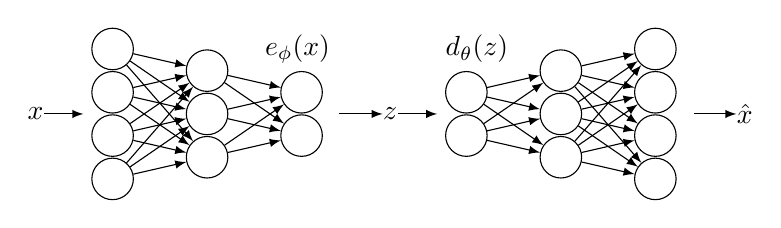
\begin{tikzpicture}
  \node[const]                               (x) {$x$};
  \node[const, right = 0.5cm of x]           (xin) {};
  % encoder in
  \node[latent, right = 0.6cm of x, yshift = 0.825cm] (E11) {};
  \node[latent, right = 0.6cm of x, yshift = 0.275cm] (E12) {};
  \node[latent, right = 0.6cm of x, yshift = -0.275cm] (E13) {};
  \node[latent, right = 0.6cm of x, yshift = -0.825cm] (E14) {};
  % encoder hidden
  \node[latent, right = 1.8cm of x, yshift = 0.55cm] (E21) {};
  \node[latent, right = 1.8cm of x, yshift = 0cm] (E22) {};
  \node[latent, right = 1.8cm of x, yshift = -0.55cm] (E23) {};
  % encoder out
  \node[latent, right = 3cm of x, yshift = 0.275cm] (E31) {};
  \node[latent, right = 3cm of x, yshift = -0.275cm] (E32) {};
  % encoder tag
  \node[const, right = 2.8cm of x, yshift = 0.825cm] (E) {$e_{\phi}(x)$};
  % code
  \node[const, right = 4.3cm of x]           (z) {$z$};
  \node[const, right = -0.8cm of z]           (zout) {};       
  \node[const, right = 0.5cm of z]           (zin) {};
  % decoder in
  \node[latent, right = 0.6cm of z, yshift = 0.275cm] (D11) {};
  \node[latent, right = 0.6cm of z, yshift = -0.275cm] (D12) {};
  % decoder hidden
  \node[latent, right = 1.8cm of z, yshift = 0.55cm] (D21) {};
  \node[latent, right = 1.8cm of z, yshift = 0cm] (D22) {};
  \node[latent, right = 1.8cm of z, yshift = -0.55cm] (D23) {};
  % decoder out
  \node[latent, right = 3cm of z, yshift = 0.825cm] (D31) {};
  \node[latent, right = 3cm of z, yshift = 0.275cm] (D32) {};
  \node[latent, right = 3cm of z, yshift = -0.275cm] (D33) {};
  \node[latent, right = 3cm of z, yshift = -0.825cm] (D34) {};
  % xhat
  \node[const, right = 4.3cm of z]           (xhat) {$\hat{x}$};
  \node[const, right = -0.8cm of xhat]       (xhatout) {};       
  % decoder tag
  \node[const, right = 0.6cm of z, yshift = 0.825cm] (D) {$d_{\theta}(z)$};
  

  % edges
  \nedge {x} {xin}
  % encoder 
  \nedge {E11, E12, E13, E14} {E21, E22, E23}
  \nedge {E21, E22, E23} {E31, E32}
  % latent
  \nedge {zout} {z}
  \nedge {z} {zin}
  % decoder
  \nedge {D11, D12} {D21, D22, D23}
  \nedge {D21, D22, D23} {D31, D32, D33, D34} 
  %xhat
  \nedge {xhatout} {xhat}

  % encoder plate
%  \plate {E} {(E11)(E14)(E32)} {};
\end{tikzpicture}

\par\end{centering}
\centering{}\caption{An example of an autoencoder consisting of fully connected layers.
The latent code $z\in\mathbb{R}^{2}$ is computed by propagating the
input $x\in\mathbb{R}^{4}$ through the encoder $e_{\phi}(x)$ and
then used to produce the reconstruction $\hat{x}\in\mathbb{R}^{4}$
via the decoder $d_{\theta}(z)$.}
\label{fig:ae}
\end{figure}

The basic idea of using an \textbf{autoencoder} (AE) for anomaly detection
is simple and was used e.g. in \cite{sakurada2014anomaly,thompson2002implicit}.
An autoencoder is a neural net that tries to propagate an input data
sample through multiple layers and produce an output that is as similar
to the input as possible. While this seems to be rather uninteresting,
the trick is that the architecture of an autoencoder is usually constrained
in such a way that the hidden layers contain less neurons than the
input and output layers, therefore preventing the autoencoder from
learning identity and forcing it to compress the data in the most
efficient way. A standard autoencoder architecture can be seen in\,\ref{fig:ae}.
It usually consists of two parts -- the decoder and encoder. Suppose
that $\mathcal{X}$ is the space of the input data and $x\in\mathcal{X}$
is an element of that space, while $\mathcal{Z}$ is the space of
samples produced by the encoder, also called the latent space. Then
we can define the encoder as a projection $e_{\phi}:\mathcal{X}\rightarrow\mathcal{Z}$
and the decoder as $d_{\theta}:\mathcal{Z}\rightarrow\mathcal{X}$.
Trainable hidden parameters (weights) of the neural network are denoted
by $\phi$ and $\theta$. Both parts of an autoencoder are trained
(the weights are adapted) using backpropagation\,\cite{werbos1982applications}
to minimize the reconstruction error with respect to $\phi$ and $\theta$

\begin{equation}
\mathcal{L}_{r}(x,\phi,\theta)=||x-d_{\theta}(e_{\phi}(x))||_{2}^{2}.\label{eq:ae_loss}
\end{equation}
The process of training and autoencoder is describe in Alg. \ref{alg:ae_train}.
Any standard optimization procedure based on gradient descent can
be used for updating in the step 6, such as the Nesterov optimizer\,\cite{nesterov1983method},
ADAM\,\cite{kingma2014adam} or AMSGrad\,\cite{reddi2019convergence}.
\begin{algorithm}

\begin{algorithmic}[1]
\Require{Autoencoder $(g_{\vc{\theta}}, e_{\vc{\phi}})$, a training set $X=\lbrace \vc{x}_1, \vc{x}_2, \ldots, \vc{x}_n \rbrace \subset \mathcal{X}$, maximum number of iterations $I\in\mathbb{N}$, batchsize $B \in \mathbb{N}$.}
\State $\vc{\phi},\vc{\theta} \gets $ Initialize weights
\State{$i \gets $ Iteration counter}
\While{$i<I$ or $\vc{\phi},\vc{\theta}$ are not converged}
	\State{$X_B \gets$ A random batch of $B$ samples from $X$}
	\State$l \gets \frac{1}{B}\sum_{i=1}^B \mathcal{L}_{\text{AE}}(\vc{x}_i,\vc{\phi},\vc{\theta}), \vc{x}_i \in X_B$
	\State$\vc{\phi} \stackrel{+}\gets - \nabla_{\vc{\phi}}l $ update of encoder weights
	\State$\vc{\theta} \stackrel{+}\gets - \nabla_{\vc{\theta}}l $ update of decoder weights
	\State{$i \gets i+1$}
\EndWhile
\State{\textbf{return} encoder $e_{\vc{\phi}}(\vc{x})$, decoder $g_{\vc{\theta}}(\vc{z})$}
\end{algorithmic}\caption{Autoencoder training procedure}
\label{alg:ae_train}

\end{algorithm}

\begin{figure}
\begin{centering}
\includegraphics[scale=0.85]{data/chapter_intro/ae_reconstruction}\caption{The figure demonstrates the ability of an autoencoder to reconstruct
data. The dimensionality of the latent space $\mathcal{Z}$ is on
the x--axis, while the average reconstruction error over the whole
dataset is on the y--axis. Note that although the artificial dataset
is 16--dimensional, it only contains 8 non--correlated dimensions
while the remaining are a linear combination of them. This results
in the error dropping to zero for $\text{dim}(\mathcal{Z})>=8$ where
the model is able to disentangle the correlations and learn the identity
function.}
\label{fig:ae_reconstruction}
\par\end{centering}
\end{figure}

Suppose that $p(x)$ is the distribution of the normal data in $\mathcal{X}$
space. After training with enough examples sampled from $p(x)$, an
autoencoder should be able to reconstruct any sample from $p(x)$
almost exactly with the average error given by the constraints of
the hidden layers, as demonstrated in \ref{fig:ae_reconstruction}.
In other words, the autoencoder has learnt the shape of the distribution.
When presented with a novel sample, the ability of the autoencoder
to reconstruct it might be used to decide whether the sample comes
from $p(x)$ or not. Indeed, the most naive way of using autoencoders
for anomaly detection is assuming that $p(x)$ is the distribution
of normal data and training them using normal samples. Then, for a
novel sample $x$ the reconstruction error of the trained network
($\bar{\phi}$ and $\bar{\theta}$ are the learnt parameters of the
autoencoder)

\begin{equation}
f_{AE}(x)=\mathcal{L}_{r}(x,\bar{\phi},\bar{\theta})\label{eq:ae_score}
\end{equation}
can be used as a an anomaly score function with the assumption that
an anomaly is going to produce a larger reconstruction error due to
not coming from $p(x)$.


\subsection{Ensemble-based}

MOGAAL

\subsection{Hybrid - two-stage models}

\subsection{self-supervised methods}

\section{Anomaly detection datasets}


\chapter{Overview of generative models in anomaly detection}

\section{The Variational Autoencoder}

The Variational Autoencoder (VAE) model is a generative model based
on the classical autoencoder (AE). In its basic form, the architecture
is indeed very similar to that of an AE. The main difference is that
unlike in AE, where the encoding to latent space $\mathcal{Z}$ is
not constrained from taking any shape or form as far as the learning
objective is minimized, in VAE a desired shape of the encoding is
explicitly prescribed in the form of a prior distribution $p(z)$.
If the network is trained properly and the encoder is not far from
the desirable shape, we can feed samples from $p(z)$ to the decoder
and expect to obtain random samples in the $\mathcal{X}$ space that
will however resemble those from the training dataset. This is the
simple explanation of how VAE works --- we will dwell into the details
in the following text.

The VAE has enjoyed a great success in a number of fields since its
introduction in\,\cite{kingma2013vae}. Its has been mainly used
for generation of artificial images such as faces\,\cite{rezende2014stochastic}
but also for other tasks such as semi--supervised learning\,\cite{kingma2014semi},
segmentation\,\cite{sohn2015learning}, static image forecasting\,\cite{walker2016uncertain}
and of course for anomaly detection\,\cite{an2015variational,xu2018unsupervised,solch2016variational}.
Since its popularity, a multitude of approaches enhancing the original
VAE has been published, approaching the paradigm from different angles,
with some of the more prominent examples published in\,\cite{higgins2017beta,zhao2017infovae,tolstikhin2017wasserstein,makhzani2015adversarial,pu2017adversarial}.
In the following text, we will go through the basic theory and its
implications for the basic VAE and then through some of the extensions.
Also, we will try to assess the suitability of the presented models
for anomaly detection.

\subsection{Probabilistic foundations}

We will begin by defining the Variational Autoencoder from a probabilistic
perspective. In fact, the connection with autoencoders will become
apparent only after all the derivations have been carried out. Let
us assume that there is a dataset $X=\{x_{i}\}_{i=1}^{N}$ consisting
of i.i.d samples. We want to obtain a tractable estimate of the true
data distribution $p(x)$ in order to be able to sample from it. For
that purpose, suppose that there is a hidden random process that generates
the data and which involves a latent variable $z$. Then, we can redirect
the sampling from the data space $\mathcal{X}$ to the latent space
$\mathcal{Z}$, in which it might be easier. Specifically, we want
to sample from the latent distribution specified by density $p(z)$,
then pass this to the generative model distribution $p_{\theta}(x|z)$
with parameters $\theta$ and obtain a sample $x$ that will be very
similar to the samples coming from $p(x)$. In other words, we want
to maximize the probability of each sample obtained through the generative
process
\begin{equation}
p_{\theta}(x)=\int_{\mathcal{Z}}p_{\theta}(x|z)p(z)dz.\label{eq:x_likelihood}
\end{equation}
Unfortunately, there are several issues with this. Firstly, we do
not know the optimal value of parameters $\theta$. Secondly, the
integral\,(\ref{eq:x_likelihood}) is usually intractable, e.g. in
the case where $p_{\theta}(x|z)$ is represented by a neural network.
Finally, we want to avoid expensive sampling methods such as Monte
Carlo Expectation Maximization which might offer a solution. We will
use a sampling procedure in the end, but we only want to pass such
samples $z$ to the generative model that will already be very likely
under $p_{\theta}(x|z)$. To this end, we introduce a recognition
model $q_{\phi}(z|x)$ which is an approximation of the true intractable
posterior $p(z|x)$ parametrized by $\phi$.

\subsection{The ELBO objective}

Now, we would like to relate all the introduced probability distributions
together in way that would enable us to optimize the recognition and
the generative model in respect to $\phi,\theta$. Continuing from\,(\ref{eq:x_likelihood}),
\begin{equation}
\ln p_{\theta}(x)=\mathbb{E}_{q_{\phi}(z|x)}\left[\ln p_{\theta}(x)\right]=\mathbb{E}_{q_{\phi}(z|x)}\left[\ln p_{\theta}(x|z)+\ln p(z)-\ln p(z|x)\right],
\end{equation}
where we have used the Bayes' rule and the fact that $p_{\theta}(x)$
does not depend on $z$. Now we recall the definition of the KL divergence\,(\ref{eq:kld})
\begin{eqnarray}
\ln p_{\theta}(x)-D_{\text{KL}}\left(q_{\phi}(z|x)||p(z|x)\right) & = & \mathbb{E}_{q_{\phi}(z|x)}\left[\ln p_{\theta}(x|z)+\ln p(z)-\ln q_{\phi}(z|x)\right]\label{eq:elbo1}\\
 & = & \mathbb{E}_{q_{\phi}(z|x)}\left[\ln p_{\theta}(x|z)\right]-D_{\text{KL}}\left(q_{\phi}(z|x)||p(z)\right)\label{eq:elbo2}\\
 & = & \mathcal{L}(x,\phi,\theta)\label{eq:elbo3}
\end{eqnarray}
Now, we have a variational lower bound $\mathcal{L}(x,\phi,\theta)$
(sometimes called ELBO -- evidence lower boundary) through which
we can optimize the marginal likelihood $p_{\theta}(x)$. This is
due to the fact that the analytically unsolvable term $D_{\text{KL}}\left(q_{\phi}(z|x)||p(z|x)\right)$
is always nonnegative, thus by maximization of $\mathcal{L}(x,\phi,\theta)$
we also maximize $p_{\theta}(x)$.

Let us dissect the individual parts of the above equation. By looking
at the individual parts of Eq.\,(\ref{eq:elbo2}), we can see that
by maximizing the ELBO, we simultaneously maximize the likelihood
$p_{\theta}(x|z)$ and minimize the distance between $q_{\phi}(z|x)$
and $p(z)$. While looking at the left--hand side of (\ref{eq:elbo1})
we can see that in the same process, the marginal likelihood $p_{\theta}(x)$
is maximized and the error term $D_{\text{KL}}\left(q_{\phi}(z|x)||p(z|x)\right)$
is minimized, forcing the shape of $q_{\phi}(z|x)$ to the true posterior.
Also, from\,(\ref{eq:elbo2}) it is now apparent why this model is
called an autoencoder. We pass $x$ to the recognition model (encoder),
produce latent $z$ and pass this back to the generative model (decoder)
to obtain a reconstructed sample.
\begin{figure}
\centering{}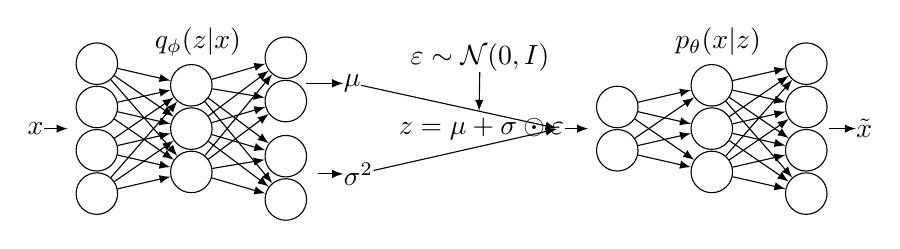
\begin{tikzpicture}
  \node[const]                               (x) {$x$};
  \node[const, right = 0.3cm of x]           (xin) {};
  % encoder in
  \node[latent, right = 0.4cm of x, yshift = 0.825cm] (E11) {};
  \node[latent, right = 0.4cm of x, yshift = 0.275cm] (E12) {};
  \node[latent, right = 0.4cm of x, yshift = -0.275cm] (E13) {};
  \node[latent, right = 0.4cm of x, yshift = -0.825cm] (E14) {};
  % encoder hidden
  \node[latent, right = 1.6cm of x, yshift = 0.55cm] (E21) {};
  \node[latent, right = 1.6cm of x, yshift = 0cm] (E22) {};
  \node[latent, right = 1.6cm of x, yshift = -0.55cm] (E23) {};
  % encoder out
  \node[latent, right = 2.8cm of x, yshift = 0.9cm] (E31) {};
  \node[latent, right = 2.8cm of x, yshift = 0.35cm] (E32) {};
  \node[latent, right = 2.8cm of x, yshift = -0.35cm] (E33) {};
  \node[latent, right = 2.8cm of x, yshift = -0.9cm] (E34) {};
  % encoder tag
  \node[const, right = 1.4cm of x, yshift = 1.1cm] (E) {$q_{\phi}(z|x)$};
  % code
  \node[const, right = 3.8cm of x, yshift = 0.575cm]           (mu) {$\mu$};
  \node[const, right = 3.8cm of x, yshift = -0.575cm]           (sigma) {$\sigma^2$};
  \node[const, right = -0.75cm of mu]           (muout) {};       
  \node[const, right = -0.75cm of sigma]           (sigmaout) {};       
  \node[const, right = 4.5cm of x]           (z) {$z=\mu+\sigma \odot \varepsilon$};
  \node[const, right = -0.1cm of z]           (zout) {};
  \node[const, right = 4.65cm of x, yshift = 0.9cm]         (epsilon) {$\varepsilon \sim \mathcal{N}(0,I)$};
  \node[const, right = 5.5cm of x, yshift = 0.2cm]         (epsilonin) {};
  \node[const, right = 0.3cm of z]           (zin) {};
  % decoder in
  \node[latent, right = 0.4cm of z, yshift = 0.275cm] (D11) {};
  \node[latent, right = 0.4cm of z, yshift = -0.275cm] (D12) {};
  % decoder hidden
  \node[latent, right = 1.6cm of z, yshift = 0.55cm] (D21) {};
  \node[latent, right = 1.6cm of z, yshift = 0cm] (D22) {};
  \node[latent, right = 1.6cm of z, yshift = -0.55cm] (D23) {};
  % decoder out
  \node[latent, right = 2.8cm of z, yshift = 0.825cm] (D31) {};
  \node[latent, right = 2.8cm of z, yshift = 0.275cm] (D32) {};
  \node[latent, right = 2.8cm of z, yshift = -0.275cm] (D33) {};
  \node[latent, right = 2.8cm of z, yshift = -0.825cm] (D34) {};
  % xhat
  \node[const, right = 3.7cm of z]           (xhat) {$\tilde{x}$};
  \node[const, right = -0.6cm of xhat]       (xhatout) {};    
  % decoder tag
  \node[const, right = 1.4cm of z, yshift = 1.1cm] (D) {$p_{\theta}(x|z)$};   
  

  % edges
  \nedge {x} {xin}
  % encoder 
  \nedge {E11, E12, E13, E14} {E21, E22, E23}
  \nedge {E21, E22, E23} {E31, E32, E33, E34}
  % latent
  \nedge {muout} {mu}
  \nedge {sigmaout} {sigma}
  \nedge {mu,sigma} {zout}
  \nedge {z} {zin}
  \nedge {epsilon} {epsilonin}
  % decoder
  \nedge {D11, D12} {D21, D22, D23}
  \nedge {D21, D22, D23} {D31, D32, D33, D34} 
  %xhat
  \nedge {xhatout} {xhat}
\end{tikzpicture}
\caption{A schematic of a Variational Autoencoder consisting of fully connected
layers with the encoder $q_{\phi}(z|x)$ parametrizing a normal distribution.
A mean $\mu$ and variance vector $\sigma^{2}$ are extracted from
the last layer of the encoder. They are used to sample a code $z$
from the corresponding normal distribution and then passed to the
decoder $p_{\theta}(x|z)$ to produce the reconstruction $\tilde{x}.$}
\label{fig:vae}
\end{figure}


\subsection{The reparametrization trick}

Often, the KL divergence in\,(\ref{eq:elbo2}) can be computed analytically
based on our choice of $p(z)$. Furthermore, to optimize the ELBO,
we need to sample from $q_{\phi}(z|x)$. A usual choice of the prior
is $p(z)=\mathcal{N}(z|0,I)$, but any continuous distribution is
theoretically viable. In tandem with this, the shape of the recognition
distribution should be the same, i.e. $q_{\phi}(z|x)=\mathcal{N}(z|\mu_{\phi}(x),\Sigma_{\phi}(x))$.
This is however problematic for training through backpropagation,
because sampling is not a differentiable operation. Therefore, to
be able to optimize $\phi$, a reparametrization trick must be used.
Instead of drawing samples $z\sim\mathcal{N}(z|\mu_{\phi}(x),\Sigma_{\phi}(x))$,
we first take a sample from noise distribution $\varepsilon\sim p(\varepsilon)=\mathcal{N}(0,1)$
and then compute $z=\mu_{\phi}(x)+\Sigma_{\phi}^{1/2}(x)\varepsilon$.
This changes the ELBO to
\begin{equation}
\mathcal{L}(x,\phi,\theta)=\mathbb{E}_{\varepsilon\sim\mathcal{N}(0,I)}\left[\ln p_{\theta}(x|z=\mu_{\phi}(x)+\Sigma_{\phi}^{1/2}(x)\varepsilon)\right]-D_{\text{KL}}\left(q_{\phi}(z|x)||p(z)\right).\label{eq:vae_loss}
\end{equation}
Note that in practice, where encoder $q_{\phi}(x|z)$ is represented
by a neural network, the distribution parameters are extracted from
its last layer. While linear activation is used for $\mu_{\phi}(x)$,
softplus is usually used for $\Sigma_{\phi}(x)$.

\subsection{Vanilla VAE\label{sec:vae_vanilla}}

In this section we will describe the single most common VAE architecture
with the recognition model being $q_{\phi}(z|x)=\mathcal{N}(z|\mu_{\phi}(x),\text{diag}(\sigma_{\phi}^{2}(x))),\mu_{\phi}(x),\sigma_{\phi}^{2}(x)\in\mathbb{R}^{d}$.
This, together with the fact that $p(z)=\mathcal{N}(z|0,I)$ makes
the computation of the KL divergence in\,(\ref{eq:elbo2}) analytically
tractable, see\,(\ref{eq:kl_standard}). The ELBO for a single datapoint
then takes the form
\begin{eqnarray*}
\mathcal{L}(x,\phi,\theta;\varepsilon) & = & \frac{1}{M}\sum_{m=1}^{M}\ln p_{\theta}(x|z^{m}(\varepsilon))+\frac{1}{2}\sum_{i=1}^{d}\left(1-\left(\sigma_{\phi}^{2}(x)\right)_{i}+\ln\left(\sigma_{\phi}^{2}(x)\right)_{i}-\left(\mu_{\phi}^{2}(x)\right)_{i}\right)
\end{eqnarray*}
\begin{equation}
\text{where }z^{m}(\epsilon)=\mu_{\phi}(x)+\sigma_{\phi}(x)\odot\varepsilon,\varepsilon\sim\mathcal{N}(0,I).\label{eq:vae_elbo1}
\end{equation}
The expectation for the marginal likelihood is replaced with a mean
over $M$ samples of $\varepsilon\sim p(\varepsilon)$ and $\odot$
denotes an element--wise product. Note that $M=1$ is usually sufficient
given that the model is trained with high enough batchsize. Now, $p_{\theta}(x|z)$
can take the form of any suitable distribution (e.g. normal or Bernoulli).
The most common choice is the case of a normal isotropic generative
model, that is $p_{\theta}(x|z)=\mathcal{N}(x|\mu_{\theta}(z),\Sigma_{\theta}(z))=\mathcal{N}(x|\mu_{\theta}(z),\sigma I),\sigma\in\mathbb{R}$.
Then, the optimization objective becomes
\begin{equation}
\mathcal{L_{\text{VAE}}}(x,\phi,\theta;\varepsilon)=-\frac{1}{\sigma M}\sum_{m=1}^{M}||x-\mu_{\theta}(z^{m}(\varepsilon))||_{2}^{2}+\frac{1}{2}\sum_{i=1}^{d}\left(1-\left(\sigma_{\phi}^{2}(x)\right)_{i}+\ln\left(\sigma_{\phi}^{2}(x)\right)_{i}-\left(\mu_{\phi}^{2}(x)\right)_{i}\right)\label{eq:vae_elbo2}
\end{equation}
with $z^{m}(\varepsilon)$ sampled in the same way as in\,(\ref{eq:vae_elbo1}).
Finally, this objective can be optimized via stochastic gradient descent\,\cite{bottou2010large}.

See Fig.\,\ref{fig:vae} for a schematic example of a VAE architecture
that uses the loss function\,(\ref{eq:vae_elbo2}). The training
procedure of a VAE is described in Alg.\,\ref{alg:vae_train}. Note
that instead of setting a fixed variance parameter $\sigma$ in the
decoder, one can optimize and extract it instead from the last layer
of the decoder, either as a scalar $\Sigma_{\theta}(z)=\sigma_{\theta}(z)I,\sigma(z)\in\mathbb{R}$
or even full diagonal of the covariance $\Sigma_{\theta}(z)=\text{diag}\left(\sigma_{\theta}(z)\right)I,\sigma(z)\in\mathbb{R}^{n}$
where $n$ is the dimensionality of input space $\mathcal{X}$. See
the discussion in Fig.\,\ref{fig:betavae} for details.

\begin{algorithm}
\begin{algorithmic}[1]
\Require{A training set $X=\lbrace x_j \rbrace \in \mathbb{R}^d$, maximum number of iterations $I\in\mathbb{N}$, batchsize $L \in \mathbb{N}$, the number of decoder samples $M$.}
\State $\phi,\theta \gets $ Initialize parameters
\State{$i \gets $ Iteration counter}
\While{$i<I$ or $\phi,\theta$ are not converged}
	\State{$X_L \gets$ A random batch of $L$ samples from $X$}
	\State{$\lbrace \varepsilon_j \rbrace_{j=1}^L \gets$ Random samples from $\mathcal{N}(0,I)$}
	\State$l \gets \frac{1}{L}\sum_{j=1}^L \mathcal{L}_\text{VAE}(x_j,\phi,\theta;\varepsilon_j), x_j \in X_L$
	\State$\phi,\theta \gets $ Update parameters with gradients $\nabla_{\theta,\phi} l$ to maximize $l$
	\State{$i \gets i+1$}
\EndWhile
\State{\textbf{return} encoder $q_{\phi}(z|x)$, decoder $p_{\theta}(x|z)$}
\end{algorithmic}\caption{Variational Autoencoder training procedure.}
\label{alg:vae_train}
\end{algorithm}

Now that a VAE model is trained, we can finally use it to generate
realistic samples. Because we have pushed the encoding distribution
to be close to the prior while maximizing the marginal probability
of the encoding to produce a reasonable reconstruction through the
decoder, we can expect the converged decoder to be able to transform
samples $z\sim\mathcal{N}(0,1)$ to the $\mathcal{X}$ space in such
a manner that they will be very close to the samples from the training
dataset. This is also a place to note why we are using neural network
representation of $q_{\phi}(z|x)$ and $p_{\theta}(x|z)$. Since NNs
have be proven to be universal function approximators, we know that
given enough capacity, data and training time, the decoder can learn
a mapping from $\mathcal{N}(0,1)$ to arbitrary function.

What is of a greater interest to us from the anomaly detection perspective
is reconstructing a sample using the trained VAE. This is done through
the same process the VAE is trained, thus by reconstruction of $x$
we understand $\hat{x}$ such that
\begin{equation}
\hat{x}\sim\mathcal{N}(x|\mu_{\theta}(z),\Sigma_{\theta}(z)),z\sim q_{\phi}(z|x).
\end{equation}
We simply pass $x$ to the encoder $q_{\phi}(z|x)$, obtain the parameters,
sample from the noise distribution and pass the resulting $z$ to
the decoder $p_{\theta}(x|z)$ to obtain the generative distribution
from which we can readily sample.

Looking at the objective\,(\ref{eq:vae_elbo2}) we can see the connection
with an ordinary autoencoder. The objective can be decomposed into
a reconstruction term and a regularization term on the latent space.
The one advantage of a VAE over AE is that provides a distribution
both in the latent and sample space that can be readily sampled from,
while the autoencoder is completely deterministic. This, coupled with
the regularization term, enables the VAE to generalize better.

It has been shown in\,\cite{doersch2016tutorial} that scaling of
the VAE loss\,(\ref{eq:vae_elbo2}) with respect to the variance
estimated by the encoder does not make much sense. It is however possible
to scale the contribution of the two losses to the total loss, as
was done in\,\cite{higgins2017beta}, such that
\begin{equation}
\mathcal{L}(x,\phi,\theta,\beta)=\mathbb{E}_{q_{\phi}(z|x)}\left[\ln p_{\theta}(x|z)\right]-\beta D_{\text{KL}}\left(q_{\phi}(z|x)||p(z)\right),\beta>0.\label{eq:betavae}
\end{equation}
Varying the value of $\beta$ puts a different emphasis on how much
should the latent space be regularized. Higher values of $\beta$
supposedly lead to better representation power, however in some of
our experiments we have used $\beta<1$ in order to pronounce the
importance of the reconstruction error. Again, the discussion under
Fig.~\ref{fig:betavae} contains some details on this.

\begin{figure}
\centering
    \begin{subfigure}[b]{0.45\textwidth}
        \centering
        \includegraphics[scale=0.9]{data/chapter_survey/vae_two_moons_z1_colored}
        \caption{$\text{dim}(\mathcal{Z})=1$}
    \end{subfigure}
    \begin{subfigure}[b]{0.45\textwidth}
        \centering
        \includegraphics[scale=0.9]{data/chapter_survey/vae_two_moons_z2_colored}
        \caption{$\text{dim}(\mathcal{Z})=2$}
    \end{subfigure}
\caption{An overview of VAE behaviour with respect to the scaling parameter
$\beta$ of the objective\,(\ref{eq:betavae}) and to the way the
covariance of the generative model $p_{\theta}(x|z)=\mathcal{N}(x|\mu_{\theta}(z),\Sigma_{\theta}(z))$
is estimated. The VAE model was trained on the two--moons data, plotted
in the plots at the very top. Variants with 1D (a) and 2D (b) latent
spaces are compared, means of the generative model $\mu_{\theta}(z)$
are plotted on the left and the latent representations on the right.
Clearly, smaller values of $\beta$ lead to better sample reconstruction.
Also, lower preference of the KL divergence objective seems to lead
to better separation in the latent space. This is understandable,
since the prior $p(z)=\mathcal{N}(0,1)$ is unimodal. The covariance
is given by a fixed scalar ($\Sigma=\sigma I,\sigma=1$), by a scalar
estimated from the data ($\Sigma=\sigma(z)I$), or the full diagonal
of the covariance matrix is estimated ($\Sigma=\text{diag}(\sigma(z))$).
The magnitude of the estimated variance in the two latter cases is
denoted by color, where brighter color corresponds to a higher value.
It is interesting that the second case ($\Sigma=\sigma(z)I$) seems
to alleviate the reconstruction difficulties with higher $\beta$,
while the estimation of the full covariance diagonal does not exhibit
such property. Also, the third case seems to ``exploit'' the estimation
of variance -- instead of pushing and optimizing the mean, it can
instead simply put higher variance in the direction in which the reconstruction
is worse and still incur only a small loss. Due to this behaviour,
the second case seems to be the most robust and stable way of estimation
of the reconstruction variance. Not surprisingly, the 2D case provides
better reconstructions since it was provided with one more dimension
to encode data to.}
\label{fig:betavae}
\end{figure}

\begin{figure}
\centering{}\includegraphics[scale=0.8]{data/chapter_survey/mnist_reconstruction_generation}\caption{Example of a VAE trained on the MNIST dataset -- ground truth examples
are in the top row, reconstructed samples (means of $p_{\theta}(x|z)$)
are in the middle row, artificially generated digits are in the bottom
row. The reconstructions are blurry, which is a typical VAE behaviour.
Also, the reconstruction is imperfect for digits which are resemble
each other, such as 9, 4 and 7 or 3 and 8. The artificial digits were
created by linearly interpolating between two coordinates in the latent
space and using this as an input to the decoder. The VAE then presents
a smooth interpolation between digits 1 and 8.}
\label{fig:mnist_reconstruction}
\end{figure}
 
\begin{figure}
\begin{centering}
\includegraphics[scale=0.8]{data/chapter_survey/mnist_latent}
\par\end{centering}
\caption{The latent space of the MNIST dataset produced by a VAE. Note the
overlapping of some digit encodings, e.g. 7 and 9.}
\label{fig:mnist_latent}
\end{figure}

We include some experiments with the MNIST hand--written digits dataset,
which can be found in almost every VAE publication, see Fig.\,\ref{fig:mnist_reconstruction}
and \ref{fig:mnist_latent}, that demonstrate the way a VAE encodes,
reconstructs and generates new samples.

\subsection{VAE in anomaly detection}

An easy way to assess the probability of a sample coming from the
data distribution would be computing 
\begin{equation}
p_{\theta}(x)=\mathbb{E}_{p(z)}\left[\ln p_{\theta}(x|z)\right]
\end{equation}
by sampling directly from the prior. Although theoretically well--justified,
it has been shown that this does not work well enough in practice\,\cite{xu2018unsupervised}.
Instead, the reconstruction probability can be used as an anomaly
score function
\begin{equation}
f_{\text{VAE}}(x)=-\frac{1}{M}\sum_{m=1}^{M}\ln p_{\theta}(x|z^{m}(\varepsilon))\approx-\mathbb{E}_{q_{\phi}(z|x)}\left[\ln p_{\theta}(x|z)\right].\label{eq:vae_score}
\end{equation}
which was done in one of the first application of VAE in anomaly detection
in\,\cite{an2015variational}. The negative sign is used because
of the convention of higher score belonging to an anomaly. Note that
for a Gaussian decoder, equation\,(\ref{eq:vae_score}) is very similar
to the reconstruction error of a standard autoencoder with the difference
that the reconstruction probability is computed from several samples
of the noise distribution. Because there is sampling in the latent
space, this anomaly score can process the variability of the input
space in an improved way. We suppose that an anomalous sample that
the VAE has not been trained with will have a lower probability of
being correctly reconstructed, thus producing a higher anomaly score.
The authors of\,\cite{an2015variational} successfully compare VAE
with AE and PCA on several anomaly datasets while claiming that the
generative property of VAE can be used for causal analysis on the
detected anomalies.

The reason for using the reconstruction probability of a VAE instead
of a reconstruction error of AE is the improved generalization that
was described in the previous section. It is discussed in\,\cite{dai2017hidden}
that a VAE model is equivalent to a non--linear robust PCA model
and is proficient at dismissing sparse outliers. The authors also
make note of the fact that VAE is very efficient in pruning of unnecessary
latent dimensions in case when the real latent structure has lower
dimension than the chosen VAE latent space. However, sometimes\,\cite{pereira2018unsupervised}
the reconstruction error of the VAE is used, which is defined as
\begin{equation}
f_{\text{VAEr}}(x)=-\frac{1}{M}\sum_{m=1}^{M}||x-\mathbb{E}\left[p_{\theta}(x|z^{m}(\varepsilon)\right]||_{2}^{2},
\end{equation}
where only the mean of the generative distribution is compared to
the original sample $x$.

Another way of using VAE and other autoencoding models for anomaly
detection is to employ their ability to produce a low--dimensional
representation of high--dimensional data that preserves the important
relations between individual datapoints. Then, an anomaly detection
model (be it a generative or a classical one) can be trained on the
data encoded in the latent space. This two stage approach is especially
useful when the problem is in the image domain and some kind of vectorization
has to be used anyway. Also it enables the combination of countless
different approaches. Usage of this technique will be demonstrated
in one of the next chapters. It is also used in\,\cite{dai2019diagnosing},
where both stages are a VAE and the second stage has the same input
and latent space dimensionality (therefore it does not compress data
at all). Although this paper does not present an application in anomaly
detection, it shows an improvement in learning of the latent space
prior. 

In\,\cite{xu2018unsupervised} the authors present a so-called DonutVAE
with an enhanced loss function to detect anomalies in times series
data. The architecture is similar to that of a vanilla VAE, but the
loss becomes
\begin{equation}
\mathcal{L}_{\text{DVAE}}(x,\phi,\theta)=\mathbb{E}_{q_{\phi}(z|x)}\left[\beta\ln p(z)-\ln q_{\phi}(z|x)+\sum_{t=i}^{T}\alpha_{t}\ln p_{\theta}(x|z)\right],\label{eq:donutvae}
\end{equation}
where $x=\{x_{t}\}_{t=1}^{T}$ is a sliding window of the last $T$
observations. Also, $\alpha_{t}=0$ if $x_{t}$ is anomalous or missing
and $\alpha_{t}=1$ otherwise and $\beta=\sum_{t=1}^{T}\alpha_{t}/T$.
The authors then show that usage of this loss function improves overall
results. This however has a caveat -- known anomalous samples must
be available, otherwise the loss\,(\ref{eq:donutvae}) is the same
as\,(\ref{eq:elbo2}). Furthermore, the authors claim that using
reconstruction probability\,(\ref{eq:vae_score}) can be seen as
a weighted kernel density estimate.

The authors of\,\cite{zong2018deep} couple an ordinary autoencoder
with a Gaussian mixture model (GMM) represented by a neural network.
The AE reduces the problem dimension to help overcome the curse of
dimensionality, while the GMM model serves as a density estimate in
the latent space. The novelty of the method is in two facts. Firstly,
instead of training parameters of both models separately, they are
learnt jointly which improves the performance of the model. Secondly,
the input of the GMM model is not only the latent representation,
but also the reconstruction error of the sample. The loss is 
\begin{eqnarray}
\mathcal{L}_{\text{DAGMM}}(x,\phi,\theta,\omega) & = & ||x-d_{\theta}(e_{\phi}(x))||_{2}^{2}+\lambda_{1}E_{\omega}(z)+\lambda_{2}P(\hat{\Sigma)}\\
z & = & \left[e_{\phi}(x),||x-d_{\theta}(z)||_{2}^{2}\right]^{T}\\
E_{\omega}(z) & = & -\ln\left(\sum_{i=1}^{d}\pi_{\omega,i}\frac{\exp\left(-\frac{1}{2}(z-\mu_{\omega,i})^{T}\Sigma_{i}^{-1}(z-\mu_{\omega,i})\right)}{\sqrt{|2\pi\Sigma_{\omega,i}|}}\right)
\end{eqnarray}
where we recognize the reconstruction error of the AE, the energy
term $E_{\omega}(z)$ of the GMM model and a penalization $P(\Sigma)$
that prevents the covariance matrices in the GMM model to become singular,
$\lambda_{1},\lambda_{2}>0$ are scaling parameters. Parameters $\left\{ \pi_{\omega,i},\mu_{\omega,i},\Sigma_{\omega,i}\right\} _{i=1}^{d}$
are the parameters of the GMM model estimated by a neural network
with weights $\omega$. The sample energy is used as anomaly score.
Although this model is not based on VAE, we can view the energy term
as being similar to the KL divergence term in the VAE loss as it also
imposes some kind of structure in the latent space.

A VAE model couple with an LSTM recurrent neural network with attention
mechanism is used in\,\cite{pereira2018unsupervised} for detecting
anomalies in time series. They operate in the semisupervised setting,
where only labeled normal samples are used for training. Although
the authors share some interesting insights, e.g. that the VAE is
able to capture the temporal structure in the data, they do not offer
a thorough comparison with other methods.

\section{GAN--based models}

A different sort of generative deep model has been successful recently
-- the Generative Adversarial Network (GAN)\,\cite{goodfellow2014gan}.
It is based on a different perspective than the VAE model. Generally,
it is believed that the GAN model produces pictures that are more
realistic (less blurry) than that produced by VAE, at the cost of
difficult and highly unstable training\,\cite{salimans2016fmgan}
-- usually many models need to be trained in order to find a good
one. 

In a GAN, there are again two parts of the model. Instead of an encoder
and a decoder, there is a generator and a discriminator. The generator
is trying to produce samples that look like they come from the true
data distribution $p(x)$, while the discriminator is trying to recognize
true samples from the samples produced by the generator. They are
trained in tandem, so each of them iteratively improves in its task.

When introduced, GAN was successfully used to generate MNIST digits,
faces and CIFAR-10 images\,\cite{goodfellow2014gan}. Then they were
used in a multitude of different areas, such as next frame prediction
in videos\,\cite{lotter2015unsupervised}, semi--supervised learning\,\cite{salimans2016fmgan},
image--to--image translation\,\cite{zhu2016generative} or semantic
manipulation of high resolution images\,\cite{wang2018high}.

\subsection{GAN theory}

\begin{figure}
\centering{}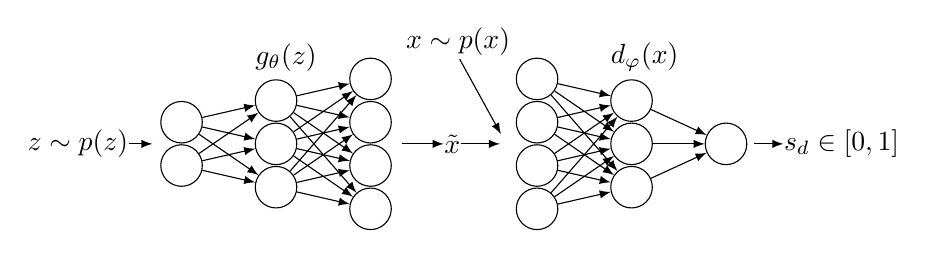
\begin{tikzpicture}
  % code
  \node[const]           (z) {$\vc{z} \sim p(\vc{z})$};
  \node[const, right = 0.3cm of z]           (zin) {};
  % decoder in
  \node[latent, right = 0.4cm of z, yshift = 0.275cm] (G11) {};
  \node[latent, right = 0.4cm of z, yshift = -0.275cm] (G12) {};
  % decoder hidden
  \node[latent, right = 1.6cm of z, yshift = 0.55cm] (G21) {};
  \node[latent, right = 1.6cm of z, yshift = 0cm] (G22) {};
  \node[latent, right = 1.6cm of z, yshift = -0.55cm] (G23) {};
  % decoder out
  \node[latent, right = 2.8cm of z, yshift = 0.825cm] (G31) {};
  \node[latent, right = 2.8cm of z, yshift = 0.275cm] (G32) {};
  \node[latent, right = 2.8cm of z, yshift = -0.275cm] (G33) {};
  \node[latent, right = 2.8cm of z, yshift = -0.825cm] (G34) {};
  % generator tag
  \node[const, right = 1.6cm of z, yshift = 1.1cm] (G) {$g_{\vc{\theta}}(\vc{z})$};
  % x
  \node[const, right = 4.0cm of z]           (xg) {$\tilde{\vc{x}}$};
  \node[const, right = -0.8cm of xg]          (xout) {};
  \node[const, right = 0.5cm of xg]           (xin) {};
  \node[const, right = -0.7cm of xg, yshift=1.3cm]      (x) {$\vc{x} \sim p(\vc{x})$};
  \node[const, right = -0.05cm of xg, yshift=1.1cm]      (xpout) {};
  \node[const, right = 0.5cm of xg, yshift=0.1cm]      (xpin) {};
  % encoder in
  \node[latent, right = 0.7cm of xg, yshift = 0.825cm] (D11) {};
  \node[latent, right = 0.7cm of xg, yshift = 0.275cm] (D12) {};
  \node[latent, right = 0.7cm of xg, yshift = -0.275cm] (D13) {};
  \node[latent, right = 0.7cm of xg, yshift = -0.825cm] (D14) {};
  % encoder hidden
  \node[latent, right = 1.9cm of xg, yshift = 0.55cm] (D21) {};
  \node[latent, right = 1.9cm of xg, yshift = 0cm] (D22) {};
  \node[latent, right = 1.9cm of xg, yshift = -0.55cm] (D23) {};
  % encoder out
  \node[latent, right = 3.1cm of xg, yshift = 0cm] (D31) {};
  % xhat
  \node[const, right = 4.1cm of xg]           (dx) {$s_d \in [0,1]$};
  \node[const, right = -1.9cm of dx]       (dxout) {};       
  % discriminator tag
  \node[const, right = 1.9cm of xg, yshift = 1.1cm] (D) {$d_{\vc{\varphi}}(\vc{x})$};
  
  % edges
  % latent
  \nedge {z} {zin}
  % generator
  \nedge {G11, G12} {G21, G22, G23}
  \nedge {G21, G22, G23} {G31, G32, G33, G34} 
  
  % x 
  \nedge {xout} {xg}
  \nedge {xg} {xin}
  \nedge {xpout} {xpin}
  % discriminator
  \nedge {D11, D12, D13, D14} {D21, D22, D23}
  \nedge {D21, D22, D23} {D31}
  %xhat
  \nedge {dxout} {dx}
\end{tikzpicture}
\caption{A schematic of a GAN consisting of fully connected layers. A latent
noise sample $z\sim p(z)$ is fed to the generator $g_{\phi}(z)$
which then produces an artificial sample $\tilde{x}$. Alternatively,
a sample $x$ is sampled from the data distribution $p(x)$. Both
are passed to the discriminator $d_{\theta}(x)$ that produces a score
$s$ -- the probability that $\tilde{x}$ or $x$ comes from the
true data distribution.}
\label{fig:gan}
\end{figure}
 

The basis on which the GAN works is relatively simple. Suppose that
we have samples coming from the true data distribution $p(x),x\in\mathcal{X}$,
which we are trying to imitate. To this end we design a generator,
which is a neural network with parameters $\phi$ and which represents
a mapping $g_{\phi}(z):\mathcal{Z}\rightarrow\mathcal{X}$. Since
the generator is deterministic and we need to cover a whole distribution,
the inputs to the generator come from a prior noise distribution $p(z),z\in\mathcal{Z}$.
Then, the task is to train the generator in such a fashion that it
learns the potentially highly non--linear mapping from $p(z)$ to
$p(x)$. This is stimulated by the adversary of the generator --
the discriminator. It can be a neural network with parameters $\theta$
which represents a mapping $d_{\theta}(x):\mathcal{X}\rightarrow\left[0,1\right]$,
i.e. the probability that a sample $x$ comes from $p(x)$ rather
than from the generator.

The discriminator is trained both with true and generated samples
to maximize the probability of assigning a correct label to them,
while the generator is minimizing the probability of the discriminator
recognizing the generated sample. This can be written down as a two
player minimax game 
\begin{equation}
\min_{\phi}\max_{\theta}\mathbb{E}_{x\sim p(x)}\left[\ln d_{\theta}(x)\right]+\mathbb{E}_{z\sim p(z)}\left[\ln\left(1-d_{\theta}(g_{\phi}(z))\right)\right].\label{eq:gan_obj}
\end{equation}
It was proven that this objective has an optimum at $-\ln4$. In practice,
(\ref{eq:gan_obj}) is not used directly. That is because the term
$\ln\left(1-d_{\theta}(g_{\phi}(z))\right)$ suffers from vanishing
gradients -- when the samples from the generator are too poor in
the beginning of the training, than this terms is almost zero and
the generator is not trained. Therefore, instead of minimizing this,
we can maximize $\ln d_{\theta}(g_{\phi}(z))$ to train the generator,
which has much stronger gradients\,\cite{goodfellow2014gan}. During
training, we sample $x$ from the data and $z$ from the noise distribution
and update the generator and discriminator parameters using loss functions
\begin{equation}
\mathcal{L}_{g}(z,\phi)=\ln d_{\theta}(g_{\phi}(z)),\label{eq:gen_loss}
\end{equation}

\begin{equation}
\mathcal{L}_{d}(x,z,\theta)=\ln d_{\theta}(x)+\ln\left(1-d_{\theta}(g_{\phi}(z))\right).\label{eq:disc_loss}
\end{equation}
The training procedure of a GAN is described in Alg.\,\ref{alg:gan_train}.
Note that during training, the generator never encounters any sample
coming from $p(x)$, as clearly visible in\,(\ref{eq:gen_loss}),
but is still able to eventually learn the shape of $p(x)$. The choice
of $p(z)$ can be rather arbitrary as far as sampling from it is possible
and the generator and discriminator have sufficient capacity. This
is unlike in VAE, where standard distribution is used due to its favourable
analytical properties. In practice however, uniform or normal distribution
is usually used.

\begin{algorithm}
\begin{algorithmic}[1]
\Require{Generator $g_{\vc{\theta}}$, discriminator $e_{\vc{\phi}}$, a training set $X=\lbrace \vc{x}_1, \vc{x}_2, \ldots, \vc{x}_n \rbrace \subset \mathcal{X}$, maximum number of iterations $I\in\mathbb{N}$, batchsize $L \in \mathbb{N}$.}
\State $\vc{\theta}, \vc{\varphi} \gets $ Initialize weights
\State{$i \gets $ Iteration counter}
\While{$i<I$ or $\vc{\theta}, \vc{\varphi}$ are not converged}
	\State{$X_L \gets$ A random batch of $L$ samples from $X$}
	\State{$Z_L \gets$ A random batch of $L$ samples from $p(\vc{z})$}
	\State$l_d \gets \frac{1}{L}\sum_{j=1}^L \mathcal{L}_d(\vc{x}_j,\vc{z}_j,\vc{\varphi}), \vc{x}_j \in X_L, \vc{z}_j \in Z_L$
	\State$\vc{\varphi} \stackrel{+}\gets - \nabla_{\vc{\varphi}} l_d$ update of discriminator weights 
	\State$l_g \gets \frac{1}{L}\sum_{j=1}^L \mathcal{L}_g (\vc{z}_j,\vc{\theta}), \vc{z}_j \in Z_L$
	\State$\vc{\theta} \stackrel{+}\gets - \nabla_{\vc{\theta}} l_g$ update of generator weights
	\State{$i \gets i+1$}
\EndWhile
\State{\textbf{return} generator $g_{\vc{\theta}}(\vc{z})$, discriminator $d_{\vc{\varphi}}(\vc{x})$}
\end{algorithmic}

\caption{GAN training procedure.}
\label{alg:gan_train}

\end{algorithm}

After a GAN is successfully trained, one can use it to generate samples
that look like they come from $p(x)$ by simply passing $z\sim p(z)$
through the generator. 

\subsection{Feature matching GAN}

GAN model is famous for the instability of its training. A phenomenon
called mode collapse has been described\,\cite{goodfellow2016nips},
which happens when $p(x)$ is multimodal, but the generator distribution
collapses to a single mode. A generator that has collapsed to a single
mode of a MNIST dataset will produce only a single digit, e.g. 1,
no matter where the code is sampled from. To mitigate this issue,
several practices have been proposed\,\cite{salimans2016fmgan}.
One of them is the use of an enhanced generator cost function
\begin{equation}
\mathcal{L}_{f}(z,x,\phi)=\alpha\mathcal{L}_{g}(z,\phi)+||h_{\theta}(x)-h_{\theta}(g_{\phi}(z))||_{2}^{2},\label{eq:fmgan}
\end{equation}
where $h_{\theta}(x)$ is the output of some intermediate (e.g. the
penultimate) layer of the discriminator and $\alpha\in\mathbb{R}$
is a scaling parameter. This loss is supposed to provide improved
gradients for the generator to stabilize the training. In the following
text, a GAN model with the loss\,(\ref{eq:fmgan}) will be referred
to as feature--matching GAN (fmGAN).

\subsection{GAN in anomaly detection}

The idea of using a GAN for anomaly detection comes from the fact
that was described in the previous text, and that is the ability of
the generator to learn the true data distribution $p(x)$ and especially
the ability of the discriminator to recognize samples coming from
$p(x)$. Naturally, if trained properly, the discriminator can be
used to test whether a new sample $x$ is from the training data distribution
which is exactly the scenario in semi-- and unsupervised anomaly
detection. However using only the discriminator score might not always
be optimal, as there might be artificial modes in the $\mathcal{X}$
space to which the discriminator assigns a high score despite there
not being any training data. Therefore, a sample produced by the generator
is compared with $x$ as well.

Using a trained generator $g_{\phi}(z)$ and discriminator $d_{\theta}(x)$,
we can define the GAN anomaly score function as a weighted average
between the discriminator score and the distance between the tested
sample and a generated sample
\begin{equation}
f_{\text{GAN}}(x)=-(1-\lambda)\ln(d_{\theta}(x))+\lambda||x-g_{\phi}(z)||_{2}^{2},\label{eq:gan_score}
\end{equation}
where $\lambda\in\left[0,1\right]$ is a scaling parameter and $z\sim p(z)$
is a sample from the prior.

The paper\,\cite{schlegl2017unsupervised} introduced the use of
convolutional fmGAN model for anomaly detection in medical images.
The model is trained on healthy patients' data and then successfully
used to identify anomalies in retinal scans. The fmGAN model was also
used in\,\cite{kliger2018novelty}, where the authors test the framework
on benchmark datasets such as MNIST and CIFAR-10. GAN was also used
in\,\cite{wang2018generative} to detect anomalies in time series
data coming from industrial processes. The authors of\,\cite{perera2019ocgan}
claim to have achieved state--of--the--art results in one-class
classification through severely restricting the latent space of the
GAN combined with an autoencoder and employing an adversarial data
augmentation strategy.

As was presented, there exists some research on GANs in anomaly detection,
however it is much sparser compared to the number of papers that use
some modification of VAE. This is probably due to the poor stability
of their training. As will be shown in chapter\,\ref{chap:kdd18},
we have observed inferiority of GANs to VAE in our experiments, although
we have not tested and compared all available methods.

\section{Wasserstein Autoencoders}

A new approach to generative modeling has been published recently
in\,\cite{mescheder2017adversarial} and improved in\,\cite{tolstikhin2017wasserstein}.
The authors provide a theoretical connection between VAE and GAN models
from the perspective of optimal transport theory. Optimal transport
cost provides a way of measuring distance between distributions but
does not reportedly suffer from vanishing gradients as much as the
GAN loss. Also, the optimal transport formulation solves one of the
issues connected with VAE, which is the fact that the regularizing
KL divergence term in the VAE loss forces all the input data samples
to zero (the mean of the standard latent prior), while in Wasserstein
autoencoders (WAE) the encoding is loosened, which reportedly leads
to improved reconstruction\,\cite{tolstikhin2017wasserstein}. In
a theoretical introduction, the authors present a general autoencoder
cost function based on the Wasserstein distance between the latent
prior and the encoder posterior distribution. Afterwards, two models
are derived by selecting a specific form of the distance. Here we
will do the same.

 

A general Wasserstein autoencoder consists of a decoder distribution
$p_{\theta}(x|z)$, encoder distribution $q_{\phi}(z|x)$ and a latent
prior $p(z)$. The decoder and encoder are both represented by neural
networks with parameters $\phi,\theta$. Also, we specify the marginal
distribution $q_{\phi}(z)=\mathbb{E}_{x\sim p(x)}\left[q_{\phi}(z|x)\right]$,
that is the distribution of the encoding in the latent space. Next,
we use the Wasserstein distance between $q_{\phi}(z)$ and $p(z)$
to regularize the training. Finally, $p_{\theta}(x)$ is the generative
model distribution that we approximate by the whole model. A general
form of the WAE loss to be minimized was derived in\,\cite{tolstikhin2017wasserstein}
and has the form
\begin{equation}
D_{\text{WAE}}(p(x),p_{\theta}(x))=\inf_{q_{\phi}(z|x)}\mathbb{E}_{x\sim p(x)}\mathbb{E}_{z\sim q_{\phi}(z|x)}\left[c(x,p_{\theta}(x|z))\right]+\lambda D_{Z}(p(z),q_{\phi}(z)),\label{eq:WAE_loss}
\end{equation}
where $c(x,p_{\theta}(x|z))$ is the reconstruction penalty term,
$D_{Z}(p(z),q_{\phi}(z))$ is a divergence measure between $q_{\phi}(z)$
and $p(z)$, and $\lambda>0$ is a scaling parameter. 

Depending on the choice of the divergence measure $D_{Z}$, different
losses and behaviours are derived for numerical optimization. Note
that\,(\ref{eq:WAE_loss}) is composed of a reconstruction error
term and a regularization term that shapes the latent space, much
like in VAE. In VAE however, the KL divergence is used to regularize
$p(z)$ and $q_{\phi}(z|x)$ which does not guarantee that the marginal
$q_{\phi}(z)$ will resemble $p(z)$. 

The commonly used reconstruction penalty term is e.g. $c(x,p_{\theta}(x|z))=||x-d_{\theta}(z)||_{2}^{2}$
in case of a deterministic decoder $d_{\theta}(x)$ or the loglikelihood
used in\,(\ref{eq:vae_elbo1}) in case of a stochastic decoder. Generation
of new samples through a Wasserstein autoencoder is simple -- one
samples $z$ from $p(z)$ and then passes this to the decoder.

\subsection{InfoVAE}

One case proposed in\,\cite{tolstikhin2017wasserstein} was for the
$D_{z}$ divergence to be the maximum mean discrepancy (MMD). This
leads to a model that was also published in\,\cite{zhao2017infovae}
under the name InfoVAE. For two probability distributions $p(z),q(z)$
the MMD is defined as
\begin{equation}
\text{MMD}_{k}(p(z),q(z))=||\int_{\mathcal{Z}}k(z,.)dp(z)-\int_{\mathcal{Z}}k(z,.)dq(z)||_{\mathcal{H}_{k}},
\end{equation}
for a positive--definite reproducing kernel $k:\mathcal{Z}\times\mathcal{Z}\rightarrow\mathbb{R}$
and $\mathcal{H}_{k}$ being a reproducing kernel Hilbert space of
real valued function mappings from $\mathcal{Z}$ to $\mathbb{R}$.
The one advantage of MMD over the KL divergence is that while KLD
only matches the first and the second moment of the two distributions,
MMD can potentially match an infinite amount of moments with the right
kernel. Some authors argue that by minimizing KLD, the latent representation
might become uninformative for the decoder to reconstruct the code.
On the other hand, MMD maximizes the mutual information between $x$
and $z$\,\cite{zhao2017infovae}. It was also reported that MMD
performs well when matching high dimensional distributions. 

If $k$ is characteristic, then MMD defines a metric and can be written
down as 
\begin{equation}
\text{MMD}_{k}(\boldsymbol{z},\boldsymbol{y})=\frac{1}{n(n-1)}\sum_{i\neq j}k(z_{i,}z_{j})+\frac{1}{n(n-1)}\sum_{i\neq j}k(y_{i,}y_{j})-\frac{2}{n^{2}}\sum_{i,j}k(z_{i,}y_{j})\label{eq:mmd}
\end{equation}
where $\boldsymbol{z}=\{z_{i}\}_{i=1}^{n},z_{i}\sim p(z),\boldsymbol{y}=\{y_{i}\}_{i=1}^{n},y_{i}\sim q(z)$
are two sets of samples sampled from the two distributions under scrutiny.
\begin{algorithm}
\begin{algorithmic}[1]
\Require{A WAE model with encoder $q_{\vc{\phi}}(\vc{z}|\vc{x})$, decoder $p_{\vc{\theta}}(\vc{x}|\vc{z})$ and a prior $p(\vc{z})$, training set $X=\lbrace \vc{x}_1, \vc{x}_2, \ldots, \vc{x}_n \rbrace \subset \mathcal{X}$, maximum number of iterations $I\in\mathbb{N}$, batchsize $B \in \mathbb{N}$, regularization coefficient $\lambda > 0$, characteristic positive definite kernel $k_f$, standard deviation parameter $\sigma$ > 0.}
\State $\vc{\phi},\vc{\theta} \gets $ Initialize parameters
\State{$i \gets $ Iteration counter}
\While{$i<I$ or $\vc{\phi},\vc{\theta}$ are not converged}
	\State{$X_B \gets$ A random batch of $B$ samples from $X$}
	\State{$Z \gets \lbrace \vc{z}_j \sim q_{\phi}(\vc{z}|\vc{x}_j), \vc{x}_j \in X_B \rbrace$ samples from the encoder}
	\State{$\tilde{Z} \gets$ A random batch of $B$ samples from prior $p(\vc{z})$}
	\State$l \gets \frac{1}{B}\sum_{j=1}^B  ||\vc{x}_j-\vc{\mu}_{\vc{\theta}}(\vc{z}_j)||_{2}^{2} +\lambda \text{MMD}_k(Z,\tilde{Z}), \vc{x}_j \in X_B, \vc{z}_j \in Z$
	\State$\vc{\phi} \stackrel{+}\gets - \nabla_{\vc{\phi}}l $ update of encoder weights
	\State$\vc{\theta} \stackrel{+}\gets - \nabla_{\vc{\theta}}l $ update of decoder weights
	\State{$i \gets i+1$}
\EndWhile
\State{\textbf{return} encoder $q_{\vc{\phi}}(\vc{z}|\vc{x})$, decoder $p_{\vc{\theta}}(\vc{x}|\vc{z})$}
\end{algorithmic}

\caption{InfoVAE training procedure.}
\label{alg:infovae}
\end{algorithm}

The two most common choices of $k(x,y)$ are the RBF and inverse multiquadratics
(IMQ) kernels. The training algorithm for a Wasserstein autoencoder
with the MMD loss is in Alg.\,\ref{alg:infovae}. Note that although
the parameters $\phi$ do not appear directly in the loss on line
7 of the algorithm, they are present through the samples $\tilde{Z_{L}}$.
Furthermore, a practical advantage of the InfoVAE over VAE is readily
apparent -- we can use a wider range of latent priors $p(z)$ since
the only restriction is that one must be able to sample from it. In
VAE however, we are forced to use a unit Gaussian prior in order to
be able to analytically compute the KL divergence term in the loss
function\,(\ref{eq:vae_loss}). 

We do not include a schematic architecture of a InfoVAE model, since
it does not differ from the VAE architecture. The forward feed of
a InfoVAE is also identical to a VAE -- the main difference is in
training.

\subsection{Adversarial Autoencoder}

A different architecture arises when the Jensen--Shannon divergence
$D_{\text{JS}}$ is used in place of $D_{Z}$. The JS divergence is
a symmetrical (unlike KL divergence) measure of distance between two
probability distributions. The use of $D_{\text{JS}}$ leads to a
model that is called adversarial autoencoder (AAE) and was originally
proposed in\,\cite{makhzani2015adversarial}. It was shown in\,\cite{tolstikhin2017wasserstein}
how the use of $D_{\text{JS}}$ leads to the use of GAN loss that
was described in the previous part. To regularize the encoder, we
add a discriminator $d_{\eta}(z):\mathcal{Z}\rightarrow\left[0,1\right]$
represented by a neural network with parameters $\eta$. The discriminator
has the same function as the one in the GAN model -- it tries to
recognize latent space samples produced by the encoder and those sampled
from the prior $p(z)$. The difference is that the discriminator now
operates on the latent space $\mathcal{Z}$ instead of the data space
$\mathcal{X}$. 

\begin{figure}
\centering{}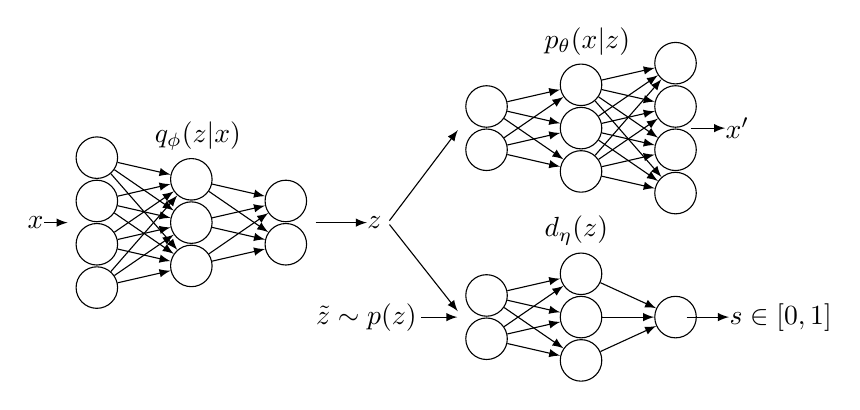
\begin{tikzpicture}
  \node[const]                               (x) {$\vc{x}$};
  \node[const, right = 0.3cm of x]           (xin) {};
  % encoder in
  \node[latent, right = 0.4cm of x, yshift = 0.825cm] (E11) {};
  \node[latent, right = 0.4cm of x, yshift = 0.275cm] (E12) {};
  \node[latent, right = 0.4cm of x, yshift = -0.275cm] (E13) {};
  \node[latent, right = 0.4cm of x, yshift = -0.825cm] (E14) {};
  % encoder hidden
  \node[latent, right = 1.6cm of x, yshift = 0.55cm] (E21) {};
  \node[latent, right = 1.6cm of x, yshift = 0cm] (E22) {};
  \node[latent, right = 1.6cm of x, yshift = -0.55cm] (E23) {};
  % encoder out
  \node[latent, right = 2.8cm of x, yshift = 0.275cm] (E31) {};
  \node[latent, right = 2.8cm of x, yshift = -0.275cm] (E32) {};
  % encoder tag
  \node[const, right = 1.4cm of x, yshift = 1.1cm] (E) {$q_{\vc{\phi}}(\vc{z}|\vc{x})$};
  % placement
  \node[const, right = 5.2cm of x, yshift=1.2cm]           (encoderin) {}; 
  \node[const, right = 5.2cm of x, yshift=-1.2cm]           (discriminatorin) {}; 
  % code
  \node[const, right = 4.1cm of x, yshift = 0cm]           (zg) {$\vc{z}$};
  \node[const, right = 3.4cm of x]           (zgout) {}; 
  \node[const, right = 0cm of encoderin]           (zgin) {};
  \node[const, right = 0.05cm of zg]           (zgout2) {};
  \node[const, right = 0cm of discriminatorin,yshift=0.05cm]           (zgin2) {};
  % prior
  \node[const, right = -1.8cm of discriminatorin, yshift = 0cm]         (z) {$\tilde{\vc{z}} \sim p(\vc{z})$};
  \node[const, right = 0cm of z, yshift = 0cm]         (zout) {};
  \node[const, right = 0cm of discriminatorin]           (zin) {};

  % decoder in
  \node[latent, right = 0.1cm of encoderin, yshift = 0.275cm] (D11) {};
  \node[latent, right = 0.1cm of encoderin, yshift = -0.275cm] (D12) {};
  % decoder hidden
  \node[latent, right = 1.3cm of encoderin, yshift = 0.55cm] (D21) {};
  \node[latent, right = 1.3cm of encoderin, yshift = 0cm] (D22) {};
  \node[latent, right = 1.3cm of encoderin, yshift = -0.55cm] (D23) {};
  % decoder out
  \node[latent, right = 2.5cm of encoderin, yshift = 0.825cm] (D31) {};
  \node[latent, right = 2.5cm of encoderin, yshift = 0.275cm] (D32) {};
  \node[latent, right = 2.5cm of encoderin, yshift = -0.275cm] (D33) {};
  \node[latent, right = 2.5cm of encoderin, yshift = -0.825cm] (D34) {};
  % xhat
  \node[const, right = 3.4cm of encoderin]           (xhat) {$\vc{x}'$};
  \node[const, right = -0.8cm of xhat]       (xhatout) {};    
  % decoder tag
  \node[const, right = 1.1cm of encoderin, yshift = 1.1cm] (D) {$p_{\vc{\theta}}(\vc{x}|\vc{z})$};   
  
  % discriminator
  \node[latent, right = 0.1cm of discriminatorin, yshift = 0.275cm] (DI11) {};
  \node[latent, right = 0.1cm of discriminatorin, yshift = -0.275cm] (DI12) {};
  % discriminator hidden
  \node[latent, right = 1.3cm of discriminatorin, yshift = 0.55cm] (DI21) {};
  \node[latent, right = 1.3cm of discriminatorin, yshift = 0cm] (DI22) {};
  \node[latent, right = 1.3cm of discriminatorin, yshift = -0.55cm] (DI23) {};
  % discriminator out
  \node[latent, right = 2.5cm of discriminatorin, yshift = 0cm] (DI31) {};
  % xhat
  \node[const, right = 3.45cm of discriminatorin]           (dx) {$s \in [0,1]$};
  \node[const, right = -1.9cm of dx]       (dxout) {};       
  % discriminator tag
  \node[const, right = 1.1cm of discriminatorin, yshift = 1.1cm] (D) {$d_{\vc{\eta}}(\vc{z})$};

  % edges
  \nedge {x} {xin}
  % encoder 
  \nedge {E11, E12, E13, E14} {E21, E22, E23}
  \nedge {E21, E22, E23} {E31, E32}
  % latent
  \nedge {zgout} {zg}
  \nedge {zgout2} {zgin}
  \nedge {zgout2} {zgin2}
  \nedge {zout} {zin}

  % decoder
  \nedge {D11, D12} {D21, D22, D23}
  \nedge {D21, D22, D23} {D31, D32, D33, D34} 
  % discriminator
  \nedge {DI11, DI12} {DI21, DI22, DI23}
  \nedge {DI21, DI22, DI23} {DI31}
  %xhat
  \nedge {xhatout} {xhat}
  %xhat
  \nedge {dxout} {dx}

\end{tikzpicture}
\caption{A schematic of a AAE model consisting of fully connected layers. A
data sample $x$ is mapped to latent space representation $\tilde{z}$
via the encoder $q_{\phi}(z|x)$. Also, a sample $z$ is sampled from
the latent prior $p(z)$. Both $z$ and $\tilde{z}$ are passed to
the discriminator $d_{\eta}(z)$ that produces a score $s$ -- the
probability that the input sample comes from the latent prior. At
the same time, the latent representation is passed to the decoder
$p_{\theta}(x|z)$ which maps it to a reconstruction $\tilde{x}$.}
\label{fig:aae}
\end{figure}

The GAN loss function\,(\ref{eq:disc_loss}) is used to train the
discriminator, while the loss function\,(\ref{eq:gen_loss}) is added
to the reconstruction term for training of the encoder and decoder.
The AAE training losses to be maximized are then
\begin{equation}
\mathcal{L}_{d}(z,\tilde{z},\eta)=\ln d_{\eta}(z)+\ln(1-d_{\eta}(\tilde{z})),\label{eq:aae_loss_disc}
\end{equation}
\begin{equation}
\mathcal{L}_{ae}(x,\tilde{x},\tilde{z},\theta,\phi)=c(x,\tilde{x})-\lambda\ln d_{\eta}(\tilde{z}),\label{eq:aae_loss_autoencoder}
\end{equation}
where $\lambda>0$, $z\sim p(z)$, $x\sim p(x)$, $\tilde{z}\sim q_{\phi}(z|x)$
and $\tilde{x}\sim p_{\theta}(x|\tilde{z})$.

\begin{algorithm}
\begin{algorithmic}[1]
\Require{A training set $X=\lbrace x_j \rbrace \in \mathbb{R}^d$, maximum number of iterations $I\in\mathbb{N}$, batchsize $L \in \mathbb{N}$, the number of decoder samples $M$, regularization coefficient $\lambda \in \mathbb{R}$.}
\State $\phi,\theta, \eta \gets $ Initialize parameters
\State{$i \gets $ Iteration counter}
\While{$i<I$ or $\phi,\theta,\eta$ are not converged}
	\State{$X_L \gets$ A random batch of $L$ samples from $X$}
	\State{$Z_L \gets$ A random batch of $L$ samples from $p(z)$}
	\State{$\tilde{Z}_L \gets \lbrace\tilde{z}_j \sim q_{\phi}(z|x_j), x_j \in X_L \rbrace$ samples from $q_{\phi}(z|x)$}
	\State{$\tilde{X}_L \gets \lbrace\tilde{x}_j \sim p_{\theta}(x|\tilde{z}_j), \tilde{z}_j \in \tilde{Z}_L \rbrace$ samples from $p_{\theta}(x|z)$}
	\State{$l_d \gets \frac{1}{L}\sum_{j=1}^L \mathcal{L}_d(z_j,\tilde{z}_j,\eta), z_j \in Z_L, \tilde{z}_j \in \tilde{Z}_L$}
	\State$\eta \gets $ Update parameters with gradients $\nabla_{\eta} l_d$ to maximize $l_d$
	\State$l_{ae} \gets \frac{1}{L}\sum_{j=1}^L \mathcal{L}_{ae}(x_j,\tilde{x}_j,\tilde{z}_j,\theta,\phi), x_j \in X_L, \tilde{x}_j \in \tilde{X}_L, \tilde{z}_j \in \tilde{Z}_L$
	\State{$\phi,\theta \gets $ Update parameters with gradients $\nabla_{\theta,\phi} l_{ae}$ to minimize $l_{ae}$}
	\State{$i \gets i+1$}
\EndWhile
\State{\textbf{return} encoder $q_{\phi}(z|x)$, decoder $p_{\theta}(x|z)$, discriminator $d_\eta(z)$}
\end{algorithmic}

\caption{AAE training procedure.}
\label{alg:aae}
\end{algorithm}

The AAE training procedure is described in Alg.\,\ref{alg:aae}.
Again, any prior $p(z)$ that we can sample from is suitable for the
regularization of AAE, even a multimodal one. A schematic of the AAE
model is in Fig.\,\ref{fig:aae}. In practice, an AAE model compared
to InfoVAE behaves similarly as GAN compared to VAE. The adversarial
loss leads to less blurry reconstructions and generated samples at
the cost of higher training instability\,\cite{tolstikhin2017wasserstein}.
One way to gain advantages of both is to use an AAE model as depicted
in Fig.\,\ref{fig:aae} and add the MMD regularization term\,(\ref{eq:mmd})
to the loss\,(\ref{eq:aae_loss_autoencoder}).


\subsection{Wasserstein autoencoders in anomaly detection}

For InfoVAE, the anomaly score can be either the reconstruction error\,(\ref{eq:ae_score})
or the reconstruction probability\,(\ref{eq:vae_score}) depending
on whether a deterministic or a stochastic decoder is used. In the
AAE model, we can use the loss of a trained model which combines the
reconstruction error term with the discriminator score 
\begin{equation}
f_{\text{AAE}}(x)=\mathcal{L}_{ae}(x,\tilde{x},\tilde{z},\bar{\theta},\bar{\phi}),\tilde{z}\sim q_{\bar{\phi}}(z|x),\tilde{x}\sim p_{\bar{\theta}}(x|\tilde{z}),\label{eq:aae_score}
\end{equation}
where $\bar{\theta},\bar{\phi}$ are fixed parameters of the trained
neural network. This anomaly score has one tuning hyperparameter $\lambda$
which governs how much the information from the discriminator weighs
in to the decision. As said before, the reconstruction term $c(x,\tilde{x})$
is either a reconstruction error or probability based on the type
of decoder.

The AAE model is used in\,\cite{leveau2017adversarial} where it
is benchmarked on the MNIST problem. Standard distribution is compared
to a Gaussian mixture model (GMM) when used as priors $p(z)$ and
a special rejection component is introduced for representation of
anomalies. 

In\,\cite{chen2018unsupervised} an AAE model is compared to the
VAE model on the task of detection of brain abnormalities in MRI images.
The loss function of the autoencoding part is enhanced by a term $\alpha||z-z^{\prime}||$,
where $z$ is a the latent representation of a sample $x$ and $z'$
is the latent representation of the reconstructed sample $\tilde{x}$.
This is supposed to improve consistency of the representation. The
thesis\,\cite{dimokranitou2017adversarial} also uses AAEs for detection
of abnormalities in videos. The model presented in\,\cite{pidhorskyi2018generative}
uses an additional discriminator on top of the decoder in AAE to improve
reconstruction and generative property. The model is then tested for
anomaly detection on standard benchmark datasets.

Clearly, some work has already been done in the area of AAE and anomaly
detection, but not a lot of authors use the InfoVAE model for this
specific task.


TODO:

\begin{itemize}
    \item read through the generativead paper and see if we are missing any models here
    \item also compare the scores etc.
\end{itemize}

\chapter{Empirical comparison of anomaly detectors}
Deep generative models are challenging the classical methods in the field of anomaly detection nowadays. Every newly published method provides evidence of outperforming its predecessors, sometimes with contradictory results. The objective of this paper is twofold: to compare anomaly detection methods of various paradigms with a focus on deep generative models and identification of sources of variability that can yield different results. The methods were compared on popular tabular and image datasets. We identified that the main sources of variability are the experimental conditions: i) the type of dataset (tabular or image) and the nature of anomalies (statistical or semantic), and ii) strategy of selection of hyperparameters, especially the number of available anomalies in the validation set. Methods perform differently in different contexts, i.e. under a different combination of experimental conditions together with computational time. This explains the variability of the previous results and highlights the importance of careful specification of the context in the publication of a new method. All our code and results are available for download.

\section{Introduction}
Deep generative models are gaining popularity in anomaly detection since the introduction of the Variational Autoencoder (VAE)~\cite{kingma2013auto}. The number of modifications and extensions of VAE or generative adversarial networks (GAN)~\cite{goodfellow2014generative} is sharply increasing, each claiming superiority over the prior art. This raises a suspicion that some of the methods are overspecialized or poorly tested. This paper, inspired by the paper "Do we need hundreds of classifiers to solve real-world classification problems?"~\cite{fernandez2014we}, strives to compare anomaly detectors under fair conditions to observe how the field has evolved in the last twenty years (the oldest compared detector~\cite{ramaswamy2000efficient} was published in 2000). Specifically, it investigates if methods based on \textit{deep} generative models offer a benefit over methods based on alternative paradigms, either the \textit{classical} methods based on distances or deep architectures without the capability of generating samples.

Indeed, there already exist comparisons of anomaly detectors. Earlier surveys~\cite{pimentel2014review, campos2016evaluation, goldstein2016comparative, pevny2016loda} do not compare to deep generative methods because they were not developed or sufficiently popular at that time. Contrary to that, the study in~\cite{kiran2018overview} contains a detailed description of deep models but provides experiments only with the basic VAE and only on specialized video datasets. Ref.~\cite{chalapathy2019deep} introduces a taxonomy of deep anomaly detection models but does not compare them experimentally. Other recent surveys~\cite{moustafa2019holistic, kwon2019survey, fernandes2019comprehensive, wang2019progress, pang2020deep} either ignore deep generative models altogether or describe them only theoretically, without making any experimental comparison. The most relevant prior art is~\cite{ruff2020unifying}, which tries to theoretically link deep and shallow techniques\footnote{The \textit{shallow} techniques corresponds to those we call \textit{classical}. We prefer the later terminology, as models based on random forests are in their essence deep, although they cannot capture semantic structure --- a touted feature of deep models}. But again, an extensive experimental comparison of different generative models is missing. One would also expect papers introducing new methods to contain such a comparison. Some of them do~\cite{pevny2016loda}, but generally, we have found comparisons limited (e.g. using a small number of datasets or methods) or flawed, which is elaborated below.

How does this paper avoid the aforementioned deficiencies? First, eight classical methods in comparison serve as a baseline, over which we expect the state-of-the-art deep methods should improve upon (latest compared method~\cite{wang2020advae} was published in 2020). Second, the comparison uses a large number of tabular (40) and image (6) datasets popular in the evaluation of deep models. Third, all methods have been given the same conditions, which primarily means the budget for optimization of hyperparameters, as~\cite{vskvara2018generative} has shown this to have a significant impact.

The list of contributions contains:
\begin{enumerate}
    \item Experimental comparison of classical and deep anomaly detectors on a large number of datasets.
    \item Identification of the dataset type, the hyperparameter selection strategy, and the computational cost as major factors in the selection of the most suitable method.
    \item We publish codes of the evaluation pipeline and compared methods, including automatic download of datasets, splitting them into training, validation, and testing, and calculating the performance metrics.
\end{enumerate}

The paper is organized as follows. In Section~\ref{sec:contexts}, the anomaly detection contexts that had the greatest influence on the outcome of our experiments are defined. In Sec.~\ref{sec:comparedmethods}, there is a brief theoretical overview of the tested generative deep models and other methods. Sec.~\ref{sec:experimentalsetup} details the datasets,  different approaches to the selection of hyperparameters, and other design decisions in the experimental setup. Sec.~\ref{sec:results} discusses the experimental results and lessons we have learned. We summarize the paper with a recommendation to practitioners and our suggestions for future work.

\section{Anomaly Detection Contexts}
\label{sec:contexts}
\begin{figure}
    \centering
    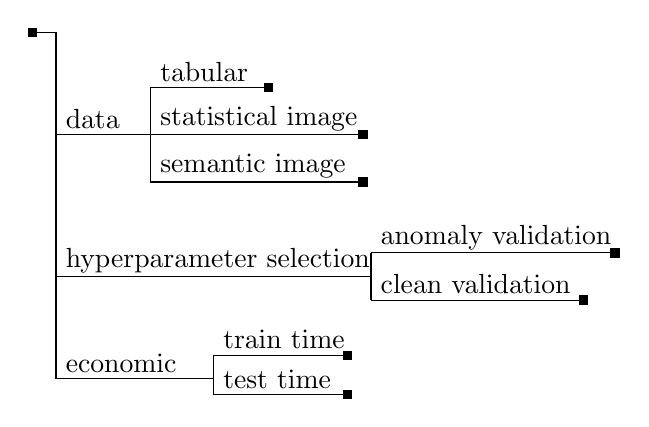
\begin{tikzpicture}
          \draw (-0.3,1.3) -- (0,1.3);
          \draw (0,1.3) -- (0,-3.1);
          
          \filldraw ([xshift=-1.5pt,yshift=-1.5pt]-0.3,1.3) rectangle ++(3pt,3pt);

          \draw (0,0) -- (1.2,0);
          \node[anchor=west] at (0,0.2) {data};
          \draw (1.2,-0.6) -- (1.2,0.6);
          \node[anchor=west] at (1.2,0.8) {tabular};
          \filldraw ([xshift=-1.5pt,yshift=-1.5pt]2.7,0.6) rectangle ++(3pt,3pt);
          \draw (1.2,0.6) -- (2.7,0.6);
          \node[anchor=west] at (1.2,0.2) {statistical image};
          \filldraw ([xshift=-1.5pt,yshift=-1.5pt]3.9,0) rectangle ++(3pt,3pt);
          \draw (1.2,0) -- (3.9,0);
          \node[anchor=west] at (1.2,-0.4) {semantic image};
          \filldraw ([xshift=-1.5pt,yshift=-1.5pt]3.9,-0.6) rectangle ++(3pt,3pt);
          \draw (1.2,-0.6) -- (3.9,-0.6);
          
          \draw (0,-1.8) -- (4,-1.8);
          \node[anchor=west] at (0,-1.6) {hyperparameter selection};
          \draw (4,-1.5) -- (4,-2.1);
          \filldraw ([xshift=-1.5pt,yshift=-1.5pt]7.1,-1.5) rectangle ++(3pt,3pt);
          \draw (4,-1.5) -- (7.1,-1.5);
          \node[anchor=west] at (4.0,-1.3) {anomaly validation};
          \filldraw ([xshift=-1.5pt,yshift=-1.5pt]6.7,-2.1) rectangle ++(3pt,3pt);
          \draw (4,-2.1) -- (6.7,-2.1);
          \node[anchor=west] at (4.0,-1.9) {clean validation};
          
          \draw (0,-3.1) -- (2,-3.1);
          \node[anchor=west] at (0,-2.9) {economic};
          \draw (2,-2.8) -- (2,-3.3);
          \filldraw ([xshift=-1.5pt,yshift=-1.5pt]3.7,-2.8) rectangle ++(3pt,3pt);
          \draw (2,-2.8) -- (3.7,-2.8);
          \node[anchor=west] at (2,-2.6) {train time};
          \filldraw ([xshift=-1.5pt,yshift=-1.5pt]3.7,-3.3) rectangle ++(3pt,3pt);
          \draw (2,-3.3) -- (3.7,-3.3);
          \node[anchor=west] at (2,-3.1) {test time};
          

    \end{tikzpicture}
    
    \caption{Various aspects of anomaly detection comparison forming the \textit{context} of the experiment.}
    \label{fig:context}
\end{figure}

While many practitioners are eager to see which method is the best for their application, the specifics of the application may differ. We have conducted a large number of experiments to identify the main sources of variability influencing the performance of anomaly detection methods. The number of combinations of these aspects is huge. Therefore, we identified the key axes of variability: datasets, hyperparameter selection strategy, and economic point of view. From these axes, we select a few discrete points, on which we will provide a comparison. The particular combination of the selected aspect will be called \emph{context}, see Fig.~\ref{fig:context} for illustration. 

The first axis is the target data domain. Our experiments used two types of datasets: \textit{tabular} and \textit{image}. This is the most obvious split, and indeed most authors of prior art test their methods on either choice of data. Another possible way to look at data is whether they contain \textit{statistical} or \textit{semantic} anomalies. Statistical anomalies should be located in areas of a low likelihood of the normal class, while semantic~\cite{ahmed2020detecting} anomalies cannot be differentiated from normal data statistically. This is because they appear in datasets with multiple sources of variations, where only some of them are considered anomalous. Such types of anomalies are most common in image datasets.  Imagine a detector that aims to learn a representation of birds from images without preprocessing. Most of the bird pictures are going to have the sky in the background. Since the background occupies most of a picture and therefore has a strong signal, a bird on grass is going to be a statistical anomaly, while an airplane with sky in the background is an example of a semantic anomaly in case the original goal was to identify pictures that do not contain a bird. The suitability of the tested methods for the dataset context axis is studied in Sec.~\ref{sec:dataset_context}.

The second axis of variability is the hyperparameter selection strategy. It should be a gold standard that the experiments are repeated on different splits of data to training, validation, and testing subsets, especially if the datasets are small. However, in most of the reviewed recent papers~\cite{liu2019generative,wang2020advae,schlegl2017unsupervised, akcay2018ganomaly, perera2019ocgan}, this procedure was not mentioned with the exception of~\cite{ruff2018deep}. Therefore, our comparison fills this gap. Also, it is important to define the nature of information available for the selection of the hyperparameters: it is indeed a very different task if there is some (often small) number of known anomalies in the validation dataset that can be used to choose hyperparameters by cross-validation or if the validation dataset is clean. In our experience, the former case is more common. Our observations are summarised in Sec.~\ref{sec:hyperparameter_context}.

The third axis is the economic aspect of a problem. There might be serious computational restrictions present in solving real-life problems. One might then not opt for a method that promises state-of-the-art performance, but for another that reaches slightly worse performance but can be trained economically, and its performance is robust with regards to hyperparameter optimization. More details on this can be found in Sec.~\ref{sec:economic_context}.

Finally, Sec.~\ref{sec:other_context} contains other influences that we have originally considered to be important but eventually did not prove to make a significant difference in comparison of multiple methods. These include the use of performance measures other than traditional AUC, the use of Bayesian optimization, and others. 

\section{Compared methods}
\label{sec:comparedmethods}
This section briefly reviews deep generative models in the order of exactness of calculation of likelihood. Therefore, it starts with flow models, continues with probabilistic (variational) autoencoders, where the prior art on the application in anomaly detection is rich, and finishes with generative adversarial networks where the calculation of any score related to likelihood is dubious at best. We specifically focus on issues that affect the performance of the method for anomaly detection, most often the anomaly score, if it is not rigorously defined. We also briefly review other examples of deep methods that are relevant for the comparison, such as two-stage models and distance-based models that are not generative but can be used in anomaly detection. We do not review classical methods here, as this has been done many times elsewhere, but we list them in the relevant experimental section.

Before the description, we introduce a notation. Training samples, $\vec{x},$ are assumed to be i.i.d from the underlying probability distribution $p({\vec{x}})$ defined on the input space $\mathcal{X}$. Following the conventional definition of an anomaly~\cite{barnett1974outliers}, each anomaly detection method is expected to provide a quantity (called score and denoted $s(\vec{x}')$) related to the probability of a sample $\vec{x}'$ being generated from $p(\vec{x}).$ The score does not need to be a normalized distribution, as the threshold is typically determined as an empirical estimate of the quantile. Most functions in this section are assumed to have parameters optimized during training. 

\subsection{Normalizing flows}
The name normalizing flows refers to methods relying on the change of variables formula
\begin{equation}
    p\left(\vec{x}\right) = p\left(\vec{z}\right)\!\left\vert \text{det} J_f\!\left(\vec{z}\right) \right\vert^{-1}, \, \vec{z} = f^{-1}\!\left(\vec{x}\right),
\label{eq:rv_transformation}
\end{equation}
where $J_f\!\left(\vec{z}\right)$ is Jacobi matrix of function $f$ evaluated at $\vec{z}$. $p(\vec{z})$ is a known distribution of the latent variable $\vec{z}$ from space $\mathcal{Z}$ of the same dimension as $\mathcal{X}$.

Theoretical reviews~\cite{papamakariosNormalizingFlowsProbabilistic2019, kobyzevNormalizingFlowsIntroduction2020} require $f$ to be invertible and both $f$ and $f^{-1}$ to be differentiable. Therefore, flow models primarily differ in how they define the class of functions $f$, which ranges from simple affine transformations to solutions of ordinary differential equations. The expressive power comes from their composition, as is usual in neural networks. In the comparison, we consider flows on tabular data only, for which we have implemented the well-known RealNVP~\cite{dinh2016density} and MAF~\cite{papamakariosMaskedAutoregressiveFlow2018} flows alongside a promising class of Sum-Product-Transform networks --- SPTN~\cite{pevny2020sum} combining normalizing flows with a graphical model. The likelihood is used as a natural anomaly score.

Flow models have not yet enjoyed much popularity in anomaly detection~\cite{yamaguchi2019adaflow, schmidtNormalizingFlowsNovelty2019, diasAnomalyDetectionTrajectory2020a, pevny2020sum} in comparison to the autoencoder-based models reviewed below. To us, this is surprising since these methods can exactly calculate likelihood functions, which under a good fit are the ideal anomaly score. Meanwhile, the focus of the surrounding community is on the topic of \textit{out of distribution detection} (OOD)\footnote{Out of distribution detection means identifying samples coming from a different dataset. For example, a model trained on MNIST / CIFAR10 should assign a low likelihood to samples from Fashion MNIST / SVHN respectively.}~\cite{nalisnickDeepGenerativeModels2019}, which is very related to anomaly detection if not being equal. Ref.~\cite{choiWAICWhyGenerative2019} suggests to use ensembles, while~\cite{renLikelihoodRatiosOutofDistribution2019} recommends to convert the single-class problem to classification problems in the spirit of \cite{steinwart2005a}. A deep investigation of OOD in~\cite{kirichenkoWhyNormalizingFlows2020} shows that with low-level features such as pixel intensities, flows tend to learn local models, i.e. according to taxonomy in~\cite{ruff2020unifying} they fail to detect semantic anomalies.

\subsection{Autoencoder-based models}
\label{sec:ae_theory}
Autoencoder-based models differ from flows by relaxing the exact mapping between $\vec{x}=f(\vec{z})$ \eqref{eq:rv_transformation} into a probability distribution $p_{\vec{\theta}} (\vec{x}|\vec{z})=\mathcal{N}(\vec{\mu}_{\vec{\theta}}(\vec{z}), \mathrm{diag}(\vec{\sigma}_{\vec{\theta}}(\vec{z})))$,\footnote{Other forms of the distribution are possible, e.g. Bernoulli for scaled pixel intensities.} called \emph{decoder}. The symbol $\vec{\theta}$ denotes the trainable parameters of the decoder, e.g. weights of a neural network. The marginal likelihood is computed as
\begin{equation}
    p(\vec{x})=\int p_{\vec{\theta}}(\vec{x}|\vec{z})p(\vec{z}) d\vec{z},
    \label{eq:vae-px}
\end{equation}
where $p(\vec{z})$  is a chosen prior probability distribution of the latent variable. This relaxation allows for more flexible models, e.g. using different dimension of $\vec{x}$ and $\vec{z}$. However, training and evaluation of the model is more demanding since the marginal likelihood \eqref{eq:vae-px} is not available in closed form. Therefore~\cite{kingma2013auto} introduces \emph{encoder} distribution $q_{\vec{\phi}}(\vec{z}|\vec{x})=\mathcal{N}(\vec{\mu}_{\vec{\phi}}(\vec{x}), \mathrm{diag}(\vec{\sigma}_{\vec{\phi}}(\vec{x})))$  with parameters $\vec{\phi}$ allowing approximation of Eq.~\eqref{eq:vae-px} as described below in Eq.~\ref{eq:vae_loss}.

Various modifications of the original formulation have been proposed, giving rise to many specialized methods. Below we describe extensions in three blocks according to i) approximation of the likelihood \eqref{eq:vae-px} used for training, ii) prior model, iii) approximations used for evaluating the anomaly score, and iv) various modifications of the original concept.

\paragraph{Training loss}
The original Variational Autoencoder~\cite{kingma2013auto} (VAE) proposes to replace \eqref{eq:vae-px} by the evidence lower bound (ELBO)
\begin{equation}
    \mathcal{L}_{\text{VAE}} (\vec{\theta}, \vec{\phi}) = - \mathbb{E}_{q_{\vec{\phi}}(\vec{z}|\vec{x})} \left[ \log p_{\vec{\theta}}(\vec{x}|\vec{z}) \right] + D_{KL} \left( q_{\vec{\phi}}(\vec{z}|\vec{x}) || p(\vec{z}) \right),
\label{eq:vae_loss}
\end{equation}
which combines reconstruction error with regularization term is form of the Kullback-Leibler divergence (KLD) between the encoder distribution and the prior. Models based on~\eqref{eq:vae_loss} will be referred to as the VAE family.

Asymmetry of the KL divergence motivated search for a more accurate metric. Ref.~\cite{tolstikhin2017wasserstein} proposes to replace KL by a Wasserstein divergence, yielding training loss function in the form:
\begin{equation}
    \mathcal{L}_{\text{WAE}} (\vec{\theta}, \vec{\phi}) = - \mathbb{E}_{q_{\vec{\phi}}} \left[ \log p_{\vec{\theta}}(\vec{x}|\vec{z}) \right] + \lambda D \left( q_{\vec{\phi}}(\vec{z}|\vec{x}) || p(\vec{z}) \right),
\label{eq:wae_loss}
\end{equation}
where $\lambda >0$  is a scalar hyperparameter, and $D$  is an arbitrary divergence. The most commonly used divergence is the kernelized maximum-mean-discrepancy (MMD) with kernel  $k$, which was reported to perform well in matching high dimensional distributions~\cite{zhao2017infovae}. Models based on~\eqref{eq:wae_loss} will be referred to as the WAE  family.

An alternative choice of the divergence $D$ in~\eqref{eq:wae_loss} proposed in~\cite{tolstikhin2017wasserstein} is the adversarial loss, which in combination with the Gaussian decoder coincides with the adversarial autoencoder~\cite{makhzani2015adversarial}. This divergence introduces a third network $d_{\vec{\psi}}(\vec{z}):\mathcal{Z} \rightarrow \left[ 0,1 \right]$,  called discriminator, trained to distinguish between samples from the prior $p(\vec{z})$ and samples $x$ projected by the encoder $q(z|x)$. Every step of optimization separately updates the autoencoder and discriminator parts to minimize the loss functions
\begin{align}
\label{eq:aae_loss}
\mathcal{L}_{\text{AE}}(\vec{\theta}, \vec{\phi}) & = - \mathbb{E}_{q_{\vec{\phi}}(\vec{z}|\vec{x})} \left[ \log p_{\vec{\theta}}(\vec{x}|\vec{z}) \right] - \lambda \log d_{\vec{\psi}}(\vec{z}^q), \\
\mathcal{L}_{\text{D}}(\vec{\psi}) & = \log d_{\vec{\psi}}(\vec{z}^p) + \log \left(1-d_{\vec{\psi}}(\vec{z}^q)\right),
\end{align}
respectively, where $\vec{z}^p \sim p(\vec{z})$, $\vec{z}^q \sim q_{\vec{\phi}}(\vec{z}|\vec{x})$. Models trained with loss function~(\ref{eq:aae_loss}) will be denoted as AAE.

\paragraph{Prior model}
A common criticism of the VAE model is its use of the standard Gaussian prior $p(z),$ which stimulates the distribution $q(z|x)p(x)$ to have a single mode, and therefore it is hard to fit data with a multi-modal latent distribution. Ref.~\cite{tomczak2018vae} proposes a learnable multimodal \emph{Vamp} prior realized as a mixture of $K$ independent Gaussian components. Vamp prior is compatible with AAE and WAE models since it does not have an analytical expression of KLD in~\eqref{eq:vae_loss}. The mean values of components of the mixture are learned together with the parameters of the autoencoder. In the model selection below, the Vamp prior is considered as a binary hyperparameter with an additional parameter, $K,$ specifying the number of components.

\paragraph{Anomaly Score}
The likelihood function \eqref{eq:vae-px} also constitutes the ideal anomaly score. Some training losses such as ELBO \eqref{eq:vae_loss} were designed as approximations of the likelihood and can thus be used as anomaly scores. However, this interpretation is not so clear for other  training losses, i.e. \eqref{eq:wae_loss}, \eqref{eq:aae_loss}, hence their authors propose anomaly scores as part of the method. Nevertheless, many scores are interchangeable, giving rise to another degree of freedom (hyperparameter) for the use of autoencoders in anomaly detection. A common score is based on the first term in the loss i.e. a Monte Carlo estimate of the expectation of conditional log-likelihood over the encoder, yielding \begin{align}
s_{\text{rs}}(\vec{x}) = & - \frac{1}{L}\sum_{l=1}^L \log p_{\vec{\theta}}(\vec{x}| \vec{z_l}),   \vec{z}_l \sim q_{\vec{\phi}}(\vec{z}|\vec{x}). \label{eq:score_sample}
\end{align}
This score, called sampled reconstruction error (abbreviated as rs), was shown in~\cite{xu2018unsupervised} to be more accurate than evaluating~\eqref{eq:vae-px} by sampling $z$ from the prior $p(\vec{z})$. Further simplification is based on replacing samples from the encoder  by its mean, yielding the common reconstruction error score (abbreviated as rm)
\begin{align}
s_{\text{rm}}(\vec{x}) = & - \log p_{\vec{\theta}}(\vec{x}| \vec{\mu}_{\vec{\phi}}(\vec{x})) \label{eq:score_mean}
\end{align}
The usage of~\eqref{eq:score_mean} is justified by the assumption that taking the mean at the encoder should approximate~\eqref{eq:score_sample} while having lower computational demands. For adversarial autoencoders, these simplifications can be combined with the discriminator score~\cite{schlegl2017unsupervised, zenatiEfficientGANBasedAnomaly2018},
\begin{equation}
    s_{\text{a}}(\vec{x}) = \alpha s_{\text{rm}}(\vec{x}) + (1-\alpha) d_{\vec{\psi}}(\vec{\mu}_{\vec{\phi}}(\vec{x})), \alpha \in \left[ 0, 1 \right].
\label{eq:aae_score}
\end{equation}

The reconstruction error-based anomaly scores were criticized in~\cite{pidhorskyi2018generative}  for not capturing the true data density $p(\vec{x}).$ The proposed replacement is based on the orthogonal decomposition of the data into $x=x^\bot +x^{\parallel} $ where the $x^\parallel$  lies in the tangent space of to the manifold defined by the decoder. This allows to decompose the marginal likelihood into a product of two orthogonal parts
\begin{equation}
    p(\vec{x}) \approx p(\vec{x}^{||})p(\vec{x}^{\perp}),
\label{eq:jacodeco}
\end{equation}
where $p(\vec{x}^\bot)$ is the reconstruction error, and $p(\vec{x}^\parallel)$ is obtained by transformation of variables~\eqref{eq:rv_transformation}. This score is abbreviated as \textit{jc} in the following text. The calculation of~\eqref{eq:jacodeco} is expensive, as it needs to compute the singular value decomposition of the Jacobian. For implementation details, see~\cite{pidhorskyi2018generative} or~\cite{vsmidl2019anomaly}.

\paragraph{Other models and techniques}
 A plethora of models based on probabilistic autoencoders and specialized for anomaly detection was introduced in recent years, such as~\cite{zong2018deep, pereira2018unsupervised, xu2018unsupervised, principi2017acoustic, chen2018unsupervised, chalapathyGroupAnomalyDetection2018}. Below, we list models included in the comparison and not described above.

The self-adversarial Variational Autoencoder (adVAE)~\cite{wang2020advae} was included because it claims superiority over the state-of-the-art methods, such as VAE, DAGMM~\cite{zong2018deep}, WGAN-GP~\cite{gulrajani2017improved} or MO-GAAL~\cite{liu2019generative} on tabular datasets. It augments the usual encoder-decoder pair with a transformer, whose goal is to simulate anomalies during training. The seeming flaw of the model is that it is trained only on normal data, and there is no link between the real and the simulated anomalies. The sampled reconstruction is used as an anomaly score.

Despite its name, GANomaly~\cite{akcay2018ganomaly, ahnDeepGenerativeModelsBased2020} is more related to adversarial autoencoders than to GANs. It consists of encoder-decoder-encoder architecture with a discriminator, similar to an AAE. The anomaly score is the difference between latent representations of a sample after the first and second encoding. An upgrade to this model, skip-GANomaly~\cite{akcay2019skip}, uses skip connections in a U-Net type architecture. Here, the anomaly score is a combination of reconstruction error and feature-matching loss (see the next section on fmGAN). Although originally proposed only for use in images, we have implemented a variant for tabular data as well.  

\subsection{Generative adversarial networks} \label{sec:gan}
Generative adversarial networks~\cite{goodfellow2014generative} construct and train two networks: a generator $g_{\vec{\phi}}(\vec{z}):\mathcal{Z} \rightarrow \mathcal{X}$ and a discriminator $d_{\vec{\psi}}(\vec{x}) :\mathcal{X} \rightarrow \left[ 0,1 \right]$ approximating the probability
of $\vec{x}$ being a sample from the data distribution rather than the generator. The generator aims to transforms samples from $p(\vec{z}) = \mathcal{N}(\vec{0}, \vec{I})$ to $\mathcal{X}$ such that they are indistinguishable from the real data. Formally, the  optimization objectives are
\begin{align}
\mathcal{L}_{\text{d}}(\vec{\psi}) = & \log d_{\vec{\psi}}(\vec{x}) + \log \left( 1 - d_{\vec{\psi}}(g_{\vec{\phi}}(\vec{z})) \right) , \\
    \mathcal{L}_{\text{g}}(\vec{\phi}) = &- \log d_{\vec{\psi}}(g_{\vec{\phi}}(\vec{z})),\label{eq:gan-Lg}
\end{align}
where $\mathcal{L}_d$ is maximized while $\mathcal{L}_g$  is minimized, $\vec{z}$ is sampled from the prior and $\vec{x}$ from the training set. The optimization searches the saddle point of the two losses, which is difficult and notoriously unstable. Therefore a long series of work, e.g.~\cite{hong2019generative}, proposes improvements over the basic approach~\cite{goodfellow2014generative}. One of the approaches is based on the introduction of  feature-matching loss~\cite{salimans2016improved}. We will denote the model trained with this loss as feature-matching GAN  (fmGAN). In fmGAN training, the cost function of the generator~\ref{eq:gan-Lg} is augmented with output of some intermediate layer of the discriminator. Specifically, the generator is optimized as 
\begin{equation}
    \mathcal{L}_{\text{fm}}(\vec{\phi}) = \alpha \mathcal{L}_{\text{g}}(\vec{\phi}) + || h_{\vec{\psi}}(\vec{x}) - h_{\vec{\psi}}(g_{\vec{\phi}}(\vec{z})) ||^2,
    \label{eq:fmloss}
\end{equation}
where $h_{\vec{\psi}}$ is the output of the intermediate layer of the discriminator and $\vec{z}$ is a sample from $p(\vec{z})$. This feature-matching loss is used in AnoGAN~\cite{schlegl2017unsupervised} for detection of anomalous objects in images, with hyperparameter $\alpha$, which was zero in the original publication \cite{salimans2016improved}. 

GANs are frequently augmented with a third model $q(z|x)$~\cite{donahue2016adversarial} which makes the distinction between GANs and VAEs blurred, as demonstrated by using min-max (GAN-like) approximation of Wasserstein divergence in Wasserstein autoencoders, Sec.~\ref{sec:ae_theory}.  This makes it sometimes hard to assign a model to some class (for example, GANomaly belongs to probabilistic autoencoders in our opinion).

Recall the role of the discriminator is to discriminate \textit{generated} samples from \textit{real} ones. Since the generator is trained to generate samples with a high discriminator score, it seems logical to use the discriminator to score anomalies
\begin{equation}
     s_{\text{GAN}}(\vec{x}) = 1 - d_{\vec{\psi}}(\vec{x}),
     \label{eq:disc_score}
\end{equation}
which is used e.g., in~\cite{liu2019generative}. The common critique is that the discriminator was not trained to recognize an arbitrary distribution of the anomalies but only that of the latent transformed by the generator. Thus it may fail to recognize anomalous samples of interest. 

AnoGAN recognizes this flaw and proposes to augment the discriminator loss~\eqref{eq:fmloss} for training and an iterative procedure that searches for the latent code $z$ most likely to generate the tested sample to identify anomalous images. However, this procedure is computationally expensive. Its sequel, f(ast)AnoGAN~\cite{schleglFAnoGANFastUnsupervised2019}, uses Wasserstein GAN with gradient penalization~\cite{gulrajani2017improved} to improve stability and adds $q(z|x)$ to find $z$ closest to given $x$ in $q(x|z)$ faster. The anomaly score of fAnoGAN is a combination of discriminator score and feature-matching loss.

Multiple-Objective Generative Adversarial Active Learning (MOGAAL)~\cite{liu2019generative}, train $k$ generators against a single discriminator on input data divided into $k$ subsets. The usual discriminator score in Eq.~\eqref{eq:disc_score} is used to test new samples.
Other anomaly detection models derived from GAN include~\cite{zenatiEfficientGANBasedAnomaly2018, kliger2018novelty, perera2019ocgan}, however, it seems that autoencoder-based models are more popular for anomaly detection, and our selected candidates are representative.

\subsection{Two-stage models}
A recurring idea~\cite{ergen2017unsupervised, yaoUnsupervisedAnomalyDetection2019, ruff2018deep, vskvara2020detection} is to combine autoencoders with a secondary model acting on the latent space defined by the encoder. The motivation behind it is that the encoder should preserve the semantic information of the sample and remove noise (e.g. background in images). Additionally, reducing the size mitigates the curse of dimensionality, as high dimensions can be problematic for some models.

We are not aware of a general term for this approach. We use the term \textit{two-stage models}, following~\cite{dai2019diagnosing}, although~\cite{chalapathy2019deep} uses the term \textit{deep hybrid models}. In~\cite{ruff2018deep}, the model optimizes the projection of data (by virtue of NNs) to a new space, where they can be easily enclosed in a sphere of minimum radius. The approach presented in~\cite{vskvara2020detection, yaoUnsupervisedAnomalyDetection2019} explicitly splits the creation of the detector into two parts. It first trains a VAE (and its variants), and then it fixes the encoder. The anomaly score is calculated by a kNN \cite{vskvara2020detection} or by OC-SVM \cite{yaoUnsupervisedAnomalyDetection2019} detectors in the latent space, obtained by projecting the sample by the fixed encoder. The two-stage models can also be viewed as a kNN with a trained metric or OC-SVM with a trained kernel. The embedding can be optimized differently, for example, by enforcing the margin between anomaly candidates and normal data as done in the REPEN~\cite{pangLearningRepresentationsUltrahighdimensional2018} method, which uses an ensemble of 1NN detectors as the second stage.

\section{Experimental setup}
\label{sec:experimentalsetup}
\subsection{Datasets}
\label{sec:datasets}
Two criteria guided the choice of datasets (mainly the tabular ones): first, they ought to be publicly available, and second, they should appear in surveys or articles presenting new methods.  In total, we have collected $40$ tabular datasets, the majority of which came from the UCI repository~\cite{Dua:2019}. Except for ANNThyroid, Arrhytmia, HAR, HTRU2, KDD Cup 99 (small), Spambase, Mammography, and Seismic, where the anomaly class has a clear meaning (security incident or disease), we have followed the technique of~\cite{emmott2013systematic} for creating artificial datasets for anomaly detection tasks from classification datasets. More precisely, we have used only "easy" and "medium" anomalies, as "hard" and "very hard" are not truly anomalous in the sense of being statistically distinct from the normal class. Prior to model training, features on tabular datasets were normalized to have zero mean and unit variance. Further details of the datasets are provided in Tab.~\ref{tab:tabular_datasets}.

The number of image datasets used for the evaluation of deep models is limited, as there are very few datasets designed purely for anomaly detection - MNIST-C~\cite{muMNISTCRobustnessBenchmark2019} and MVTec-AD~\cite{bergmannMVTecADComprehensive2019}. Therefore, we have decided to extend these with artificially created anomaly datasets based on common image datasets MNIST~\cite{lecun-mnisthandwrittendigit-2010}, FashionMNIST~\cite{xiao2017fashion}, CIFAR10~\cite{krizhevsky2009learning}, and SVHN2~\cite{netzer2011reading}. These are also used for anomaly detection tasks in the prior art~\cite{perera2019ocgan, pidhorskyi2018generative, ruff2018deep}. A single class (of digits/objects) is often considered normal and the rest anomalous, which is the primary setting of our experiments. Only three subsets \textit{wood, grid, transistor} of the MVTec-AD dataset were used due to our computational constraints. These were chosen since they represent problems of various degrees of difficulty. Downsampling to $128 \times 128$ was required to fit the computational envelope for most methods on the real-world high-resolution images in MVTec-AD.  We have linearly extrapolated the image data when training GANomaly so that the input dimensions were a multiple of 16 (this is a result of the model's fixed architecture). No other preprocessing has been applied prior to training since the source data already have all channels scaled to [0,1].  Basic statistics on image datasets are shown in table Tab.~\ref{tab:image_datasets}. 

We have performed a visual inspection of the nature of anomalies in the image datasets; see Supplementary~\ref{sec:appendix_extending_image_results}. Since most of the manually processed datasets (MNIST, FashionMNIST, MVTec-AD, and MNISTC) have a rich and consistent number of samples in the normal class and clear anomalies, we consider them to be statistical anomalies. On the other hand, images in the majority of classes in CIFAR10 and SVHN2 have a strong background and are thus considered to contain semantic anomalies. This prior division is also supported by a different behavior of different methods as reported in the Supplementary, Fig.~\ref{fig:image_knowledge_rank_pat_auc}. 

\subsection{Data splits and experiment repetitions}
\label{sec:repetitions}
The experiments on tabular data and MNIST-C/MVTec-AD image datasets were repeated five times with different random cross-validation splits. Specifically, in each repetition (five in total) of an experiment with the same model hyperparameters, the \textit{normal data} in each dataset was randomly split in 60\%/20\%/20\% ratios to train/validation/test subsets, respectively. \textit{Anomalous data} were split such that 50\% were in the validation part and 50\% in the testing part, which means the training subset has not contained anomalous samples. \footnote{A training set without any anomalies is in practice very optimistic, but this decision removes another degree of freedom from the evaluation for the sake of clarity of results.} The proportion of anomalies that were used in the validation phase varied from zero to the selected 50\%. 

Due to the already substantial computational requirements on the rest of the image datasets, we have not trained models with the same hyperparameters on repeated random cross-validation splits. In our experience, the results on different splits of these datasets are almost the same since the number of samples is large and our trial experiments (see Supplementary Tab.~\ref{tab:images_seed_consistency}) have not exhibited a significant variation between the different random cross-validation experiment repetitions. 

\begin{table}
\centering
\tabcolsep=0.1cm
\begin{tabular}{llrrr}
\toprule
\textbf{dataset} & \textbf{alias} & \textbf{dim} & \textbf{anom} & \textbf{normal}   \\\midrule
ANNthyroid & ann  & 21 & 534 & 6665 \\
Arrhythmia & arr  & 275 & 206 & 245 \\
HAR & har & 561 & 1944 & 8355  \\
HTRU2 & htr & 8 & 1638 & 16257  \\
KDD99 (10\%) & kdd & 118 & 396742 & 97276  \\
Mammography & mam & 6 & 260 & 10921  \\
Seismic & sei  & 24 & 170 & 2412  \\
Spambase & spm & 57 & 1812 & 2786  \\
\midrule
Abalone & aba & 10 & 50 & 2151  \\
Blood Transfusion & blt & 4 & 16 & 382  \\
Breast Cancer Wisconsin & bcw  & 30 & 206 & 356 \\
Breast Tissue & bts & 9 & 22 & 65 \\
Cardiotocography & crd & 27 & 228 & 1830  \\
Ecoli & eco & 7 & 108 & 205  \\
Glass & gls & 10 & 94 & 112  \\
Haberman & hab & 3 & 14 & 225  \\
Ionosphere & ion & 33 & 122 & 225  \\
Iris & irs & 4 & 46 & 100  \\
Isolet & iso & 617 & 3300 & 4496  \\
Letter Recognition & ltr & 617 & 3600 & 4196  \\
Libras & lbr & 90 & 142 & 215  \\
Magic Telescope & mgc & 10 & 3882 & 12331  \\
Miniboone & mnb & 50 & 23922 & 93565  \\
Multiple Features & mlt & 649 & 800 & 1200  \\
PageBlocks & pgb & 10 & 384 & 4911  \\
Parkinsons & prk & 22 & 44 & 146  \\
Pendigits & pen & 16 & 5384 & 5537  \\
Pima Indians & pim & 8 & 176 & 500  \\
Sonar & snr & 60 & 96 & 110  \\
Spect Heart & sph & 44 & 52 & 211  \\
Statlog Satimage & sat & 36 & 2630 & 3592  \\
Statlog Segment & seg & 18 & 938 & 1320  \\
Statlog Shuttle & sht & 8 & 28 & 57767  \\
Statlog Vehicle & vhc & 18 & 132 & 627  \\
Synthetic Control Chart & scc & 60 & 200 & 400  \\
Wall Following Robot & wrb & 24 & 2220 & 2921  \\
Waveform-1 & wf1 & 21 & 1482 & 3302  \\
Waveform-2 & wf2 & 21 & 1472 & 3302  \\
Wine & wne & 13 & 70 & 106  \\
Yeast & yst & 8 & 390 & 751   \\\bottomrule
\end{tabular}
\vspace*{0.15cm}
\caption{Basic statistics of the tabular dataset designed for anomaly detection  (above split) and multi-class datasets  (bellow split).}
\label{tab:tabular_datasets}
\end{table}

\begin{table}
    \centering
    \tabcolsep=0.1cm
    \begin{tabular}{lllrr}
    \toprule
    \textbf{dataset} & \textbf{alias} & \textbf{dim} & \textbf{anom} & \textbf{normal} \\
    \midrule
    MNIST-C & mnistc & 28x28x1 & 70000 & 70000 \\
    MVTec-AD - wood & wood & 1024x1024x3 & 60 & 266 \\
    MVTec-AD - grid & grid & 1024x1024x3 & 57 & 285 \\
    MVTec-AD - transistor & transistor & 1024x1024x3 & 40 & 273 \\
    \midrule
    CIFAR10 & cifar10 & 32x32x3 & 54000 & 6000  \\
    FashionMNIST & fmnist & 28x28x1 & 63000 & 7000   \\
    MNIST & mnist & 28x28x1 & 63686 & 6312  \\
    SVHN2 & svhn2 & 32x32x3 & 80327 & 18960  \\\bottomrule
    \end{tabular}
    \vspace*{0.15cm}
    \caption{Basic statistics of image datasets designed for anomaly detection (above split) and multi-class datasets (below split).}
    \label{tab:image_datasets}
\end{table}

\subsection{Notes on implementation of models}
As mentioned in the introduction, we have compared various types of \textit{deep} methods to \emph{classical} ones serving as an etalon. Classical methods included ABOD~\cite{kriegel2008angle}, HBOS~\cite{goldstein2012histogram}, LODA~\cite{pevny2016loda}, LOF~\cite{breunig2000lof}, IsolationForest~\cite{liu2008isolation}, OC-SVM~\cite{scholkopf2001estimating}, PIDForest~\cite{gopalanPIDForestAnomalyDetection2019}, and kNN~\cite{ramaswamy2000efficient}. For ABOD, HBOS, and LODA, we have used pyOD library~\cite{zhao2019pyod} implementation, for LOF, IsolationForest, and OC-SVM we used scikit-learn~\cite{scikit-learn} implementation, and last but not least we have used our own implementation of kNN. The acronyms used in the result section are summarized in Tab.~\ref{tab:model_acronyms_2col} together with the classification of the deep methods as described in Sec.~\ref{sec:comparedmethods}.

Since image datasets are typically much larger than tabular, the OC-SVM was implemented as an ensemble of 10 OC-SVM models trained disjoint subsets of data, see Sec.~\ref{sec:appendix_implementation}, because it has at best $O(n^2)$ scaling in the number of samples. 

To ensure consistency among deep models, we implemented all methods except the MOGAAL\footnote{The pyOD implementation was used.} ourselves using the Flux~\cite{innes:2018} framework in Julia~\cite{Julia-2017} language. Apart from the models mentioned in Sec.~\ref{sec:comparedmethods}, we have also implemented DeepSVDD~\cite{ruff2018deep}, DAGMM~\cite{zong2018deep} and REPEN~\cite{pangLearningRepresentationsUltrahighdimensional2018}, which have been included in multiple comparisons~\cite{ruff2020unifying, wang2020advae, chalapathy2018anomaly}.

\begin{table}
    \centering
    \tabcolsep=0.1cm
    
    \begin{tabular}{cll|cll}
    \toprule
    \textbf{class} & \textbf{model} & \textbf{acronym} & \textbf{class} & \textbf{model} & \textbf{acronym}  \\\midrule
    
    \parbox[t]{2mm}{\multirow{3}{*}{\rotatebox[origin=c]{90}{flows}}} & MAF & maf & \parbox[t]{2mm}{\multirow{5}{*}{\rotatebox[origin=c]{90}{two-stage}}} & DAGMM & dgmm \\
        & RealNVP & rnvp & & DeepSVDD & dsvd \\
        & SPTN & sptn & & REPEN & rpn  \\
        & & & & VAE-kNN & vaek \\

    \parbox[t]{2mm}{\multirow{5}{*}{\rotatebox[origin=c]{90}{autoencoders}}} 
        & AAE & aae & & VAE-OC-SVM & vaeo \\
        & adVAE & avae & & & \\

        & GANomaly & gano & \parbox[t]{2mm}{\multirow{8}{*}{\rotatebox[origin=c]{90}{classical}}} & ABOD & abod \\

        & skipGANomaly & skip & & HBOS & hbos \\
        & VAE & vae & & IsolationForest & if \\
        & WAE & wae & & kNN & knn \\
        & & & & LODA & loda \\
    \parbox[t]{2mm}{\multirow{3}{*}{\rotatebox[origin=c]{90}{gans}}}
        & fAnoGAN & fano & & LOF & lof \\ 
        & fmGAN & fmgn & & OC-SVM & osvm \\
        & GAN & gan & & PidForest & pidf \\
        & MOGAAL & mgal & \\
    
    \bottomrule
    \end{tabular}

    \vspace*{0.15cm}
    \caption{Overview of the main classes of compared methods and the acronyms used in the text.}
    \label{tab:model_acronyms_2col}
\end{table}

We emphasize that while implementing models, we have carefully compared our implementations to the reference where possible and (or) verified that our experimental results are similar to those provided in the corresponding publication.

Neural networks were trained with the ADAM~\cite{kingma2014adam} optimizer with early stopping measuring the continued decrease of loss on the validation dataset. All deep models trained on all image datasets used convolutional layers. More implementation details are in the Supplementary materials Sec.~\ref{sec:appendix_implementation}. The implementation code in the form of a Julia package can be found at \textbf{https://github.com/aicenter/GenerativeAD.jl}.

\subsection{Hyperparameters and their optimization}
\label{sub:hyperparameteroptimization}
Properly exploring the space of hyperparameters of all models is paramount to achieving fair and comparable experimental comparison, yet this is often superficially treated. Researchers often use \textit{default} or \textit{recommended} values ignoring that they are sub-optimal on datasets they use in their comparison. The conflicting results of the MOGAAL method in the original publication~\cite{liu2019generative} and in~\cite{wang2020advae} are a nice demonstration of this.  A prototypical example in the classical methods is OC-SVM, which is typically used with Gaussian kernel and with $\nu$ set to some default value, e.g. 0.05~\cite{pevny2016loda}, but can achieve better results with different kernels. The choice of hyperparameters in anomaly detection is everything but easy. But this means that the experimental settings should be set up such that all methods have been optimized equally. We conjecture that recommended and default values of hyperparameters are strongly correlated with the choice of evaluation datasets in the publications that recommend them.

\textit{Random grid search:} In order to explore the hyperparameter space of each method properly, we have employed a random search over a predefined grid for each method. This allows the construction of sections through the space for sensitivity studies. Moreover, it is frequently more efficient than grid search~\cite{bergstra2012random} and more flexible. For each model, dataset, and repetition, we have sampled 100 configurations from corresponding sets (see Tab.~\ref{tab:classical_hyperparameters}--\ref{tab:flow_hyperparameters}) and trained the models with them. In order to keep the neural-network-based models fixed across the repetitions on a single dataset, for each hyperparameter configuration we have also sampled a random seed that was used to initialize the network weights. To prevent running the training of expensive methods forever, there was a hard deadline of 24 hours in which the training of a single configuration for a given number of repetitions/classes should be finished. This automatically penalizes complicated models. 

Encoders for the two-stage models were selected from models performing best in terms of validation AUC or reconstruction error on the validation set. The second-stage models (kNN and OC-SVM) used hyperparameters sampled from Tab.~\ref{tab:classical_hyperparameters}. 

\textit{Bayesian optimization:} To overcome the limitation of random sampling in larger configuration spaces, we have also trained models whose hyperparameter choice was guided by Bayesian optimization of an evaluation metric on validation data. We followed the 50/50 strategy, where the underlying Gaussian process has been fitted with 50 randomly sampled configurations, and another 50 have been sampled based on the acquisition function. We have relied on the off-the-shelf implementation from the scikit-optimize framework~\cite{skopt} with default parameters.

\textit{Number of anomalies in the validation set:} A thorough exploration of the hyperparameter selection context also requires changing the criteria of model selection. When anomalies are available for validation, we select hyperparameters maximizing the AUC on the validation set. For experiments with no available anomalies, we have decided on the following hyperparameter selection mechanism. For \textit{classical} methods, we have used default hyperparameter values from literature - either authors of the method recommended them, they were used in a survey, or are default in a given implementation. Their overview is in Tab.~\ref{tab:default_hyperparameters}. For \textit{deep} methods, this is unfortunately impossible since their hyperparameter space is much larger, and the values are usually tuned to a specific dataset. Therefore, to have a universal solution, we have selected the already trained and evaluated models based on the lowest anomaly score on the normal validation data. This approach is theoretically justified for models with proper likelihood. 

\textit{Ensembles:} Some results on ensembles of anomaly detectors were already reported in~\cite{choiWAICWhyGenerative2019, nalisnickDeepGenerativeModels2019}. Since the other experiments required training a large number of models, it was decided to test whether even a naive approach to this problem brings some improvements. In order to mitigate some uncertainty given by different hyperparameter values, ensembles of detectors were constructed by averaging scores of some number of best-performing detectors. We have experimented with different fixed sizes of ensembles --- either top 10 or top 5. In such a case, the anomaly score is the average of the anomaly scores of ensemble members.

\textit{Performance criteria:} While the area under the ROC curve (AUC) is the most common criteria in anomaly detection, some authors use different metrics, such as partial AUC~\cite{dodd2003partial} or the true positive rate at a chosen false negative rate (TPR@). We have re-evaluated all results obtained for the random grid search on the TPR@5\%.

We have kept track of the time spent on the training of individual models and also on the time needed to evaluate them on validation and test sets. In total, we have trained 1,364,989 model instances in 9619 CPU days, evaluated 4,256,470 different scoring functions in 2704 CPU days, and created 10.2TB of experimental data.

\section{Experimental results}
\label{sec:results}
Before starting with the description of the experimental results, here we summarize conventions that are used unless said otherwise. The performance results are estimates of the AUC on the testing set and are averaged over five random cross-validation repetitions in the case of tabular and MvTec-AD/MNISTC image datasets. When ranks are reported, they are calculated by ordering methods on each dataset and calculating the average across them (as recommended in~\cite{demvsar2006statistical}). Hyperparameters are selected using the best average performance over 5 seeds or individually over 10 anomaly classes because the individual class splits constitute different anomaly detection problems. 

\begin{figure*}[h]
    \begin{tabular}{c c}
    \resizebox{\columnwidth}{!}{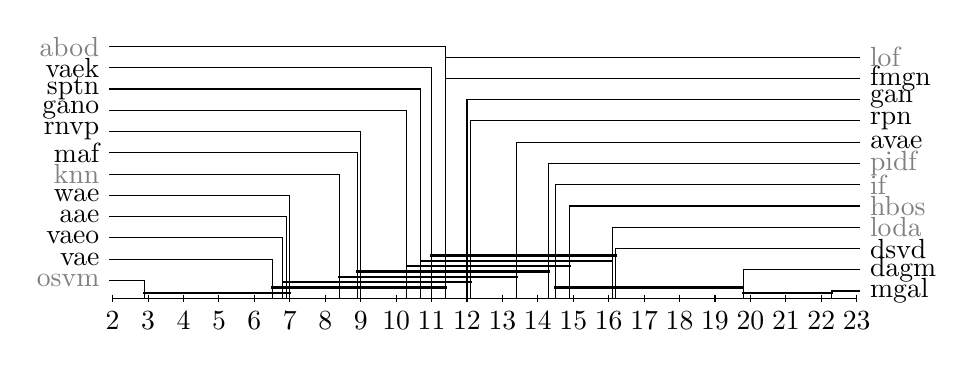
\begin{tikzpicture}[scale=0.45] 
  \draw (2.0,0) -- (23.0,0); 
  \foreach \x in {2,...,23} \draw (\x,0.10) -- (\x,-0.10) node[anchor=north]{$\x$}; 
  \draw (2.9,0) -- (2.9,0.5) -- (1.9, 0.5) node[anchor=east] {\textcolor{gray}{osvm}}; 
  \draw (6.5,0) -- (6.5,1.0999999999999999) -- (1.9, 1.0999999999999999) node[anchor=east] {vae}; 
  \draw (6.8,0) -- (6.8,1.6999999999999997) -- (1.9, 1.6999999999999997) node[anchor=east] {vaeo}; 
  \draw (6.9,0) -- (6.9,2.3) -- (1.9, 2.3) node[anchor=east] {aae}; 
  \draw (7.0,0) -- (7.0,2.9) -- (1.9, 2.9) node[anchor=east] {wae}; 
  \draw (8.4,0) -- (8.4,3.4999999999999996) -- (1.9, 3.4999999999999996) node[anchor=east] {\textcolor{gray}{knn}}; 
  \draw (8.9,0) -- (8.9,4.1000000000000005) -- (1.9, 4.1000000000000005) node[anchor=east] {maf}; 
  \draw (9.0,0) -- (9.0,4.7) -- (1.9, 4.7) node[anchor=east] {rnvp}; 
  \draw (10.3,0) -- (10.3,5.3) -- (1.9, 5.3) node[anchor=east] {gano}; 
  \draw (10.7,0) -- (10.7,5.9) -- (1.9, 5.9) node[anchor=east] {sptn}; 
  \draw (11.0,0) -- (11.0,6.5) -- (1.9, 6.5) node[anchor=east] {vaek}; 
  \draw (11.4,0) -- (11.4,7.1) -- (1.9, 7.1) node[anchor=east] {\textcolor{gray}{abod}}; 
  \draw (11.4,0) -- (11.4,6.8) -- (23.1, 6.8) node[anchor=west] {\textcolor{gray}{lof}}; 
  \draw (11.4,0) -- (11.4,6.2) -- (23.1, 6.2) node[anchor=west] {fmgn}; 
  \draw (12.0,0) -- (12.0,5.6) -- (23.1, 5.6) node[anchor=west] {gan}; 
  \draw (12.1,0) -- (12.1,5.0) -- (23.1, 5.0) node[anchor=west] {rpn}; 
  \draw (13.4,0) -- (13.4,4.4) -- (23.1, 4.4) node[anchor=west] {avae}; 
  \draw (14.3,0) -- (14.3,3.8) -- (23.1, 3.8) node[anchor=west] {\textcolor{gray}{pidf}}; 
  \draw (14.5,0) -- (14.5,3.2) -- (23.1, 3.2) node[anchor=west] {\textcolor{gray}{if}}; 
  \draw (14.9,0) -- (14.9,2.6) -- (23.1, 2.6) node[anchor=west] {\textcolor{gray}{hbos}}; 
  \draw (16.1,0) -- (16.1,1.9999999999999998) -- (23.1, 1.9999999999999998) node[anchor=west] {\textcolor{gray}{loda}}; 
  \draw (16.2,0) -- (16.2,1.4) -- (23.1, 1.4) node[anchor=west] {dsvd}; 
  \draw (19.8,0) -- (19.8,0.8) -- (23.1, 0.8) node[anchor=west] {dagm}; 
  \draw (22.3,0) -- (22.3,0.2) -- (23.1, 0.2) node[anchor=west] {mgal}; 
  \draw[line width=0.03cm,color=black,draw opacity=1.0] (2.87,0.15) -- (7.03,0.15); 
  \draw[line width=0.03cm,color=black,draw opacity=1.0] (6.47,0.3) -- (11.43,0.3); 
  \draw[line width=0.03cm,color=black,draw opacity=1.0] (6.77,0.44999999999999996) -- (12.129999999999999,0.44999999999999996); 
  \draw[line width=0.03cm,color=black,draw opacity=1.0] (8.370000000000001,0.6) -- (13.43,0.6); 
  \draw[line width=0.03cm,color=black,draw opacity=1.0] (8.870000000000001,0.75) -- (14.33,0.75); 
  \draw[line width=0.03cm,color=black,draw opacity=1.0] (10.270000000000001,0.9) -- (14.93,0.9); 
  \draw[line width=0.03cm,color=black,draw opacity=1.0] (10.67,1.05) -- (16.130000000000003,1.05); 
  \draw[line width=0.03cm,color=black,draw opacity=1.0] (10.97,1.2) -- (16.23,1.2); 
  \draw[line width=0.03cm,color=black,draw opacity=1.0] (14.47,0.3) -- (19.830000000000002,0.3); 
  \draw[line width=0.03cm,color=black,draw opacity=1.0] (19.77,0.15) -- (22.330000000000002,0.15); 
 \end{tikzpicture} 
} & \resizebox{\columnwidth}{!}{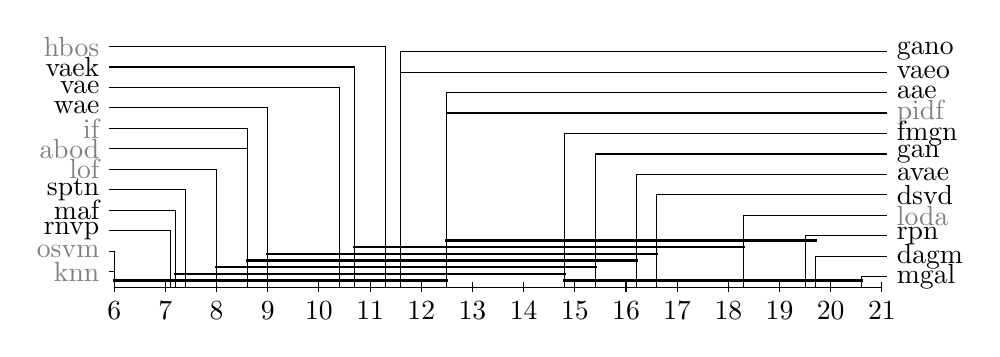
\begin{tikzpicture}[scale=0.65] 
  \draw (6.0,0) -- (21.0,0); 
  \foreach \x in {6,...,21} \draw (\x,0.10) -- (\x,-0.10) node[anchor=north]{$\x$}; 
  \draw (6.0,0) -- (6.0,0.30000000000000004) -- (5.9, 0.30000000000000004) node[anchor=east] {\textcolor{gray}{knn}}; 
  \draw (6.0,0) -- (6.0,0.7000000000000001) -- (5.9, 0.7000000000000001) node[anchor=east] {\textcolor{gray}{osvm}}; 
  \draw (7.1,0) -- (7.1,1.1) -- (5.9, 1.1) node[anchor=east] {rnvp}; 
  \draw (7.2,0) -- (7.2,1.5) -- (5.9, 1.5) node[anchor=east] {maf}; 
  \draw (7.4,0) -- (7.4,1.9) -- (5.9, 1.9) node[anchor=east] {sptn}; 
  \draw (8.0,0) -- (8.0,2.3000000000000003) -- (5.9, 2.3000000000000003) node[anchor=east] {\textcolor{gray}{lof}}; 
  \draw (8.6,0) -- (8.6,2.7) -- (5.9, 2.7) node[anchor=east] {\textcolor{gray}{abod}}; 
  \draw (8.6,0) -- (8.6,3.1) -- (5.9, 3.1) node[anchor=east] {\textcolor{gray}{if}}; 
  \draw (9.0,0) -- (9.0,3.5) -- (5.9, 3.5) node[anchor=east] {wae}; 
  \draw (10.4,0) -- (10.4,3.9) -- (5.9, 3.9) node[anchor=east] {vae}; 
  \draw (10.7,0) -- (10.7,4.300000000000001) -- (5.9, 4.300000000000001) node[anchor=east] {vaek}; 
  \draw (11.3,0) -- (11.3,4.700000000000001) -- (5.9, 4.700000000000001) node[anchor=east] {\textcolor{gray}{hbos}}; 
  \draw (11.6,0) -- (11.6,4.6000000000000005) -- (21.1, 4.6000000000000005) node[anchor=west] {gano}; 
  \draw (11.6,0) -- (11.6,4.2) -- (21.1, 4.2) node[anchor=west] {vaeo}; 
  \draw (12.5,0) -- (12.5,3.8000000000000003) -- (21.1, 3.8000000000000003) node[anchor=west] {aae}; 
  \draw (12.5,0) -- (12.5,3.4000000000000004) -- (21.1, 3.4000000000000004) node[anchor=west] {\textcolor{gray}{pidf}}; 
  \draw (14.8,0) -- (14.8,3.0000000000000004) -- (21.1, 3.0000000000000004) node[anchor=west] {fmgn}; 
  \draw (15.4,0) -- (15.4,2.6000000000000005) -- (21.1, 2.6000000000000005) node[anchor=west] {gan}; 
  \draw (16.2,0) -- (16.2,2.2) -- (21.1, 2.2) node[anchor=west] {avae}; 
  \draw (16.6,0) -- (16.6,1.8) -- (21.1, 1.8) node[anchor=west] {dsvd}; 
  \draw (18.3,0) -- (18.3,1.4000000000000001) -- (21.1, 1.4000000000000001) node[anchor=west] {\textcolor{gray}{loda}}; 
  \draw (19.5,0) -- (19.5,1.0) -- (21.1, 1.0) node[anchor=west] {rpn}; 
  \draw (19.7,0) -- (19.7,0.6000000000000001) -- (21.1, 0.6000000000000001) node[anchor=west] {dagm}; 
  \draw (20.6,0) -- (20.6,0.2) -- (21.1, 0.2) node[anchor=west] {mgal}; 
  \draw[line width=0.03cm,color=black,draw opacity=1.0] (5.97,0.13) -- (12.53,0.13); 
  \draw[line width=0.03cm,color=black,draw opacity=1.0] (7.17,0.26) -- (14.83,0.26); 
  \draw[line width=0.03cm,color=black,draw opacity=1.0] (7.97,0.39) -- (15.43,0.39); 
  \draw[line width=0.03cm,color=black,draw opacity=1.0] (8.57,0.52) -- (16.23,0.52); 
  \draw[line width=0.03cm,color=black,draw opacity=1.0] (8.97,0.65) -- (16.630000000000003,0.65); 
  \draw[line width=0.03cm,color=black,draw opacity=1.0] (10.67,0.78) -- (18.330000000000002,0.78); 
  \draw[line width=0.03cm,color=black,draw opacity=1.0] (12.47,0.91) -- (19.73,0.91); 
  \draw[line width=0.03cm,color=black,draw opacity=1.0] (14.770000000000001,0.13) -- (20.630000000000003,0.13); 
 \end{tikzpicture} 
} \\
    a) tabular datasets, anomaly validation & b) tabular datasets, clean validation \\  
    \resizebox{\columnwidth}{!}{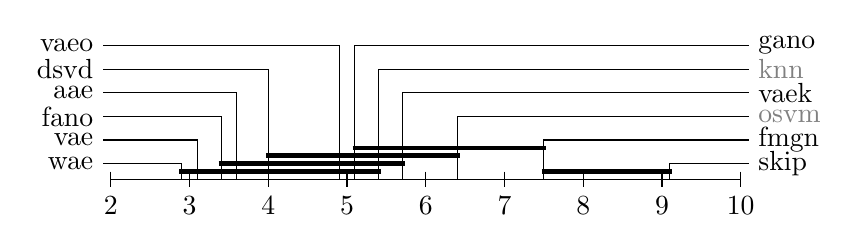
\begin{tikzpicture}[scale=1.0] 
  \draw (2.0,0) -- (10.0,0); 
  \foreach \x in {2,...,10} \draw (\x,0.10) -- (\x,-0.10) node[anchor=north]{$\x$}; 
  \draw (2.9,0) -- (2.9,0.19999999999999998) -- (1.9, 0.19999999999999998) node[anchor=east] {wae}; 
  \draw (3.1,0) -- (3.1,0.5) -- (1.9, 0.5) node[anchor=east] {vae}; 
  \draw (3.4,0) -- (3.4,0.7999999999999999) -- (1.9, 0.7999999999999999) node[anchor=east] {fano}; 
  \draw (3.6,0) -- (3.6,1.0999999999999999) -- (1.9, 1.0999999999999999) node[anchor=east] {aae}; 
  \draw (4.0,0) -- (4.0,1.4) -- (1.9, 1.4) node[anchor=east] {dsvd}; 
  \draw (4.9,0) -- (4.9,1.6999999999999997) -- (1.9, 1.6999999999999997) node[anchor=east] {vaeo}; 
  \draw (5.1,0) -- (5.1,1.7) -- (10.1, 1.7) node[anchor=west] {gano}; 
  \draw (5.4,0) -- (5.4,1.4) -- (10.1, 1.4) node[anchor=west] {\textcolor{gray}{knn}}; 
  \draw (5.7,0) -- (5.7,1.0999999999999999) -- (10.1, 1.0999999999999999) node[anchor=west] {vaek}; 
  \draw (6.4,0) -- (6.4,0.8) -- (10.1, 0.8) node[anchor=west] {\textcolor{gray}{osvm}}; 
  \draw (7.5,0) -- (7.5,0.5) -- (10.1, 0.5) node[anchor=west] {fmgn}; 
  \draw (9.1,0) -- (9.1,0.2) -- (10.1, 0.2) node[anchor=west] {skip}; 
  \draw[line width=0.06cm,color=black,draw opacity=1.0] (2.87,0.1) -- (5.430000000000001,0.1); 
  \draw[line width=0.06cm,color=black,draw opacity=1.0] (3.37,0.2) -- (5.73,0.2); 
  \draw[line width=0.06cm,color=black,draw opacity=1.0] (3.97,0.30000000000000004) -- (6.430000000000001,0.30000000000000004); 
  \draw[line width=0.06cm,color=black,draw opacity=1.0] (5.069999999999999,0.4) -- (7.53,0.4); 
  \draw[line width=0.06cm,color=black,draw opacity=1.0] (7.47,0.1) -- (9.129999999999999,0.1); 
 \end{tikzpicture} 
} & \resizebox{\columnwidth}{!}{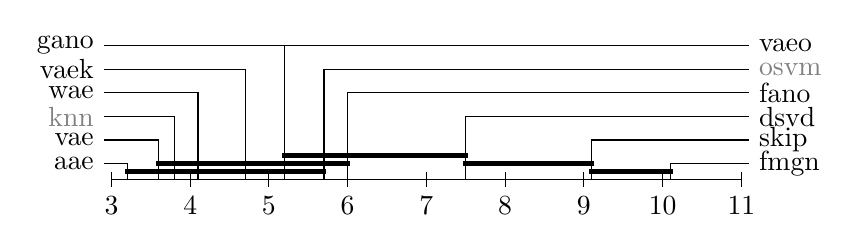
\begin{tikzpicture}[scale=1.0] 
  \draw (3.0,0) -- (11.0,0); 
  \foreach \x in {3,...,11} \draw (\x,0.10) -- (\x,-0.10) node[anchor=north]{$\x$}; 
  \draw (3.2,0) -- (3.2,0.19999999999999998) -- (2.9, 0.19999999999999998) node[anchor=east] {aae}; 
  \draw (3.6,0) -- (3.6,0.5) -- (2.9, 0.5) node[anchor=east] {vae}; 
  \draw (3.8,0) -- (3.8,0.7999999999999999) -- (2.9, 0.7999999999999999) node[anchor=east] {\textcolor{gray}{knn}}; 
  \draw (4.1,0) -- (4.1,1.0999999999999999) -- (2.9, 1.0999999999999999) node[anchor=east] {wae}; 
  \draw (4.7,0) -- (4.7,1.4) -- (2.9, 1.4) node[anchor=east] {vaek}; 
  \draw (5.2,0) -- (5.2,1.6999999999999997) -- (2.9, 1.6999999999999997) node[anchor=east] {gano}; 
  \draw (5.2,0) -- (5.2,1.7) -- (11.1, 1.7) node[anchor=west] {vaeo}; 
  \draw (5.7,0) -- (5.7,1.4) -- (11.1, 1.4) node[anchor=west] {\textcolor{gray}{osvm}}; 
  \draw (6.0,0) -- (6.0,1.0999999999999999) -- (11.1, 1.0999999999999999) node[anchor=west] {fano}; 
  \draw (7.5,0) -- (7.5,0.8) -- (11.1, 0.8) node[anchor=west] {dsvd}; 
  \draw (9.1,0) -- (9.1,0.5) -- (11.1, 0.5) node[anchor=west] {skip}; 
  \draw (10.1,0) -- (10.1,0.2) -- (11.1, 0.2) node[anchor=west] {fmgn}; 
  \draw[line width=0.06cm,color=black,draw opacity=1.0] (3.1700000000000004,0.1) -- (5.73,0.1); 
  \draw[line width=0.06cm,color=black,draw opacity=1.0] (3.5700000000000003,0.2) -- (6.03,0.2); 
  \draw[line width=0.06cm,color=black,draw opacity=1.0] (5.17,0.30000000000000004) -- (7.53,0.30000000000000004); 
  \draw[line width=0.06cm,color=black,draw opacity=1.0] (7.47,0.2) -- (9.129999999999999,0.2); 
  \draw[line width=0.06cm,color=black,draw opacity=1.0] (9.07,0.1) -- (10.129999999999999,0.1); 
 \end{tikzpicture} 
}\\
    c) statistical image datasets, anomaly validation & d) statistical image  datasets, clean validation \\ 
     \resizebox{\columnwidth}{!}{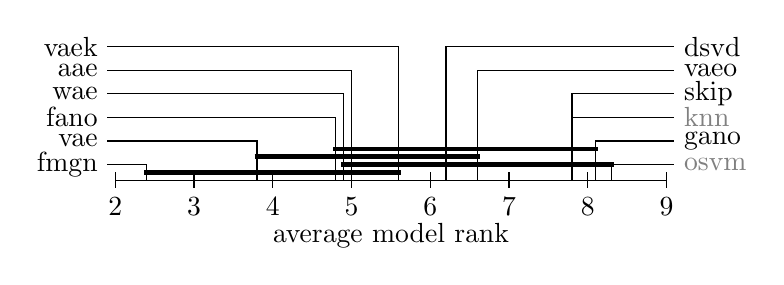
\begin{tikzpicture}[scale=1.0] 
  \draw (2.0,0) -- (9.0,0); 
  \foreach \x in {2,...,9} \draw (\x,0.10) -- (\x,-0.10) node[anchor=north]{$\x$}; 
  \draw (2.4,0) -- (2.4,0.19999999999999998) -- (1.9, 0.19999999999999998) node[anchor=east] {fmgn}; 
  \draw (3.8,0) -- (3.8,0.5) -- (1.9, 0.5) node[anchor=east] {vae}; 
  \draw (4.8,0) -- (4.8,0.7999999999999999) -- (1.9, 0.7999999999999999) node[anchor=east] {fano}; 
  \draw (4.9,0) -- (4.9,1.0999999999999999) -- (1.9, 1.0999999999999999) node[anchor=east] {wae}; 
  \draw (5.0,0) -- (5.0,1.4) -- (1.9, 1.4) node[anchor=east] {aae}; 
  \draw (5.6,0) -- (5.6,1.6999999999999997) -- (1.9, 1.6999999999999997) node[anchor=east] {vaek}; 
  \draw (6.2,0) -- (6.2,1.7) -- (9.1, 1.7) node[anchor=west] {dsvd}; 
  \draw (6.6,0) -- (6.6,1.4) -- (9.1, 1.4) node[anchor=west] {vaeo}; 
  \draw (7.8,0) -- (7.8,1.0999999999999999) -- (9.1, 1.0999999999999999) node[anchor=west] {skip}; 
  \draw (7.8,0) -- (7.8,0.8) -- (9.1, 0.8) node[anchor=west] {\textcolor{gray}{knn}}; 
  \draw (8.1,0) -- (8.1,0.5) -- (9.1, 0.5) node[anchor=west] {gano}; 
  \draw (8.3,0) -- (8.3,0.2) -- (9.1, 0.2) node[anchor=west] {\textcolor{gray}{osvm}}; 
  \draw[line width=0.06cm,color=black,draw opacity=1.0] (2.37,0.1) -- (5.63,0.1); 
  \draw[line width=0.06cm,color=black,draw opacity=1.0] (3.77,0.3) -- (6.63,0.3); 
  \draw[line width=0.06cm,color=black,draw opacity=1.0] (4.77,0.4) -- (8.129999999999999,0.4); 
  \draw[line width=0.06cm,color=black,draw opacity=1.0] (4.87,0.2) -- (8.33,0.2); 
  \node[anchor=center] at (5.5,-0.7) {average model rank};
 \end{tikzpicture} 
} & \resizebox{\columnwidth}{!}{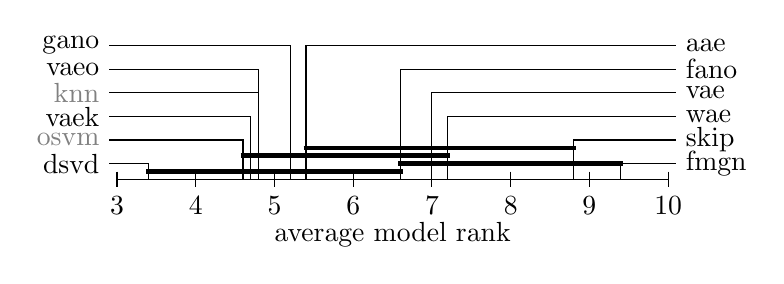
\begin{tikzpicture}[scale=1.0] 
  \draw (3.0,0) -- (10.0,0); 
  \foreach \x in {3,...,10} \draw (\x,0.10) -- (\x,-0.10) node[anchor=north]{$\x$}; 
  \draw (3.4,0) -- (3.4,0.19999999999999998) -- (2.9, 0.19999999999999998) node[anchor=east] {dsvd}; 
  \draw (4.6,0) -- (4.6,0.5) -- (2.9, 0.5) node[anchor=east] {\textcolor{gray}{osvm}}; 
  \draw (4.7,0) -- (4.7,0.7999999999999999) -- (2.9, 0.7999999999999999) node[anchor=east] {vaek}; 
  \draw (4.8,0) -- (4.8,1.0999999999999999) -- (2.9, 1.0999999999999999) node[anchor=east] {\textcolor{gray}{knn}}; 
  \draw (4.8,0) -- (4.8,1.4) -- (2.9, 1.4) node[anchor=east] {vaeo}; 
  \draw (5.2,0) -- (5.2,1.6999999999999997) -- (2.9, 1.6999999999999997) node[anchor=east] {gano}; 
  \draw (5.4,0) -- (5.4,1.7) -- (10.1, 1.7) node[anchor=west] {aae}; 
  \draw (6.6,0) -- (6.6,1.4) -- (10.1, 1.4) node[anchor=west] {fano}; 
  \draw (7.0,0) -- (7.0,1.0999999999999999) -- (10.1, 1.0999999999999999) node[anchor=west] {vae}; 
  \draw (7.2,0) -- (7.2,0.8) -- (10.1, 0.8) node[anchor=west] {wae}; 
  \draw (8.8,0) -- (8.8,0.5) -- (10.1, 0.5) node[anchor=west] {skip}; 
  \draw (9.4,0) -- (9.4,0.2) -- (10.1, 0.2) node[anchor=west] {fmgn}; 
  \draw[line width=0.06cm,color=black,draw opacity=1.0] (3.37,0.1) -- (6.63,0.1); 
  \draw[line width=0.06cm,color=black,draw opacity=1.0] (4.569999999999999,0.3) -- (7.23,0.3); 
  \draw[line width=0.06cm,color=black,draw opacity=1.0] (5.37,0.4) -- (8.83,0.4); 
  \draw[line width=0.06cm,color=black,draw opacity=1.0] (6.569999999999999,0.2) -- (9.43,0.2); 
  \node[anchor=center] at (6.5,-0.7) {average model rank};
 \end{tikzpicture} 
} \\
    e) semantic image  datasets, anomaly validation & f) semantic image datasets, clean validation \\
    \end{tabular}
 \caption{Critical difference diagram of models ranked via the test AUC. Models whose performance is statistically indistinguishable have a difference of ranks under the critical value of the Nemenyi test $CD_{0.1}$ and are joined by a horizontal band. Results are presented for different types of datasets: tabular (Top row), image datasets with statistical anomalies (Middle row), and image datasets with semantic anomalies (Bottom row); and two different hyperparameter selection cases: using anomalies in validation (left) and using clean validation (right).
 }
 % $CD_{0.05}(24, 40) = 5.75$
 \label{fig:critical_diag}
\end{figure*}

\subsection{Dataset context}
\label{sec:dataset_context}
The results of experimental comparison on all dataset types are presented in the form of critical difference diagrams (CDD) as recommended by Dem\v{s}ar~\cite{demvsar2006statistical}, are in Fig.~\ref{fig:critical_diag}. Diagrams show the average rank of detectors across the datasets together with a confidence band that indicates that a statistical test cannot reject the hypothesis that two detectors perform the same. The underlying  AUC values on the testing set for all individual datasets are given in Tab.~\ref{tab:tabular_anomalies}, \ref{tab:tabular_clean}, \ref{tab:images_stat_auc_auc_combined}, and~\ref{tab:images_semantic_auc_auc_combined}. We now comment on the influence of the datatype with respect to two types of hyperparameter selection strategies differing in the number of anomalies in the validation set as defined in Section~\ref{sec:contexts}: i) anomaly validation context, and ii) clean validation context.

\emph{Tabular data:} OC-SVM works the best and it is \emph{statistically better} than almost all detectors except autoencoder-based generative models and VAE combined with OC-SVM in the case of anomaly validation context. The first 11 places (roughly one half) belong to models that can be divided into three groups: (i) OC-SVM and its variants, which estimate a density level of a distribution; (ii) flow models and kNN, which estimate the pdf (un-normalized in case of kNN); (iii) and variants of auto-encoders, where reconstruction error is related to pdf as explained in~\cite{vsmidl2019anomaly}. The same types of methods occupy the top positions in the clean validation context, Fig.~\ref{fig:critical_diag}b), however in a different order. The best is the kNN, and all other pdf-modeling methods (flows) have improved relative to the anomaly validation context. The autoencoder-based methods moved beyond classical methods (LOF, ABOD, IF). We believe that models in the lower half of the scale in both validation contexts are not suitable for detecting statistical anomalies. We cannot explain the poor performance of MOGAAL, DAGMM, and adVAE,\footnote{We have contacted the author of pyOD from wherein we took the implementation of MOGAAL, and we were assured that his implementation is a copy of that provided by the authors. Therefore, we consider the implementation to be correct.} and we attribute it to different experimental environment. DeepSVDD was primarily implemented for image problems, where it performs relatively well.

Moreover, differences in mean ranks of many models in Fig.~\ref{fig:critical_diag} are statistically insignificant at level $p=0.1$, which is disappointing. Assuming the ranks remain the same, another 51 datasets would be needed to make the difference between OC-SVM and VAE statistically significant on tabular data with 50\% anomalies. This indicates that the results are still noisy and can be easily changed for a different choice of datasets.

\emph{Statistical image data:} WAE and VAE models have the best average rank when evaluated on statistical image data, although their lead is not statistically significant over most of the other models as is evident from Fig.~\ref{fig:critical_diag}c). The autoencoder-based methods (AAE,VAE,WAE) perform well also in the clean validation context, complemented by kNN, Fig.~\ref{fig:critical_diag}d).

\emph{Semantic image data}
A different story is told by Fig.~\ref{fig:critical_diag}e) where the ranking of methods on image datasets with semantic anomalies is dominated by fmGAN by a large margin in the anomaly validation context. However, it is also the worst method in the clean validation context. In an opposite manner, 
OC-SVM and kNN perform very poorly in the anomaly validation context, but they are among the best in the clean validation context.  The best performing method in the clean validation context is DeepSVDD~\cite{ruff2018deep}. We conjecture that the performance of the fmGAN is related to the variability of its training. With a sufficient number of anomalies in the validation set, it is possible to find one trained model that fits the problem.

The typical anomalies detected by various methods on image datasets are provided in the Supplementary \ref{sec:appendix_extending_image_results}.


\subsection{Hyperparameter selection context}
\label{sec:hyperparameter_context}
The influence of the hyperparameter selection procedure on the results in the previous section is now studied in detail for few selected methods. We choose only those that scored among the best in the previous section. First, we analyze the sensitivity of these methods to the number of anomalies in the validation set. Second, we study hyperparameter selection for two individual methods, variational autoencoder family and OC-SVM.

\subsubsection{Impact of the number of anomalies in the validation set}
\begin{figure*}[hbt!]
    \centering
    % \footnotesize
    % \resizebox {\linewidth}{!}{
    % \input{data/chapter_comparison/combined_knowledge_rank_pat_auc_repre_mvc}
    % \input{data/chapter_comparison/combined_knowledge_rank_pat_auc_repre_mvc_per_ac}
    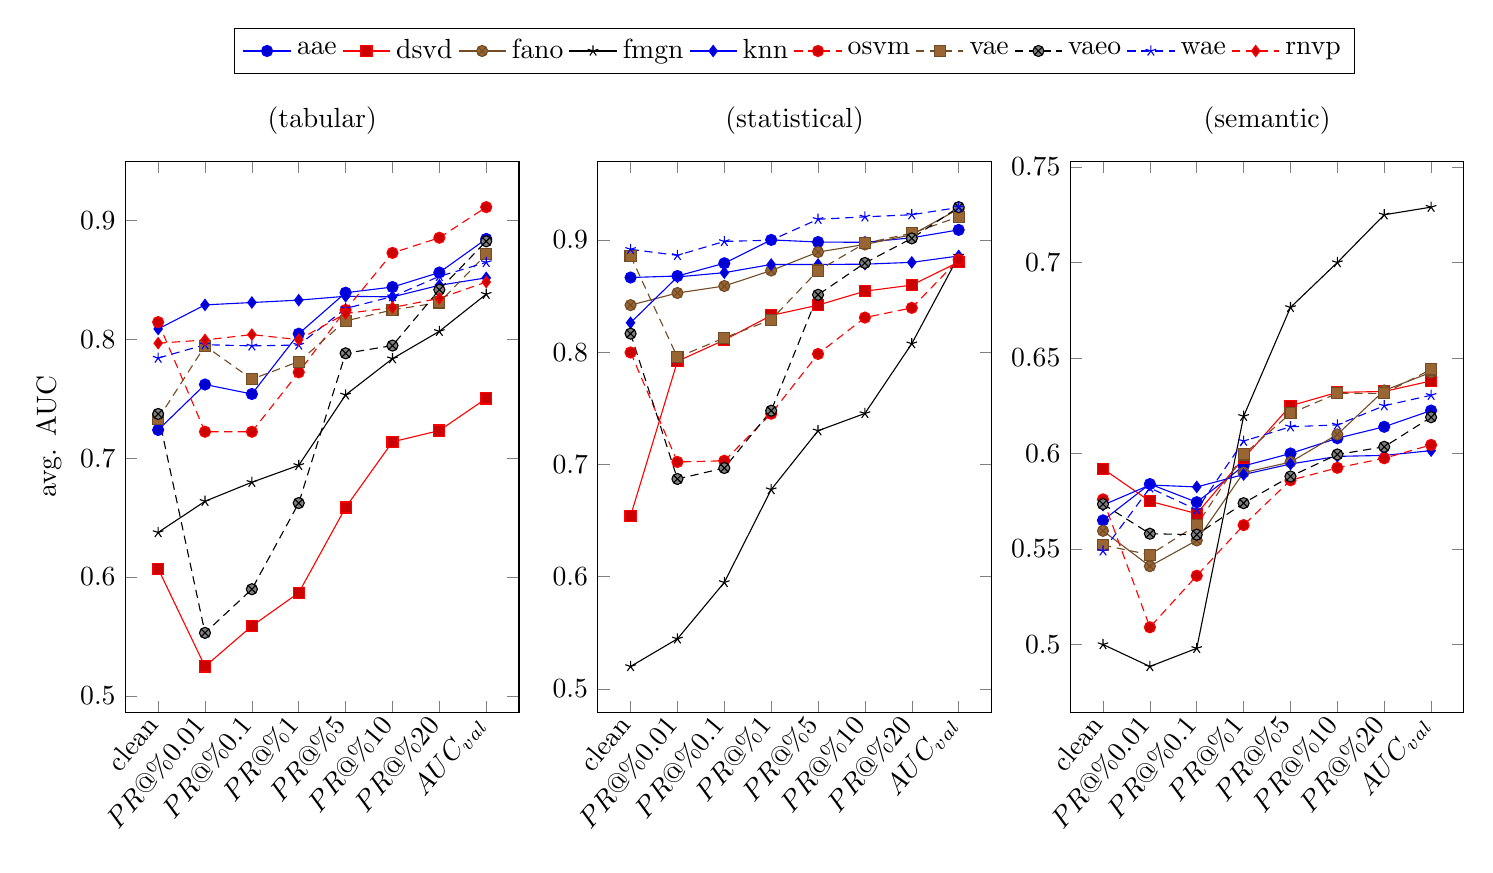
\begin{tikzpicture}[]
\begin{groupplot}[group style={vertical sep = 0.5cm, horizontal sep = 1.0cm, group size=3 by 1}]

\nextgroupplot [
  % legend style = {at={(0.3,1.30)}, anchor=west},
  ylabel = {avg. AUC},
  width=5cm, height=7cm, scale only axis=true, 
  xtick={1,2,3,4,5,6,7,8}, 
  xticklabels={clean,$PR@\%0.01$,$PR@\%0.1$,$PR@\%1$,$PR@\%5$,$PR@\%10$,$PR@\%20$,$AUC_{val}$},
  width=5cm, height=7cm, scale only axis=true,
  x tick label style={rotate=50,anchor=east},
  title = {(tabular)},
  % title style={at={(current bounding box.north)}, anchor=west},
]

\addplot+ coordinates {
  (1.0, 0.72375)
  (2.0, 0.762)
  (3.0, 0.754)
  (4.0, 0.8047500000000001)
  (5.0, 0.83925)
  (6.0, 0.844)
  (7.0, 0.8562500000000002)
  (8.0, 0.8845000000000001)
};

\addplot+ coordinates {
  (1.0, 0.607)
  (2.0, 0.52475)
  (3.0, 0.5587500000000001)
  (4.0, 0.5867500000000001)
  (5.0, 0.6585)
  (6.0, 0.71375)
  (7.0, 0.7232500000000001)
  (8.0, 0.7502500000000001)
};

\addplot+ coordinates {};

\addplot+ coordinates {
  (1.0, 0.6375)
  (2.0, 0.66375)
  (3.0, 0.6797500000000001)
  (4.0, 0.6940000000000001)
  (5.0, 0.75325)
  (6.0, 0.7837500000000001)
  (7.0, 0.8067500000000001)
  (8.0, 0.8380000000000001)
};

\addplot+ coordinates {
  (1.0, 0.8087500000000002)
  (2.0, 0.8290000000000001)
  (3.0, 0.8310000000000001)
  (4.0, 0.8329999999999999)
  (5.0, 0.8362499999999999)
  (6.0, 0.8357499999999998)
  (7.0, 0.8454999999999998)
  (8.0, 0.8517499999999998)
};

\addplot+ coordinates {
  (1.0, 0.8145)
  (2.0, 0.7222500000000001)
  (3.0, 0.7222500000000001)
  (4.0, 0.77225)
  (5.0, 0.8247500000000001)
  (6.0, 0.8727499999999999)
  (7.0, 0.8854999999999998)
  (8.0, 0.9112500000000001)
};

\addplot+ coordinates {
  (1.0, 0.7329999999999999)
  (2.0, 0.7945)
  (3.0, 0.7665)
  (4.0, 0.7812500000000001)
  (5.0, 0.8154999999999999)
  (6.0, 0.8247499999999999)
  (7.0, 0.8310000000000001)
  (8.0, 0.8714999999999999)
};

\addplot+ coordinates {
  (1.0, 0.7372500000000001)
  (2.0, 0.5530000000000002)
  (3.0, 0.5897500000000002)
  (4.0, 0.6622499999999999)
  (5.0, 0.7882499999999999)
  (6.0, 0.79475)
  (7.0, 0.84175)
  (8.0, 0.8825)
};

\addplot+ coordinates {
  (1.0, 0.7842499999999999)
  (2.0, 0.7955000000000002)
  (3.0, 0.7945)
  (4.0, 0.79525)
  (5.0, 0.826)
  (6.0, 0.836)
  (7.0, 0.853)
  (8.0, 0.8647499999999999)
};

\addplot+ coordinates {
  (1.0, 0.7967500000000001)
  (2.0, 0.7994999999999999)
  (3.0, 0.8039999999999999)
  (4.0, 0.7997500000000002)
  (5.0, 0.8217500000000001)
  (6.0, 0.82675)
  (7.0, 0.8344999999999999)
  (8.0, 0.8482500000000002)
};

% \legend{{}{aae}, {}{dsvd}, {}{fmgn}, {}{knn}, {}{osvm}, {}{vae}, {}{vaeo}, {}{wae}, {}{rnvp}}

\nextgroupplot [
  legend columns = -1,
  legend style = {at={(0.5,1.2)}, anchor=center},
  legend entries = {aae, dsvd, fano, fmgn, knn, osvm, vae, vaeo, wae, rnvp},
  width=5cm, height=7cm, scale only axis=true, 
  xtick={1,2,3,4,5,6,7,8}, 
  xticklabels={clean,$PR@\%0.01$,$PR@\%0.1$,$PR@\%1$,$PR@\%5$,$PR@\%10$,$PR@\%20$,$AUC_{val}$},
  width=5cm, height=7cm, scale only axis=true,
  x tick label style={rotate=50,anchor=east},
  title = {(statistical)},
  % title style={at={(current bounding box.north)}, anchor=west},
]

\addplot+ coordinates {
  (1.0, 0.8664864864864865)
  (2.0, 0.867837837837838)
  (3.0, 0.8791891891891892)
  (4.0, 0.8999999999999999)
  (5.0, 0.8981081081081083)
  (6.0, 0.8978378378378378)
  (7.0, 0.901891891891892)
  (8.0, 0.908918918918919)
};

\addplot+ coordinates {
  (1.0, 0.654054054054054)
  (2.0, 0.7918918918918918)
  (3.0, 0.8108108108108109)
  (4.0, 0.8327027027027026)
  (5.0, 0.841891891891892)
  (6.0, 0.8543243243243243)
  (7.0, 0.8597297297297297)
  (8.0, 0.8802702702702703)
};

\addplot+ coordinates {
  (1.0, 0.841891891891892)
  (2.0, 0.8527027027027027)
  (3.0, 0.8589189189189189)
  (4.0, 0.8727027027027027)
  (5.0, 0.8891891891891893)
  (6.0, 0.8959459459459459)
  (7.0, 0.9045945945945946)
  (8.0, 0.9275675675675675)
};

\addplot+ coordinates {
  (1.0, 0.5199999999999999)
  (2.0, 0.5445945945945946)
  (3.0, 0.5948648648648649)
  (4.0, 0.6775675675675675)
  (5.0, 0.73)
  (6.0, 0.7454054054054053)
  (7.0, 0.8075675675675675)
  (8.0, 0.8856756756756757)
};

\addplot+ coordinates {
  (1.0, 0.8262162162162162)
  (2.0, 0.8670270270270269)
  (3.0, 0.8708108108108108)
  (4.0, 0.8781081081081081)
  (5.0, 0.8781081081081081)
  (6.0, 0.8783783783783784)
  (7.0, 0.8799999999999999)
  (8.0, 0.8856756756756757)
};

\addplot+ coordinates {
  (1.0, 0.7997297297297298)
  (2.0, 0.7021621621621621)
  (3.0, 0.7032432432432432)
  (4.0, 0.7451351351351351)
  (5.0, 0.7983783783783783)
  (6.0, 0.8308108108108109)
  (7.0, 0.8394594594594594)
  (8.0, 0.8824324324324324)
};

\addplot+ coordinates {
  (1.0, 0.8856756756756757)
  (2.0, 0.7954054054054054)
  (3.0, 0.8127027027027027)
  (4.0, 0.828918918918919)
  (5.0, 0.8727027027027027)
  (6.0, 0.897027027027027)
  (7.0, 0.905945945945946)
  (8.0, 0.9205405405405408)
};

\addplot+ coordinates {
  (1.0, 0.8164864864864865)
  (2.0, 0.687027027027027)
  (3.0, 0.6967567567567567)
  (4.0, 0.7478378378378379)
  (5.0, 0.851081081081081)
  (6.0, 0.8794594594594595)
  (7.0, 0.9013513513513514)
  (8.0, 0.929189189189189)
};

\addplot+ coordinates {
  (1.0, 0.8916216216216215)
  (2.0, 0.8862162162162162)
  (3.0, 0.8986486486486487)
  (4.0, 0.8997297297297298)
  (5.0, 0.9183783783783783)
  (6.0, 0.9205405405405406)
  (7.0, 0.9224324324324323)
  (8.0, 0.9289189189189189)
};

% has to be set manually to match the marker style of the flow (9th in the entries bellow)
\addlegendimage{red,densely dashed,every mark/.append style={solid,fill=red!80!black},mark=diamond*} 
% \legend{{}{aae}, {}{dsvd}, {}{fano}, {}{fmgn}, {}{knn}, {}{osvm}, {}{vae}, {}{vaeo}, {}{wae}}

%%% the color 
% blue,every mark/.append style={fill=blue!80!black},mark=*\\
% red,every mark/.append style={fill=red!80!black},mark=square*\\
% brown!60!black,every mark/.append style={fill=brown!80!black},mark=otimes*\\
% black,mark=star\\
% blue,every mark/.append style={fill=blue!80!black},mark=diamond*\\
% red,densely dashed,every mark/.append style={solid,fill=red!80!black},mark=*\\
% brown!60!black,densely dashed,every mark/.append style={
% solid,fill=brown!80!black},mark=square*\\
% black,densely dashed,every mark/.append style={solid,fill=gray},mark=otimes*\\
% blue,densely dashed,mark=star,every mark/.append style=solid\\
% red,densely dashed,every mark/.append style={solid,fill=red!80!black},mark=diamond*\\

\nextgroupplot [
  % legend style = {at={(0.3,1.30)}, anchor=west},
  width=5cm, height=7cm, scale only axis=true, 
  xtick={1,2,3,4,5,6,7,8}, 
  xticklabels={clean,$PR@\%0.01$,$PR@\%0.1$,$PR@\%1$,$PR@\%5$,$PR@\%10$,$PR@\%20$,$AUC_{val}$},
  width=5cm, height=7cm, scale only axis=true,
  x tick label style={rotate=50,anchor=east},
  title = {(semantic)},
  % title style={at={(current bounding box.north)}, anchor=west},
]

\addplot+ coordinates {
  (1.0, 0.5649999999999998)
  (2.0, 0.584)
  (3.0, 0.5745000000000001)
  (4.0, 0.5934999999999999)
  (5.0, 0.6)
  (6.0, 0.6079999999999999)
  (7.0, 0.614)
  (8.0, 0.6224999999999999)
};

\addplot+ coordinates {
  (1.0, 0.5920000000000001)
  (2.0, 0.575)
  (3.0, 0.5685)
  (4.0, 0.5975000000000001)
  (5.0, 0.6250000000000001)
  (6.0, 0.6320000000000001)
  (7.0, 0.6325000000000001)
  (8.0, 0.638)
};

\addplot+ coordinates {
  (1.0, 0.5595000000000001)
  (2.0, 0.541)
  (3.0, 0.5544999999999999)
  (4.0, 0.5899999999999999)
  (5.0, 0.5955)
  (6.0, 0.61)
  (7.0, 0.633)
  (8.0, 0.6424999999999998)
};

\addplot+ coordinates {
  (1.0, 0.5)
  (2.0, 0.4885)
  (3.0, 0.49799999999999994)
  (4.0, 0.6194999999999999)
  (5.0, 0.6765)
  (6.0, 0.7)
  (7.0, 0.7249999999999999)
  (8.0, 0.729)
};

\addplot+ coordinates {
  (1.0, 0.5730000000000001)
  (2.0, 0.5834999999999999)
  (3.0, 0.5824999999999999)
  (4.0, 0.5890000000000001)
  (5.0, 0.5945)
  (6.0, 0.5985)
  (7.0, 0.599)
  (8.0, 0.6015)
};

\addplot+ coordinates {
  (1.0, 0.5760000000000001)
  (2.0, 0.5090000000000001)
  (3.0, 0.536)
  (4.0, 0.5625)
  (5.0, 0.5860000000000001)
  (6.0, 0.5925)
  (7.0, 0.5975000000000001)
  (8.0, 0.6045)
};

\addplot+ coordinates {
  (1.0, 0.552)
  (2.0, 0.5469999999999999)
  (3.0, 0.5625)
  (4.0, 0.5995000000000001)
  (5.0, 0.6210000000000002)
  (6.0, 0.6315000000000001)
  (7.0, 0.6315)
  (8.0, 0.6439999999999999)
};

\addplot+ coordinates {
  (1.0, 0.5735000000000001)
  (2.0, 0.558)
  (3.0, 0.5574999999999999)
  (4.0, 0.574)
  (5.0, 0.588)
  (6.0, 0.5994999999999999)
  (7.0, 0.6035000000000001)
  (8.0, 0.619)
};

\addplot+ coordinates {
  (1.0, 0.549)
  (2.0, 0.5820000000000002)
  (3.0, 0.5705)
  (4.0, 0.6065)
  (5.0, 0.614)
  (6.0, 0.615)
  (7.0, 0.625)
  (8.0, 0.6305)
};

\end{groupplot}

\end{tikzpicture}

    % }
    \caption{Sensitivity of methods to the number of anomalies available in the validation set for hyperparameter selection visualized in terms of the achieved AUC aggregated over all datasets in each category (columns). The clean validation context is the left-most point on the x-axis, and the anomaly validation context (50\% of available anomalies) is the right-most point. The points in-between were obtained by selecting models with the highest precision on the reported portion (e.g. 5\%) of validation samples with the highest anomaly scores.} 
    \label{fig:combined_knowledge_rank_patn_auc_repre}
\end{figure*}

The process of hyperparameter selection described in Sec.~\ref{sub:hyperparameteroptimization} depends on the availability of examples of anomalies in the validation set (recall that it is assumed that the validation dataset does not contain unknown anomalous samples, i.e. is not contaminated). 
Fig.~\ref{fig:combined_knowledge_rank_patn_auc_repre} displays the influence of the number of anomalous samples in the validation set on a finer grid between the two contexts reported before.  Note that for the first point on the x-axis, \textit{clean}, the mechanism of model selection was different from the rest of the graph, as noted in Sec.~\ref{sub:hyperparameteroptimization}. This is the reason for the significant difference between the clean context and the remaining points.

First, we observe that the quality of the models selected using anomalies improves with an increasing number of anomalous samples which is expected. However, for a low number of anomalies, many methods perform significantly worse than in the case of the clean validation context. This behavior is notable across dataset types, especially for OC-SVM, and to some extent VAE. We conjecture that the hyperparameter selection procedure of those methods has a tendency to overfit, and its hyperparameters are not robust. In contrast to this, the performance of kNN, WAE, and RealNVP degrades slowly with the declining number of anomalies, which suggests that they are quite robust in difficult operating conditions. We attribute it to the fact that these methods are more exact in their estimation of data likelihood than the rest. 

Second, we notice that the experimental results on the semantic image datasets are generally poor, as the AUC of the best model (fmGAN) on CIFAR10 is 0.72 and similarly on SVHN2, where the best model achieved $0.74$. On the other hand, anomaly detection methods perform well on statistical image datasets. This indicates, contrary to popular belief that the models fail to learn or identify the important semantic information, or they consider different semantic information anomalous, and they should be told \emph{which} semantic aspect of an image should be considered as an anomaly, as for example blurred images might be anomalous as well.

Results of the same study for individual image datasets are presented in the Supplementary, Fig.~\ref{fig:image_knowledge_rank_pat_auc}. We also provide an illustration of what images were identified as normal and anomalous for the tested methods, Supplementary~\ref{sec:appendix_extending_image_results}.

A practitioner might also desire a method robust with respect to a poor choice of hyperparameters.  In general, deep methods in our experiments have demonstrated higher variance, probably due to the large number of hyperparameters and stochasticity involved in their initialization and training via batched gradient optimization. In this respect, GAN-based models seem to be the least robust, which is in line with~\cite{deecke2018image} stating that GANs are not directly optimized for anomaly detection. This hints at the potential cost of hyperparameter optimization --- with higher performance variance, one is less likely to train a well-performing model in a given number of attempts. 

\subsubsection{Sensitivity Analysis of the VAE family}
\label{sec:vae_results}
Autoencoder-based methods form a whole family with multiple sources of variability, as identified in Sec.~\ref{sec:ae_theory} to be: i) approximation of the likelihood in training (loss function), ii) the richness of latent prior, and iii) the anomaly score. We will analyze the sensitivity of the results to these choices on tabular data in the anomaly validation context. We focus on this family since most of the novel deep generative models for anomaly detection are based on the autoencoder architecture. Additional degrees of freedom include the parametrization of variance of $p_{\vec{\theta}}(\vec{x}|\vec{z}),$ which could be either fixed (called VAE-constant), used in~\cite{yaoUnsupervisedAnomalyDetection2019, wang2020advae, ahnDeepGenerativeModelsBased2020}, scalar (called VAE-scalar), or full diagonal (called VAE-diagonal), used in~\cite{an2015variational,xu2018unsupervised, zenatiEfficientGANBasedAnomaly2018}. In the experiments, all three variations were tested on tabular data; however on image data, the full diagonal was skipped due to computational constraints (and in line with the prior art, where only fixed variance is used).

The overall comparison in Fig.~\ref{fig:critical_diag} revealed that WAE and vanilla VAE variants perform best. The other degrees of freedom, namely richness of prior, used anomaly score, and parametrization of variance, were treated as hyperparameters. Fig.~\ref{fig:tabular_ae_only_box_auc_meanmax} extends the study by showing the distribution of ranks over tabular datasets for different variants of VAE, including GANomaly and adVAE.

First, notice that the spread of the method's ranks over various datasets is significant, as even ranks of the best methods vary from 3 to 15. This means that the conclusions below need to be taken with a grain of salt, as the experimental results are extremely noisy.

The ELBO-based score,  -el, together with the orthogonal decomposition of the likelihood~\cite{pidhorskyi2018generative}, -jc, does not perform well. The sampled reconstruction error (an MC estimate of~\eqref{eq:score_sample}, \mbox{-rs}, almost always performs better than the usual reconstruction error, -rm, calculated according to~\eqref{eq:score_mean}. This demonstrates that the common approach of replacing the mean of the decoder with that of the encoder is inferior but computationally cheaper (see Tab.~\ref{tab:predict_times} with prediction times). The discriminator score~\eqref{eq:disc_score}, -di, of AAE (an autoencoder combined with GAN) seems to be also on par with the MC estimate~\eqref{eq:score_sample}. 

From the same figure, we also conclude that the models modelling full diagonal in $p_{\vec{\theta}}(\vec{x}|\vec{z})$, -d-, seem to be better than the scalar, -s-, or constant, -c-, variants. This result is important, as many comparisons in the prior art use the VAE-constant, despite the version with full diagonal being discussed in the original publication~\cite{kingma2013auto}.

The rich prior distribution on the latent space proposed in \cite{tomczak2018vae}, VAMP, -v-, does not seem to give an advantage in the anomaly detection except in the AAE. Similarly, recent variants adVAE and GANomaly do not seem to work well on the tabular data, but they were not evaluated on them in the original publications.

\begin{figure}
    \centering
    \small
    % \input{data/chapter_comparison/tabular_ae_only_box_auc_meanmax}
    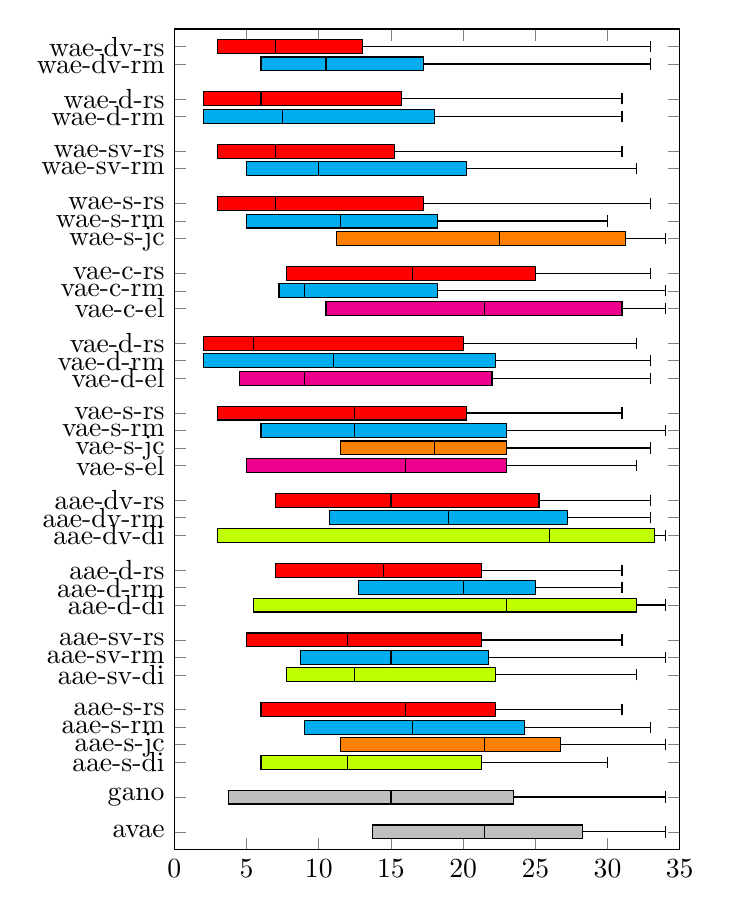
\begin{tikzpicture}
\begin{axis}[
	height=12cm,
	width=8cm,
	ymin=0, ymax=47,
	xmin=0, xmax=35,
	ytick={1,3,5,6,7,8,10,11,12,14,15,16,18,19,20,22,23,24,25,27,28,29,31,32,33,35,36,37,39,40,42,43,45,46},
	yticklabels={avae,gano,aae-s-di,aae-s-jc,aae-s-rm,aae-s-rs,aae-sv-di,aae-sv-rm,aae-sv-rs,aae-d-di,aae-d-rm,aae-d-rs,aae-dv-di,aae-dv-rm,aae-dv-rs,vae-s-el,vae-s-jc,vae-s-rm,vae-s-rs,vae-d-el,vae-d-rm,vae-d-rs,vae-c-el,vae-c-rm,vae-c-rs,wae-s-jc,wae-s-rm,wae-s-rs,wae-sv-rm,wae-sv-rs,wae-d-rm,wae-d-rs,wae-dv-rm,wae-dv-rs}
	]
\addplot [fill=lightgray, boxplot prepared={
draw position=1,
lower whisker=34, lower quartile=13.75,
median=21.5, upper quartile=28.25,
upper whisker=34},
] coordinates {};
\addplot [fill=lightgray, boxplot prepared={
draw position=3,
lower whisker=34, lower quartile=3.75,
median=15.0, upper quartile=23.5,
upper whisker=34},
] coordinates {};
\addplot [fill=lime, boxplot prepared={
draw position=5,
lower whisker=30, lower quartile=6.0,
median=12.0, upper quartile=21.25,
upper whisker=30},
] coordinates {};
\addplot [fill=orange, boxplot prepared={
draw position=6,
lower whisker=34, lower quartile=11.5,
median=21.5, upper quartile=26.75,
upper whisker=34},
] coordinates {};
\addplot [fill=cyan, boxplot prepared={
draw position=7,
lower whisker=33, lower quartile=9.0,
median=16.5, upper quartile=24.25,
upper whisker=33},
] coordinates {};
\addplot [fill=red, boxplot prepared={
draw position=8,
lower whisker=31, lower quartile=6.0,
median=16.0, upper quartile=22.25,
upper whisker=31},
] coordinates {};
\addplot [fill=lime, boxplot prepared={
draw position=10,
lower whisker=32, lower quartile=7.75,
median=12.5, upper quartile=22.25,
upper whisker=32},
] coordinates {};
\addplot [fill=cyan, boxplot prepared={
draw position=11,
lower whisker=34, lower quartile=8.75,
median=15.0, upper quartile=21.75,
upper whisker=34},
] coordinates {};
\addplot [fill=red, boxplot prepared={
draw position=12,
lower whisker=31, lower quartile=5.0,
median=12.0, upper quartile=21.25,
upper whisker=31},
] coordinates {};
\addplot [fill=lime, boxplot prepared={
draw position=14,
lower whisker=34, lower quartile=5.5,
median=23.0, upper quartile=32.0,
upper whisker=34},
] coordinates {};
\addplot [fill=cyan, boxplot prepared={
draw position=15,
lower whisker=31, lower quartile=12.75,
median=20.0, upper quartile=25.0,
upper whisker=31},
] coordinates {};
\addplot [fill=red, boxplot prepared={
draw position=16,
lower whisker=31, lower quartile=7.0,
median=14.5, upper quartile=21.25,
upper whisker=31},
] coordinates {};
\addplot [fill=lime, boxplot prepared={
draw position=18,
lower whisker=34, lower quartile=3.0,
median=26.0, upper quartile=33.25,
upper whisker=34},
] coordinates {};
\addplot [fill=cyan, boxplot prepared={
draw position=19,
lower whisker=33, lower quartile=10.75,
median=19.0, upper quartile=27.25,
upper whisker=33},
] coordinates {};
\addplot [fill=red, boxplot prepared={
draw position=20,
lower whisker=33, lower quartile=7.0,
median=15.0, upper quartile=25.25,
upper whisker=33},
] coordinates {};
\addplot [fill=magenta, boxplot prepared={
draw position=22,
lower whisker=32, lower quartile=5.0,
median=16.0, upper quartile=23.0,
upper whisker=32},
] coordinates {};
\addplot [fill=orange, boxplot prepared={
draw position=23,
lower whisker=33, lower quartile=11.5,
median=18.0, upper quartile=23.0,
upper whisker=33},
] coordinates {};
\addplot [fill=cyan, boxplot prepared={
draw position=24,
lower whisker=34, lower quartile=6.0,
median=12.5, upper quartile=23.0,
upper whisker=34},
] coordinates {};
\addplot [fill=red, boxplot prepared={
draw position=25,
lower whisker=31, lower quartile=3.0,
median=12.5, upper quartile=20.25,
upper whisker=31},
] coordinates {};
\addplot [fill=magenta, boxplot prepared={
draw position=27,
lower whisker=33, lower quartile=4.5,
median=9.0, upper quartile=22.0,
upper whisker=33},
] coordinates {};
\addplot [fill=cyan, boxplot prepared={
draw position=28,
lower whisker=33, lower quartile=2.0,
median=11.0, upper quartile=22.25,
upper whisker=33},
] coordinates {};
\addplot [fill=red, boxplot prepared={
draw position=29,
lower whisker=32, lower quartile=2.0,
median=5.5, upper quartile=20.0,
upper whisker=32},
] coordinates {};
\addplot [fill=magenta, boxplot prepared={
draw position=31,
lower whisker=34, lower quartile=10.5,
median=21.5, upper quartile=31.0,
upper whisker=34},
] coordinates {};
\addplot [fill=cyan, boxplot prepared={
draw position=32,
lower whisker=34, lower quartile=7.25,
median=9.0, upper quartile=18.25,
upper whisker=34},
] coordinates {};
\addplot [fill=red, boxplot prepared={
draw position=33,
lower whisker=33, lower quartile=7.75,
median=16.5, upper quartile=25.0,
upper whisker=33},
] coordinates {};
\addplot [fill=orange, boxplot prepared={
draw position=35,
lower whisker=34, lower quartile=11.25,
median=22.5, upper quartile=31.25,
upper whisker=34},
] coordinates {};
\addplot [fill=cyan, boxplot prepared={
draw position=36,
lower whisker=30, lower quartile=5.0,
median=11.5, upper quartile=18.25,
upper whisker=30},
] coordinates {};
\addplot [fill=red, boxplot prepared={
draw position=37,
lower whisker=33, lower quartile=3.0,
median=7.0, upper quartile=17.25,
upper whisker=33},
] coordinates {};
\addplot [fill=cyan, boxplot prepared={
draw position=39,
lower whisker=32, lower quartile=5.0,
median=10.0, upper quartile=20.25,
upper whisker=32},
] coordinates {};
\addplot [fill=red, boxplot prepared={
draw position=40,
lower whisker=31, lower quartile=3.0,
median=7.0, upper quartile=15.25,
upper whisker=31},
] coordinates {};
\addplot [fill=cyan, boxplot prepared={
draw position=42,
lower whisker=31, lower quartile=2.0,
median=7.5, upper quartile=18.0,
upper whisker=31},
] coordinates {};
\addplot [fill=red, boxplot prepared={
draw position=43,
lower whisker=31, lower quartile=2.0,
median=6.0, upper quartile=15.75,
upper whisker=31},
] coordinates {};
\addplot [fill=cyan, boxplot prepared={
draw position=45,
lower whisker=33, lower quartile=6.0,
median=10.5, upper quartile=17.25,
upper whisker=33},
] coordinates {};
\addplot [fill=red, boxplot prepared={
draw position=46,
lower whisker=33, lower quartile=3.0,
median=7.0, upper quartile=13.0,
upper whisker=33},
] coordinates {};
\end{axis}
\end{tikzpicture}

    \caption{Sensitivity study of various variants of  autoencoder-based methods displayed in the form of boxplots of their ranks in the AUC metric achieved on the tabular datasets. The first three letters of the method's name denote the training loss. Models with the -d- middle part estimate full diagonal of the decoder variance, -s- estimate only a scalar, and -c-  use a fixed scalar variance as a hyperparameter. All variants are using the standard Gaussian latent model. Models using the VampPrior are denoted by extending the decoder variance symbol by the letter v-, i.e. -dv-, -sv-, -cv-. The last part of the name denotes score, -rs stands for the sampled rec. probability~\eqref{eq:score_sample} with $L=100$, -rm for~\eqref{eq:score_mean}, -el for the ELBO~\eqref{eq:vae_loss} composed of -rs and KLD, -jc for~\eqref{eq:jacodeco}, -di for~\eqref{eq:disc_score}.}
    \label{fig:tabular_ae_only_box_auc_meanmax}
\end{figure}


\begin{table}
    \footnotesize
    \centering
    \tabcolsep=0.05cm
    \begin{tabular}{c|c c c c c}
         & vae-s-rs & vae-d-rs & vae-s-rm & vae-d-rm & vae-d-jc \\
         \midrule
        $\bar{t}_{pred}$ [s] & 12.10 & 18.51 & 0.11 & 0.15 & 57.31
    \end{tabular}
    \vspace*{0.15cm}
    \caption{Average prediction times on the  tabular datasets for different combinations of VAE scores and decoder variance estimations. The -d- part stands for model with an estimate of the full diagonal of the decoder variance, -s- is a scalar estimate. Sampled reconstruction error~\eqref{eq:score_sample} is denoted as -rs, -rm is the anomaly score~\eqref{eq:score_mean} and -jc is~\eqref{eq:jacodeco}.}
    \label{tab:predict_times}
\end{table}



\subsubsection{Sensitivity study of OC-SVM}
\label{sub:OC-SVM}
The domination of OC-SVM on tabular data in anomaly validation context contrasts to many prior experimental comparisons~\cite{goldstein2016comparative, chalapathyGroupAnomalyDetection2018, deecke2018image, gopalanPIDForestAnomalyDetection2019, iwataSupervisedAnomalyDetection2019, wang2020advae}. The search for the culprit found it to be the hyperparameter selection. This study has varied the $\nu$ parameter, kernels, and their parameters, which is much more than the most prior art does, which is fixing the kernel to RBF and tests few values of its width $\gamma$ and $\nu.$ Inclusion of other kernels into the search for hyperparameters seems to be the major source of improvement in this case. Replacing the OC-SVM with one restricted to use only the RBF kernel and $\nu=0.5$ yields an increase in average rank from $2.9$ to $8.1$ with an average decrease in performance by $0.06$, measured in AUC in the anomaly validation context. This version of OC-SVM is then easily surpassed by variational autoencoders and kNN, as demonstrated in Supplementary, Tab.~\ref{tab:tabular_auc_auc_meanmax_orbf_ranks_only}.  The importance of the choice of the kernel is furthermore illustrated by the fact that the sigmoid kernel was the optimal choice for 23 datasets, while the RBF kernel was optimal only for 13. Ref.~\cite{goldstein2016comparative} mentions that setting $\nu=0.5$ provides universally good results, which may be the reason why many authors do not tune it. In theory, it should be set to much lower values ($\nu = 0.05$) corresponding to the presumed low ratio of anomalies in data, but with Bayesian optimization, we found that the best estimate of $\nu$ was in some cases even higher, such as $\sim0.75$ on the statlog-vehicle dataset.

\subsection{Economic context}
\label{sec:economic_context}
\begin{figure*}
    \centering
    \begin{subfigure}{\columnwidth}
        \centering
        \small
        \resizebox {\linewidth}{!}{
            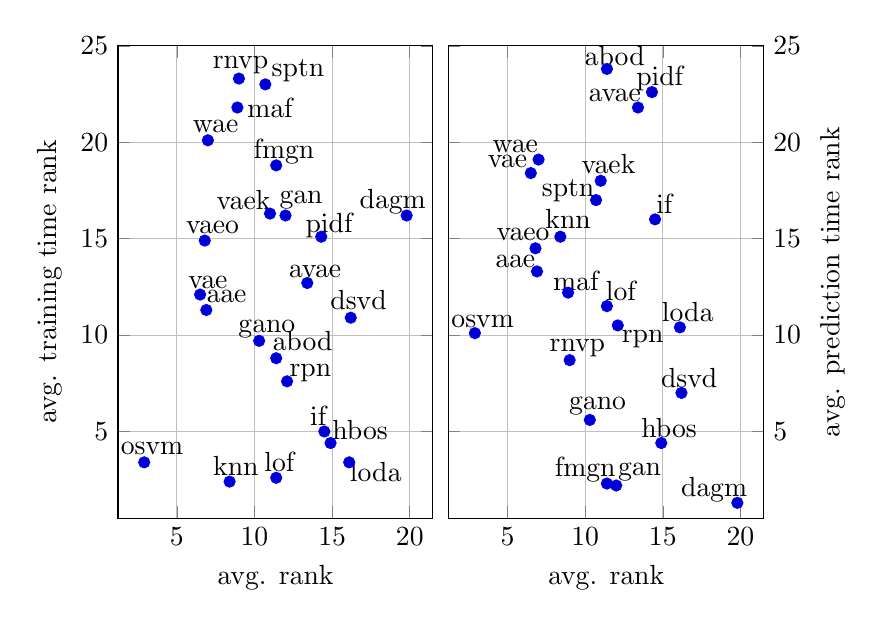
\begin{tikzpicture}[]
\begin{groupplot}[group style={vertical sep = 0.0cm, horizontal sep = 0.2cm, group size=2 by 1}]

\nextgroupplot [
  xlabel = {avg. rank},
  ylabel = {avg. training time rank},
  ylabel near ticks, yticklabel pos=left,
  ymin = 0.5, ymax=25,
  width=4cm, height=6cm, scale only axis=true,
  grid=major,
  % title = {(fit time)}
]

\addplot+[
  draw = none
] coordinates {
  (6.9, 11.3)
  (11.4, 8.8)
  (13.4, 12.7)
  (19.8, 16.2)
  (16.2, 10.9)
  (11.4, 18.8)
  (12.0, 16.2)
  (10.3, 9.7)
  (14.9, 4.4)
  (14.5, 5.0)
  (8.4, 2.4)
  (16.1, 3.4)
  (11.4, 2.6)
  (8.9, 21.8)
  % (22.3, 19.4)
  (2.9, 3.4)
  (14.3, 15.1)
  (9.0, 23.3)
  (12.1, 7.6)
  (10.7, 23.0)
  (6.5, 12.1)
  (11.0, 16.3)
  (6.8, 14.9)
  (7.0, 20.1)
};

\node at (axis cs:8.2, 12.0) {aae};

\node at (axis cs:13.1, 9.7) {abod};

\node at (axis cs:13.9, 13.3) {avae};

\node at (axis cs:18.9, 16.9) {dagm};

\node at (axis cs:16.7, 11.8) {dsvd};

\node at (axis cs:11.9, 19.5) {fmgn};

\node at (axis cs:13.0, 17.0) {gan};

\node at (axis cs:10.8, 10.3) {gano};

\node at (axis cs:16.8, 5.1) {hbos};

\node at (axis cs:14.1, 5.8) {if};

\node at (axis cs:8.8, 3.2) {knn};

\node at (axis cs:17.8, 2.9) {loda};

\node at (axis cs:11.6, 3.4) {lof};

\node at (axis cs:11.0, 21.8) {maf};

% \node at (axis cs:22.8, 20.0) {mgal};

\node at (axis cs:3.4, 4.1) {osvm};

\node at (axis cs:14.8, 15.7) {pidf};

\node at (axis cs:9.1, 24.0) {rnvp};

\node at (axis cs:13.6, 8.0) {rpn};

\node at (axis cs:12.8, 23.7) {sptn};

\node at (axis cs:7.0, 12.7) {vae};

\node at (axis cs:9.3, 17.0) {vaek};

\node at (axis cs:7.3, 15.6) {vaeo};

\node at (axis cs:7.5, 20.8) {wae};

\nextgroupplot [
  xlabel = {avg. rank},
  ylabel = {avg. prediction time rank},
  ylabel near ticks, yticklabel pos=right,
  ymin = 0.5, ymax=25,
  width=4cm, height=6cm, scale only axis=true,
  % title = {(evaluation time)},
  grid=major,
  % yticklabels={}
]

\addplot+[
  draw = none
] coordinates {
  (6.9, 13.3)    
  (11.4, 23.8)    
  (13.4, 21.8)
  (19.8, 1.3)
  (16.2, 7.0)
  (11.4, 2.3)
  (12.0, 2.2)
  (10.3, 5.6)
  (14.9, 4.4)
  (14.5, 16.0)
  (8.4, 15.1)
  (16.1, 10.4)
  (11.4, 11.5)
  (8.9, 12.2)
  % (22.3, 10.0)
  (2.9, 10.1)
  (14.3, 22.6)
  (9.0, 8.7)
  (12.1, 10.5)
  (10.7, 17.0)
  (6.5, 18.4)
  (11.0, 18.0)
  (6.8, 14.5)
  (7.0, 19.1)
};

\node at (axis cs:5.5, 13.8) {aae};

\node at (axis cs:11.9, 24.5) {abod};

\node at (axis cs:11.9, 22.4) {avae};

\node at (axis cs:18.3, 2.0) {dagm};

\node at (axis cs:16.7, 7.8) {dsvd};

\node at (axis cs:10.0, 3.0) {fmgn};

\node at (axis cs:13.5, 2.9) {gan};

\node at (axis cs:10.8, 6.3) {gano};

\node at (axis cs:15.4, 5.2) {hbos};

\node at (axis cs:15.1, 16.8) {if};

\node at (axis cs:8.9, 16.0) {knn};

\node at (axis cs:16.6, 11.2) {loda};

\node at (axis cs:12.3, 12.3) {lof};

\node at (axis cs:9.4, 12.8) {maf};

% \node at (axis cs:22.8, 10.7) {mgal};

\node at (axis cs:3.4, 10.7) {osvm};

\node at (axis cs:14.8, 23.3) {pidf};

\node at (axis cs:9.5, 9.3) {rnvp};

\node at (axis cs:13.7, 9.8) {rpn};

\node at (axis cs:8.9, 17.5) {sptn};

\node at (axis cs:5.0, 19.0) {vae};

\node at (axis cs:11.5, 18.9) {vaek};

\node at (axis cs:6.0, 15.2) {vaeo};

\node at (axis cs:5.5, 19.8) {wae};

\end{groupplot}
\end{tikzpicture}


        }
        \caption{tabular datasets}
        \label{fig:tabular_total_eval_t_fit_t_combined}
    \end{subfigure}
    \begin{subfigure}{\columnwidth}
        \centering
        \small
        \resizebox {\linewidth}{!}{
            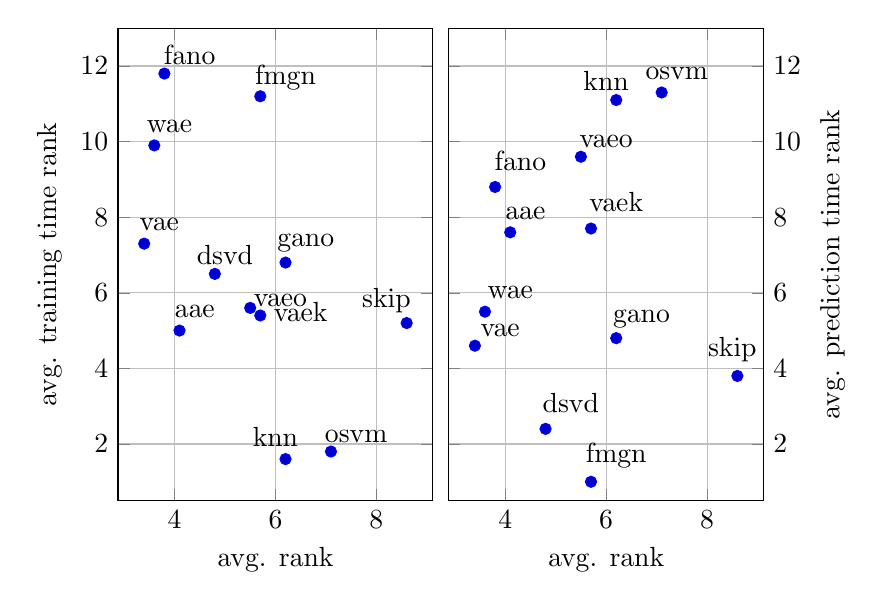
\begin{tikzpicture}[]
\begin{groupplot}[group style={vertical sep = 0.0cm, horizontal sep = 0.2cm, group size=2 by 1}]

\nextgroupplot [
  xlabel = {avg. rank},
  ylabel = {avg. training time rank},
  ylabel near ticks, yticklabel pos=left,
  ymin = 0.5, ymax=13,
  width=4cm, height=6cm, scale only axis=true,
  grid=major,
  % title = {(fit time)}
]

\addplot+[
  draw = none
] coordinates {
  (4.1, 5.0)
  (4.8, 6.5)
  (3.8, 11.8)
  (5.7, 11.2)
  (6.2, 6.8)
  (6.2, 1.6)
  (7.1, 1.8)
  (8.6, 5.2)
  (3.4, 7.3)
  (5.7, 5.4)
  (5.5, 5.6)
  (3.6, 9.9)
};

\node at (axis cs:4.4, 5.5) {aae};

\node at (axis cs:5.0, 7.0) {dsvd};

\node at (axis cs:4.3, 12.3) {fano};

\node at (axis cs:6.2, 11.7) {fmgn};

\node at (axis cs:6.6, 7.3) {gano};

\node at (axis cs:6.0, 2.2) {knn};

\node at (axis cs:7.6, 2.2) {osvm};

\node at (axis cs:8.2, 5.8) {skip};

\node at (axis cs:3.7, 7.8) {vae};

\node at (axis cs:6.5, 5.5) {vaek};

\node at (axis cs:6.1, 5.8) {vaeo};

\node at (axis cs:3.9, 10.4) {wae};

\nextgroupplot [
  xlabel = {avg. rank},
  ylabel = {avg. prediction time rank},
  ylabel near ticks, yticklabel pos=right,
  ymin = 0.5, ymax=13,
  width=4cm, height=6cm, scale only axis=true,
  % title = {(evaluation time)},
  grid=major,
  % yticklabels={}
]

\addplot+[
  draw = none
] coordinates {
  (4.1, 7.6)
  (4.8, 2.4)
  (3.8, 8.8)
  (5.7, 1.0)
  (6.2, 4.8)
  (6.2, 11.1)
  (7.1, 11.3)
  (8.6, 3.8)
  (3.4, 4.6)
  (5.7, 7.7)
  (5.5, 9.6)
  (3.6, 5.5)
};

\node at (axis cs:4.4, 8.1) {aae};

\node at (axis cs:5.3, 3.1) {dsvd};

\node at (axis cs:4.3, 9.5) {fano};

\node at (axis cs:6.2, 1.7) {fmgn};

\node at (axis cs:6.7, 5.3) {gano};

\node at (axis cs:6.0, 11.6) {knn};

\node at (axis cs:7.4, 11.8) {osvm};

\node at (axis cs:8.5, 4.5) {skip};

\node at (axis cs:3.9, 5.0) {vae};

\node at (axis cs:6.2, 8.4) {vaek};

\node at (axis cs:6.0, 10.0) {vaeo};

\node at (axis cs:4.1, 6.0) {wae};

\end{groupplot}
\end{tikzpicture}


        }
        \caption{image datasets}
        \label{fig:images_total_eval_t_fit_t_combined}
    \end{subfigure}
    \caption{Scatter-plots of the average rank in the AUC metric on the tabular  (a) and image (b) data versus average rank of the computational complexity of the displayed methods measured via training time (left) and prediction time (right). MO-GAAL has been omitted from the tabular figures, as its performance positioned it too far to the right with the training time rank of $19.4$ and the prediction time rank of $10.0$.}
    \label{fig:images_total_eval_t_fit_t_combined_joined}
\end{figure*}

Practitioners ask for fast and accurate algorithms, but these two features rarely go hand in hand, and a decision on a trade-off has to be made. Interesting methods lie on the Pareto frontier, as in the absence of an external factor, rationally behaving practitioner does not have a motivation to choose a different model.

Fig.~\ref{fig:tabular_total_eval_t_fit_t_combined}-left shows the trade-off between accuracy and training time for tabular data, where the absolute numbers were replaced by average ranks for robustness. The Pareto frontier contains two methods, which are OC-SVM and kNN. The position of OC-SVM is rather surprising, as its training time is known to scale poorly (quadratically) with respect to the number of samples, but it is caused by most of the tabular datasets being small. Different results may arise for a dataset with many data records. Fig.~\ref{fig:tabular_total_eval_t_fit_t_combined}-right shows a similar trade-off between accuracy and testing (inference) time. OC-SVM is still on the Pareto frontier, but it is expensive, as the complexity grows linearly in the number of samples. fmGAN, GAN and DAGMM methods are there as well -- these methods have fast inference but lower accuracy.

We provide results averaged over the studied contexts on image data. Due to the variability of the results in each context, the x-axis will vary. In the averaged ranks, VAE is on the Pareto front in both fit and prediction times, see Fig.~\ref{fig:images_total_eval_t_fit_t_combined}. Its prediction complexity is given mainly by choice of the number of samples taken in the computation of the sampled reconstruction score~\eqref{eq:score_sample}. The kNN detector has negligible training time, given only by the construction of the tree structure representing data, but seems to be mostly unusable on image data due to slow prediction times on datasets that are large in dimension and number of samples. The fmGAN finds itself in a completely reversed scenario.

\subsection{Other influences}
\label{sec:other_context}
In this section, we report the results of three sources of variability of performance of AD methods that were found to have minimal impact.

\emph{Ensembles/Hyperparameter averaging} The benefits of ensembles in prior art seem to be mixed. While~\cite{choiWAICWhyGenerative2019} claims that a combination of VAE or GAN ensembles using WAIC might be useful, Ref.~\cite{nalisnickDeepGenerativeModels2019} claims a negligible effect. In our experiments, we have used ensembles as a way to reduce uncertainty in hyperparameters~\cite{wilson2020case}, meaning that unlike in~\cite{choiWAICWhyGenerative2019}, models in ensembles were of a single type differing only in architecture. The effect of such an ensemble on average AUC was overall zero, sometimes even negative, see Supplementary~\ref{sec:appendix_ensembles}, Tab.~\ref{tab:ensembles_sensitivity_grouped}. Exceptions are methods based on GANs featuring improvements by $0.02$ in average AUC. These findings are on par with those in~\cite{nalisnickDeepGenerativeModels2019}.

\emph{Bayesian optimization} Bayesian optimization was introduced as an alternative to a random search of hyperparameters. It has the potential to find better hyperparameters with a low number of trials. Comparison of the random search and Bayesian optimization under the same conditions is reported in the Supplementary, Tab.~\ref{tab:tabular_bayes_comparison}. We can conclude that Bayesian optimization was able to find hyperparameters with better performance for the vast majority of the methods. However, this improvement is often quite small and insufficient to change the ranks of the methods. Notable exceptions are the GANomaly and GAN methods which improved by two ranks. 

\emph{Performance metric AUC/TPR} The hypothesis that the methods may perform differently when chosen for different optimization criteria than the usual AUC has not been proved. The results are summarized in the Supplementary, Tab.~\ref{tab:metric_comparison_grouped}. While small changes in performance have been observed, the ranks of the methods remain the same in both criteria, AUC and TPR@5\%. 

\section{Conclusion}
The presented extensive comparison of anomaly detection methods based on deep generative methods, namely variants of flows, variational autoencoders, and generative adversarial networks with methods based on alternative paradigms (Support vector machines, random forests, histogram, and distance-based methods) revealed that the performance of anomaly detection methods strongly depends on experimental conditions. We have identified the main sources of variation to be the choice of data and hyperparameter tuning. We presented detailed results under a combination of experimental conditions, called contexts, specifically the data context, hyperparameter context, and economic context. 

In the dataset context, a clear distinction in performance was found between tabular data, image data containing statistical and semantic anomalies. The main distinction in hyperparameter selection was how many anomalies were present in the validation set. Different order of performance of the tested method was observed for a different combination of dataset type and hyperparameter selection context, explaining various outcomes of comparison in the prior art. We strongly recommend that authors provide more details on the context of their experimental studies in the future.

The comparison is not only aimed at researchers but also at practitioners desiring accurate methods with low computational complexity. Therefore, we visualize these trade-offs between performance and computational cost. Also, we present a list of some of the most important practical observations and recommendations.
\begin{itemize}
    \item Methods with more exact likelihood modeling, such as kNN, flow, and autoencoder-based models, perform better in scenarios with a limited number of anomalies available for hyperparameter tuning.
    \item Majority of the methods fail to detect semantic anomalies. The exception is the fmGAN, but only if given enough computational resources and many anomalous samples for cross-validation. 
    \item OC-SVM, when properly tuned, can defeat most of the state-of-the-art on tabular data, although it suffers from overfitting when hyperparameters are selected using too few anomalies in the validation set.
    \item The method of the first choice appears to be the VAE/WAE due to its relatively cheap, precise, and consistent performance in most of the experiments. However, it possesses so many degrees of freedom that it forms a full family of methods. It was found that the best performance is obtained when estimating the full variance of samples on the output of the decoder and evaluating anomalies using sampled reconstruction score. 
\end{itemize}

Many aspects have not been covered and remain a topic of future work, such as the identification of the relevant kind of anomalies in the semantic datasets or the design of ensembles of methods of various types. Although we have shown that the number of anomalies available for validation is an important context, there was no further budget for a comparison of anomaly detection methods with active learning.  We have also completely left out the comparison of models on temporal data, such as time series or video, which is a very challenging task. Finally, an interesting area to study further is the influence of the presence of unlabeled anomalies in the training data.


\section{Anomaly detection with generative models: practical example} \label{sec:alfven}
In this section, an application of generative modelling on a practical example is presented. It was previously published in~\cite{vskvara2020detection}. Some of different generative autoencoders presented in Sec.~\ref{vae_models} will be used here to model data measured in a complex scientific experiment. Apart from the comparison of the previously presented anomaly scores, consider this to be a preliminary exploration of the already mentioned two-stage modeling principle, where an autoencoding model is used to create meaningful low-dimensional representation of complex data, and which is then coupled with some classical detector from Sec.~\ref{sec:taxonomy}. This concept will also be further explored in Chapter~\ref{sec:chapter_sgvaegan}.

\section{Chirping modes on the COMPASS tokamak}
\begin{figure}[t]%[!htbp]
  \centering
  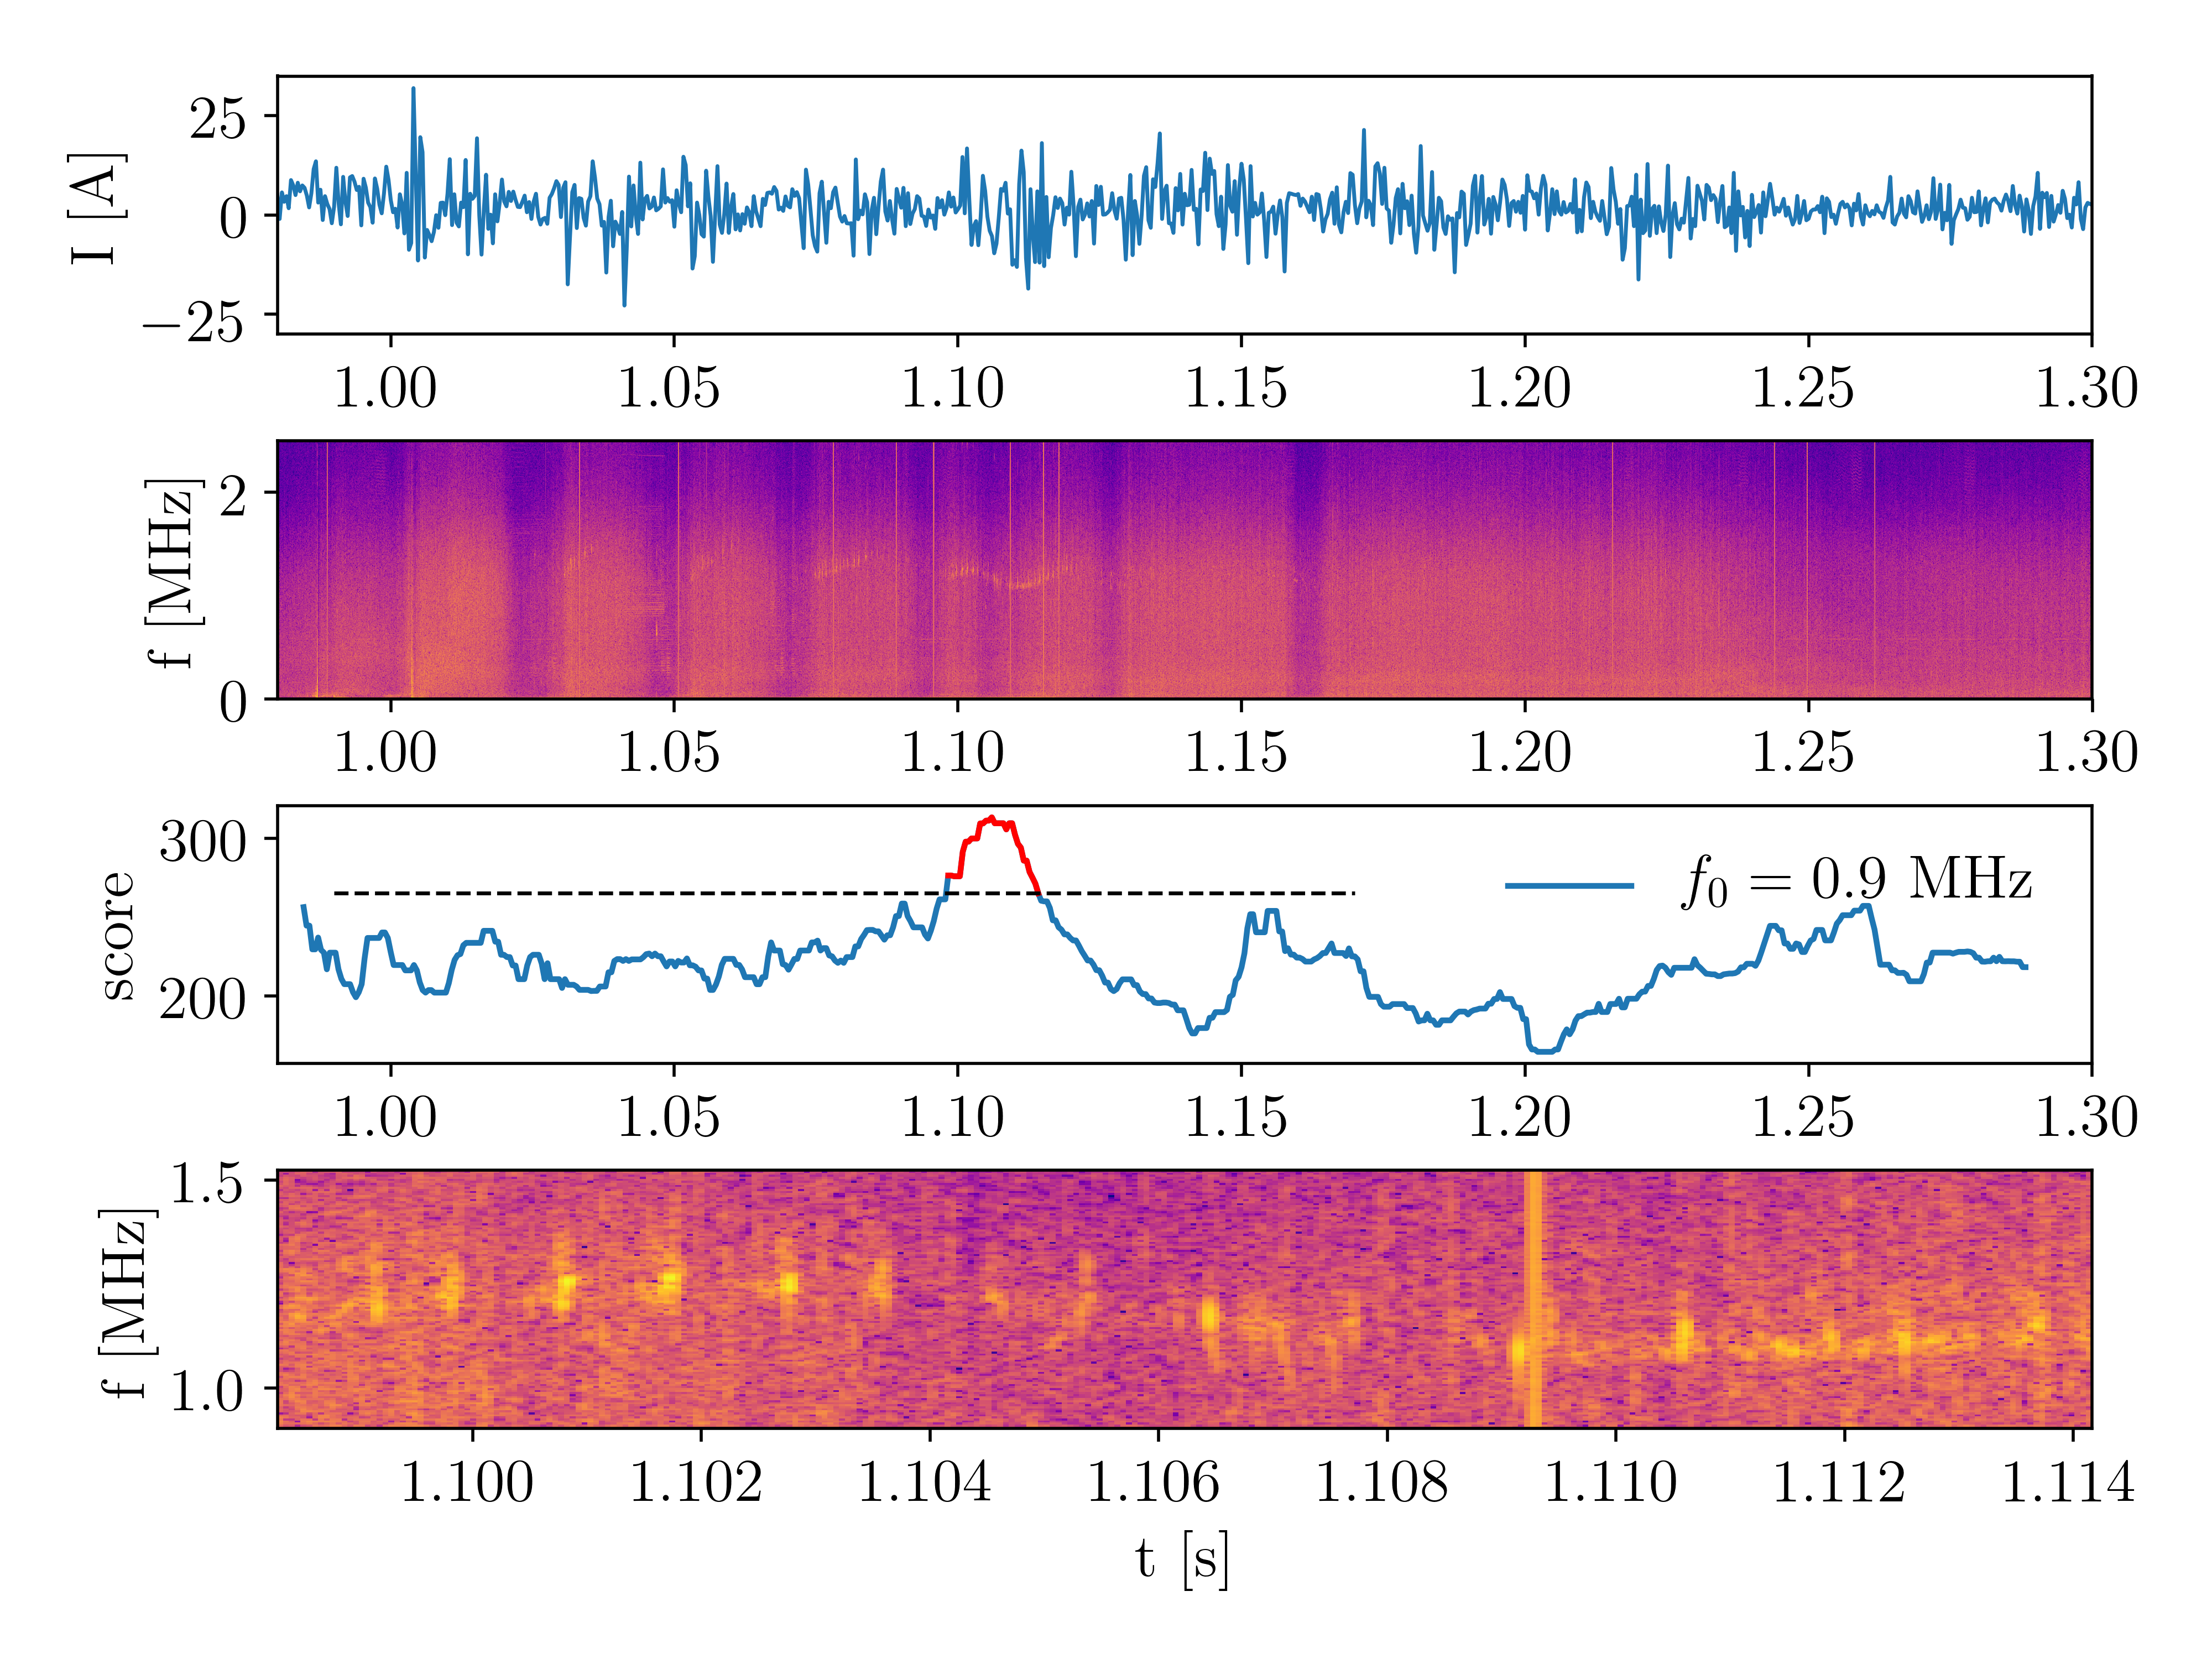
\includegraphics[scale=0.7]{data/chapter_alfven/overview.png}
  \caption{COMPASS shot 10870. Raw U-probe signal is in the upper plot. The corresponding spectrogram is below that. The score is the output of one of tested models over the spectrogram at $f_0=0.9$ MHz and it is plotted third from the top. The highest peak around 1.1s corresponds to a detected chirping mode. A close-up of the spectrogram part containing the chirping mode as detected from the red part of the score plot is at the bottom. The size of the close-up is 128 $\times$ 311 pixels.}
  \label{fig:psd}
\end{figure}

\subsection{The application problem}
As already mentioned in the introductory chapter, physics has recently enjoyed an influx of very large amounts of data~\cite{bird2011computing,ball2010data} that needs to be processed and most importantly, from which new scientific discoveries may be extracted. This is also true for the field of plasma fusion, which strives to ignite and control a fusion reaction as a clean and basically inexhaustible source of energy. The ITER project~\cite{holtkamp2007overview} is expected to produce up to 2 petabytes of data every day. This naturally calls for automatic processing of the data for a multitude of tasks, including anomaly detection. In this section, an anomaly detection problem that appears during the operation of the COMPASS~\cite{panek2015status} tokamak will be dissected.

During the operation of COMPASS, \textbf{Alfv\'en eigenmodes}~\cite{markovic2015alfven, melnikov2015quasicoherent, markovic2017alfven} were observed. Alfv\'en eigenmodes are magnetic instabilities that degrade the performance of the tokamak and possibly endanger and the plasma-facing components of the magnetic chamber~\cite{mett1992kinetic}. For this reason, their automatic detection is very important. Also, it may offer an opportunity for the study of their interactions with high-energy particles present in the plasma during an experiment. On COMPASS, chirping Alfv\'en eigenmodes are estimated to appear in about 0.1\% of all experiments. The primary means of their identification is manual inspection of spectrograms drawn from the signal of certain magnetic probes, which is very time-consuming. See Fig.~\ref{fig:psd} for an example of the measured signal, a spectrogram that is derived from it and a detected chirping Alfv\'en eigenmode. The spectrograms such as the one in Fig.~\ref{fig:psd} are large, so they are divided into patches of 128x128 pixels which is a feasible input size for current convolutional neural network architectures. It is also enough to capture most of a typical chirping mode as can be seen in the bottom plot in Fig.~\ref{fig:psd}. The patches that contain a chirping Alfv\'en eigenmodes are considered to be anomalies. There are about 200 labeled examples of patches with a chirping Alfv\'en eigenmode and a large database of unlabeled data. This is a typical anomaly detection problem, where labeled anomalies are only used for evaluation and comparison of different models and the training dataset is considered to be anomaly-free.

\subsection{The experimental setup}
Two basic experimental setups are tested in this section. Both are be based on generative autoencoders from Sec.~\ref{sec:vae_models}. The basic models have similar architectures, but they differ in the probability divergences used to regularize the latent space. The KLD~\eqref{eq:vae_kld} of a VAE model is compared against the MMD~\eqref{eq:mmd}. A WAE model with a discriminator is regularized by JSD which results in the training losses~\cite{eq:aae_loss_disc} and~\cite{eq:aae_loss_autoencoder}. Finally, a plain AE from Sec.~\ref{sec:reconstruction_models} is included to verify that a regularized latent space is useful. The individual components of the models (encoders, decoders, discriminators) are represented by neural networks with convolutional architecture. This is the most often used architecture for image data, as several levels of convolution operations are designed to capture shift invariant features at different scales of an image. For more technical details on the construction of the models, see~\cite{vskvara2020detection}. A schematic of a convolutional autoencoder is in Fig.~\ref{fig:ae}.

\begin{figure}[htpb]
\begin{center}
\begin{tikzpicture}[scale=1, transform shape]
  \vspace{-10cm}
  \node (image) at  (0,0) {\includegraphics[width=\linewidth]{data/chapter_alfven/model_structure.pdf}};
  \node (encdim) at (-4,\capy) {$\x \in \mathbb{R}^{128\times128\times1}$};
  \node (decdim) at (4,\capy) {$\hat{\x} \in \mathbb{R}^{128\times128\times1}$};
  \node (latdim) at (0, \capy) {$\z \in \mathbb{R}^{d}$};
  \node (enc) [align=left] at (\encx, .5) {encoder\\ $e_{\phi}(\x)$};%{$e_{\phi}(\x)$};
  \node (enc) [align=left] at (\encx, -.5) {Conv. +\\ Dense};
  \node (dec) [align=left] at (\decx, .5) {decoder\\ $d_{\theta}(\z)$};%{$d_{\theta}(\z)$};
  \node (dec) [align=left] at (\decx, -.5) {Dense +\\ Tr. Conv.};
\end{tikzpicture}
\end{center}
\caption{A schematic diagram of the convolutional autoencoder used for our experiments. Spectrogram patches are encoded through several convolutional\cite{lecun1989backpropagation}, maxpooling\cite{ranzato2007efficient} and dense (fully connected) layers into $d$-dimensional vectors (here $d=2$) and then decoded back with transposed convolutions and upscaling layers.}
\label{fig:ae}
\end{figure}

In the first setup, the described models are compared against each other as primary anomaly detectors. This means that they are trained on the (assumed) normal spectrogram patches and the anomaly scores derived in their respective sections are 


\subsection{One-class model}
In the first model, we will use a convolutional generative autoencoder as a one-class estimator. This is an approach well known in the anomaly/outlier detection setting\cite{chandola2009anomaly,scholkopf2001estimating}. A model of choice learns a representation of one class of data and can, therefore, be used to detect out-of-class samples. It is trained either with labeled data belonging to the class of interest, or with unlabeled data which are believed to contain so little out-of-class examples that the model is robust enough to ignore them. 

A generative autoencoder can be readily used for this task if we set $p_{\theta}(x) \approx p(x)$ to be the distribution of the class of our interest. Then there are two modes of training the autoencoder. In the first mode, we model the distribution of patches that contain a chirping mode. Then the autoencoder is trained with the positively labeled data. However, this is a bit problematic since there are very few labeled patches available, therefore the neural network will very likely overfit. In the second mode, we can choose the class of interest to be of the patches that do not contain a chirping mode. This is closer to an anomaly detection formulation of the problem, as the relatively rare chirping modes are considered to be anomalous. Also, the autoencoder can be trained with unlabeled data due to the sparse occurrence of chirping modes and robustness of probabilistic neural networks\cite{an2015variational,leveau2017adversarial}, hugely increasing the number of training samples and thus the representative power of the neural network. On the other hand, this might

To decide whether a sample $x$ is in- or out-of-class, we can compute its negative loglikelihood under the generative distribution 
\begin{equation} \label{eq:llh}
  -\mathbb{E}_{q_{\phi}(z|x)}\left[\ln p_{\theta}(x|z)\right]
\end{equation}
or its approximation, the MSE between $x$ and its (sampled) reconstruction $\hat{x}$. In our experiments, we use loglikelihood~\eqref{eq:llh} since it better captures the uncertainty in the reconstruction.

\subsection{Two-stage model}
The second model is designed to make the most use of both labeled and unlabeled data. It exploits the ability of generative autoencoders to produce low dimensional uncorrelated representation of high dimensional image data. It consists of two stages. The first stage is a convolutional generative autoencoder trained with unlabeled data. Its task is to learn the general topology of the input space and encode input data. The second stage is a classifier that is trained on encoded labeled data. Through the use of MMD or $\text{JS}_D$ measures and VampPrior, we can enforce separation of the encoded data into clusters that contain similar inputs, which makes the task of the classifier easier. Two different classifiers were tested.


\paragraph{kNN} The kNN algorithm for classification\cite{deng2016efficient} was trained using the labeled training data. In this setting, an unlabeled sample is given a score based on the average label of its $k$-nearest neighbors. The more neighboring training samples are labeled as positive, the higher the score.

\paragraph{GMM} A Gaussian Mixture Model (GMM)\cite{huang2005gaussian} with $M$ components was fitted on the latent representations of both labeled and unlabeled training data. Afterward, we determine one or more components of the mixture into which the positively labeled training samples are most likely to be projected via the encoder. Then, for a new sample, the score is the (average) loglikelihood of the sample in the anomalous components. 

\subsection{Experimental setup}

\subsection{Data}
Every spectrogram was divided into patches of size $128\times128$ pixels. Out of 40 pre-processed spectrograms, 370 non-overlaping patches were extracted and labeled. This results in a labeled training dataset $\left\{ X_{l},Y\right\} ,X_{l}=\left\{ x_{i}\right\} _{i},x_{i} \in \mathbb{R}^{128\times128\times1}, Y=\left\{ y_{i}\right\} ,y_{i}\in\left\{ 0,1\right\}$ of samples $X_{l}$ and labels $Y$, where $Y=1$ if a patch contains a chirping mode. Also, an unlabeled database $X_{u}$ of 330000 patches coming from 2000 spectrograms was created. 

Training of the one-class model was done both with labeled positive spectrograms and on the large unlabeled dataset. In the first case, the 50\% of positive spectrograms were used for training and the rest together with the unlabeled ones for testing. Also, training patches were randomly shifted and noise was added to them so that there were a total of $10^4$ training samples. In the second case, all of the labeled data was only used for testing. 10 different training and testing datasets were created this way for cross-validation purposes.

For training of the two-stage model, we have split the labeled dataset to training/testing subsets with the ratio 80/20. Again, this splitting was done randomly a total of 10 times.

\subsection{Model architecture and hyperparameters}

\begin{table}
\centering

\captionsetup[subtable]{position = below}
\captionsetup[table]{position=below}

\begin{subtable}{0.4\linewidth}
  \centering
  \begin{tabular}{c | c}
     parameter & values\tabularnewline
    \hline 
    $\gamma$ & $\left\{ 10^{0},10^{-1},10^{-2}\right\} $\tabularnewline
    $\lambda,\lambda_{1},\lambda_{2}$ & $\left\{ 10^{1},10^{0},10^{-1}\right\} $\tabularnewline
    $d$ & $\left\{ 8, 128,256\right\} $\tabularnewline
    
  \end{tabular}
  \caption{One-class model.}
  \label{tab:1c_params}
\end{subtable}
\hspace*{4em}
\begin{subtable}{0.4\linewidth}
  \centering
  \begin{tabular}{c  c | c}
      & parameter & values\tabularnewline
    \hline 
    \multirow{4}{*}{1st stage} & $N$ & $\left\{ 1,2,4,8\right\} $\tabularnewline
    & $\gamma$ & $\left\{ 10^{0},10^{-1},10^{-2}\right\} $\tabularnewline
    & $\lambda,\lambda_{1},\lambda_{2}$ & $\left\{ 10^{1},10^{0},10^{-1}\right\} $\tabularnewline
    & $d$ & $\left\{ 2,16,32,64\right\} $\tabularnewline
    \hline
    \multirow{2}{*}{2nd stage} & $k$ & $\left\{ 1,3,\ldots,31\right\} $\tabularnewline
    & $M$ & $\left\{ 2,4,6,8\right\} $\tabularnewline

  \end{tabular}
  \caption{Two-stage model.}
  \label{tab:2s_params}
\end{subtable}
\caption{Overview of model hyperparameters. $\lambda_{1}$ and $\lambda_{2}$ are scaling parameters for the combination of MMD and adversarial loss.}
\end{table}

\paragraph{One-class model}
The architecture for the one-class encoder was 2 or 3 convolutional layers with (32,64) or (32,32,64) channels and kernel size of 5. Each convolutional layer was followed by a maxpooling layer which downscaled the image by a factor of 2. Then a dense layer produced the final encoding into a $d$-dimensional latent space. The decoder mirrored the encoder architecture with transposed convolutions in place of maxpooling layers. ResNet\cite{he2016deep} type residual blocks were used to speed up and stabilize the training. The hyperparameter values over which we have optimized trained models are in Tab.~\ref{tab:1c_params}.
Parameter $\gamma$ denotes the scaling parameter of the inverse multiquadratics (IMQ) kernel\cite{gorham2017measuring}.

\paragraph{Two-stage model}
The basic encoder architecture was the following: 3 convolutional layers with (16,16,32) channels and kernel size of 3, (2,2,1) downscaling ratios via maxpooling, followed by two dense layers of width (256,$d$) where $d$ is the dimension of the latent space. The decoder mirrored this architecture. Also, batch normalization\cite{ioffe2015batch} was used. The hyperparameter values over which we have optimized are in Tab.~\ref{tab:2s_params}. The number of components in the used prior is denoted by $N$. 

The base architecture of the two models is slightly different. We have experimented with different architectures prior to the hyperparameter optimization and found that for the different tasks, different architectures provide better results. This is probably due to the fact that both models have a different objective - the one-class model requires precise reconstruction, while the two-stage is evaluated based on the shape of latent space. Ideally, we would include architectures as a tunable parameter, but that would require a level of computational power that was not available to us.

Both models use ReLu\cite{hahnloser2000digital} activation and were optimised with the RMSProp optimizer with learning rate $10^{-4}$. For a single optimization iteration, batches of 128 patches were used. We have implemented all the models in the Julia language\cite{bezanson2017julia} and trained them on TITAN V Nvidia GPU with 12 GB of memory. 

\section{Results}

In this section, the result of experiments with one-class and two-stage models are going to be examined and compared. Also, we will discuss the importance of an appropriate train/test splitting strategy that was used in our experiments in order not to obtain overly optimistic model performance estimates.

\subsection{Output evaluation}

\begin{figure}
\begin{centering}
\includegraphics[scale=0.5]{data/chapter_alfven/anomalies.png}
\par
\end{centering}
\caption{Examples of spectrogram patches identified as containing a chirping
mode.}
\label{fig:alfven_patches}
\end{figure}

In case our framework was implemented in a production environment, the working scenario would be the following. A set of experiments to be analyzed would be selected. Then, the needed signals would be extracted, spectrograms computed and divided into patches of appropriate size. These would be fed to a trained model that would produce scores to enable ranking of the patches. Since this would produce hundreds, maybe thousands of patches and scores, the operator would ideally only want to go through a few with the highest score. In Fig.~\ref{fig:alfven_patches} we show the output of such procedure --- 4 patches with the highest score, out of which 3 contain a chirping mode. It illustrates that even though the neural network encoding might be powerful, it is still basically a black box model and we need to be very careful in its evaluation. Because of this, we evaluate the model performance by computing AUC (area under the receiver operating curve), which is a standard measure for binary classification problems, and also by precision@$k$ score, which is the precision at the $k$-highest scoring samples. 

\subsection{One-class model optimization}

\begin{table}
  \centering
  \begin{tabular}[h]{c c c c} 
divergence & target class & AUC & precision@50 \\ 
\hline 
-- & Alfv\'en & $0.57 \pm 0.04$ & 0.24 $\pm$ 0.05 \\ 
KLD & Alfv\'en & 0.74 $\pm$ 0.06 & 0.44 $\pm$ 0.13 \\ 
MMD & Alfv\'en & 0.77 $\pm$ 0.03 & 0.49 $\pm$ 0.06 \\ 
JSD & Alfv\'en & 0.69 $\pm$ 0.07 & 0.42 $\pm$ 0.08 \\ 
MMD + JSD & Alfv\'en & 0.72 $\pm$ 0.09 & 0.37 $\pm$ 0.03 \\
-- & non--Alfv\'en & 0.82 $\pm$ 0.03 & 0.86 $\pm$ 0.06 \\ 
KLD & non--Alfv\'en & 0.46 $\pm$ 0.05 & 0.50 $\pm$ 0.14 \\ 
MMD & non--Alfv\'en & 0.84 $\pm$ 0.03 & \textbf{0.90 $\pm$ 0.06} \\ 
JSD & non--Alfv\'en & 0.84 $\pm$ 0.05 & 0.83 $\pm$ 0.10 \\ 
MMD + JSD & non--Alfv\'en & \textbf{0.84 $\pm$ 0.01} & 0.87 $\pm$ 0.01 \\ 
\end{tabular}

  \caption{Results of optimization of the one-class model. Target class differences are described in the experimental setup section. No divergence is a plain autoencoder with MSE training objective.}
  \label{tab:one_class}
\end{table}

The hyperparameter optimization routine resulted in hundreds of trained models. To select the best one, the AUC and precision@50 measures were computed on a testing dataset. Then, for a set of fixed hyperparameter values, these were averaged over 10 cross-validation test-train splits. The best results for a combination of target class and used divergence based on these measures are reported in Tab.~\ref{tab:one_class}. Clearly, it seems that modeling the distribution of chirping mode spectrograms is more difficult than vice versa with the exception of KLD, which completely fails. Also, the precision in top samples is very low in the Alfv\'en target class. Surprisingly, a plain autoencoder achieves results almost comparable to other models. In Fig.~\ref{fig:roc_prc} are the ROC (receiver operating characteristic)\cite{fawcett2006introduction} and PR (precision-recall)\cite{boyd2013area} curves of the single best performing one-class models as well as the two-stage models.

\begin{figure}
\begin{centering}
\includegraphics[scale=0.6]{data/chapter_alfven/roc_prc.pdf}
\end{centering}
\caption{ROC and PR curves of selected models.}
\label{fig:roc_prc}
\end{figure}

\subsection{Two-stage model}

\begin{table}
\centering
\begin{tabular}{c c c c}
	\toprule
	divergence & classifier & AUC & precision@50  \\
	\midrule
	-- & kNN & 0.80$\pm$0.07 &  \cellcolor{gray!15} 0.88$\pm$0.10 \\
	KLD & kNN & 0.80$\pm$0.08 & 0.85$\pm$0.11 \\
	MMD & kNN &  \cellcolor{gray!45} 0.91$\pm$0.06 &  \cellcolor{gray!45} 0.94$\pm$0.05\\
    JSD & kNN &  \cellcolor{gray!15} 0.83$\pm$0.07 & 0.87$\pm$0.10\\
    MMD + JSD & kNN &  \cellcolor{gray!30} 0.86 $\pm$ 0.07 &  \cellcolor{gray!30} 0.91$\pm$0.10 \\
    -- & GMM & 0.75$\pm$0.06 & 0.80$\pm$0.10\\
	KLD & GMM & 0.74$\pm$0.06 & 0.83$\pm$0.11\\
	MMD & GMM & 0.66$\pm$0.12 & 0.72$\pm$0.12\\
    JSD & GMM & 0.74$\pm$0.06 & 0.82$\pm$0.11\\
    MMD + JSD & GMM & 0.76$\pm$0.06 & 0.84$\pm$0.10 \\
    \bottomrule
\end{tabular}
\caption{Results of hyperparameter tuning of the two-stage model across 10 cross-validation splits.}
\label{tab:alfven_results}
\end{table}

Here, we evaluate the performance of the two-stage model. The methodology of hyperparameter optimization via cross-validation is similar to that used for the one-class model.  The best average result across 10 splits for different combinations of stage one divergences and stage two classifiers are reported in Tab.~\ref{tab:alfven_results}. The simple kNN model is superior to the GMM approach. Also, MMD regularization seems to produce the best results. We might speculate that this might be due to the improved ability to produce a well-separated encoding enforced by the used prior. Again, in Fig.~\ref{fig:roc_prc} see the ROC and PRC curves for the single best two-stage models.

A question one might ask is whether the autoencoding is truly necessary. In the end, we are doing a projection from $d=128\times128=16384$ dimensional picture space into at most $d=64$ dimensional latent space which must naturally lead to a loss of information. As shown in Fig.~\ref{fig:patches_latent}, where $d=8$, the autoencoder is able to identify the difficult nonlinear correlations and improve the performance of a subsequent second stage kNN model. The compression is clearly necessary for overcoming the curse of dimensionality which implies that L$_2$ distance degenerates in large dimensions. An alternative approach to overcoming the issue of large input dimension might be to train a classification convolutional neural network, which does the compression by its nature. We have not chosen to go this path however since we believe that such a network would be highly susceptible to overfitting since it requires a lo of labeled data which is not available to us. Instead, we have tried to overcome this in the two-stage model by learning the compression from all the available unlabeled data.

\subsection{Influence of the train/test splitting methodology}

\begin{figure}
\centering
\includegraphics[scale=0.45]{data/chapter_alfven/split_patches.pdf}
\includegraphics[scale=0.45]{data/chapter_alfven/split_spectrograms.pdf}
\caption{kNN fits for different values of $k$. The red line and band show the mean and one standard deviation bands of the resulting AUC values when kNN is fitted to the original vectorized images. The input space dimensionality is $d=16384$. The blue dashed line and band are the same quantities for a $d=8$ dimensional representation by a first stage model. On the left, the training and testing splits were done on the level of individual patches, leading to a better performance and less variance. On the right, the split was done on the level of the original spectrograms, which is a more realistic scenario. The standard deviation and mean were computed from 10 random splits.}
\label{fig:patches_latent}
\end{figure}

At first, the splitting of testing and training labeled patches was done on the level of patches, without any regard for the spectrogram/experiment that the patch came from. It was assumed that the labeled chirping modes are homogeneous across the spectrograms. However, this turned out not to be true. Therefore, the train/test splits were done on the level of spectrograms which were then subsequently divided into patches. See Fig.~\ref{fig:patches_latent} where on the left side, the AUC curves for different values of $k$ of the kNN model are for the case when the data split was done on the level of patches. The blue line that is the result of kNN fit peaks at $k=3$. On the other hand, there is no such peak on the right side of the figure, where splitting was done on the level of spectrograms. This indicates that the positively labeled patches in a single spectrogram are much more similar to each other than to those in different spectrograms, as only a relatively low number of neighbors is sufficient for optimal performance. Also, the variance of the right side plots is much higher, again indicating larger differences across spectrograms. If we continued with the splitting on the level of patches, we would have a biased and too optimistic estimate of performance before putting the framework into production.

\section{Conclusion}
Our task was identification of anomalous phenomena --- chirping Alfv\'en modes --- in graphical representations of signals measured during the operation of a tokamak. To this end, we have proposed two models based on generative autoencoders. The first model learned the distribution of normal data and identified chirping modes as out-of-class samples of this distribution. The second model implemented a two-stage learning approach. A regularized convolutional variational autoencoder trained on unlabeled data was successfully combined with a classifier trained with a smaller labeled dataset. It has been shown that both models are viable options in chirping mode identification, although the latter one proved to be superior.

We have also shown the need for proper cross-validation splitting of data in the evaluation phase and outlined the need for careful evaluation in order for the model to be useful in real-world application. However, this is still work in progress. We mentioned the need to use a more appropriate evaluation measure that reflects the operational conditions. Furthermore, so far we have only used spectrograms from a single U probe, but there are about 40 more magnetic diagnostics that could be potentially used for this task, e.g. their spectrograms/correlograms could be added as an additional input channel. Finally, a more thorough evaluation of the contemporary experimental results is needed for the understanding of the framework behavior and to be applicable to COMPASS operation, most likely through the expansion of the labeled dataset. 


\chapter{Anomaly detection in multi-factor data}

% write that we have shown that we need some kind of mechanism that is able to learn the individual parts of an image in order to detect semantic anomalies
% we have tried different models of unsupervised disentanglement
% it was shown somewhere theoretically that it is actually impossible
% all succesful disentanglement techniques use some kind of label information
% we will simply expect the image to contain a distinct background and foreground

\section{Motivation}

\section{Proposed method}

\subsection{SGVAE model}

\subsection{SGVAEGAN model}

\section{Experiments}

\subsection{Data and additional setup}

\subsection{Examples of how the model works}

\subsection{Classical comparison}

\subsection{Identification of anomaly types}



\chapter{Conclusion} \label{sec:conclusion}
In this chapter, we summarize the individual chapters of the dissertation and their relationship to original contributions that were published as peer-reviewed papers or are publicly available in the form of preprints. Also, we try to evaluate the goals that were set in the introduction in Sec.~\ref{sec:objectives}. Finally, we offer an outlook on future work.

\section{Contributions}
\paragraph{Chapter~\ref{sec:chapter_intro}} This chapter sets the playing field for the rest of the text with definitions of basic terms and ideas that are important for anomaly detection. It also introduces basic types of anomalies and sets a list of objectives that we are going to evaluate.

\paragraph{Chapter~\ref{sec:chapter_shallow}} This chapter contains an introduction to measures available for comparison of anomaly detectors, which is an excerpt from the paper~\cite{vskvara2023auc}, where the goal was to determine whether the standard AUC is the most suitable measure for anomaly detector comparison, as it has some weaknesses. Besides the theoretical description present here, the paper also contains an extensive experimental comparison. Besides that, Chapter~\ref{sec:chapter_shallow} also contains an extensive description of the current state-of-the-art shallow anomaly detectors, which partly covers the first objective from Sec.~\ref{sec:objectives}.

\paragraph{Chapter~\ref{sec:chapter_survey}} The rest of the first objective is covered in this chapter with an extensive description of deep anomaly detectors. Special attention is given to detectors based on deep generative models. We believe it is useful both for novices and experienced researchers in the field of generative models and/or anomaly detection as we strived to distill our knowledge of this topic in a digestible yet comprehensive manner.

In Sec.~\ref{sec:alfven}, the practical use of generative autoencoders is presented in the context of anomaly detection problems in plasma fusion physics. It was published as a journal paper~\cite{vskvara2020detection}. It provides inspiration for the following chapters because it shows the feasibility of a two-stage approach, where a deep model is coupled with a shallow one operating on the latter model's low-dimensional representations of otherwise high-dimensional inputs.

\paragraph{Chapter~\ref{sec:chapter_comparison}} Here, the main results of the paper~\cite{vskvara2021comparison}, which is a large-scale theoretical and experimental survey of deep generative models in anomaly detection, are presented. Its goals were to find a research direction in which generative anomaly detectors gain an advantage over other approaches, and it was successful in doing so, as it inspired the model proposed in Chapter~\ref{sec:chapter_sgvaegan}. Also, this paper itself is a continuation of the original publication~\cite{vskvara2018generative}, which had the same goals, but a much lesser scope.

This chapter fully covers the second objective that was set in Sec.~\ref{sec:objectives} by providing insights into: i) the effect of building blocks of anomaly detection on their performance, and ii) the generally poor performance of the existing methods on semantic image anomalies, which is the focus of the following chapter.

\paragraph{Chapter~\ref{sec:chapter_sgvaegan}} This is the product of the previous chapters and the main contribution of the thesis, which also covers the last objective set in Sec.~\ref{sec:objectives}. In this chapter, we present a novel multi-factor anomaly detection scheme. The scheme is demonstrated on a novel SGVAEGAN model which performs successfully on the problem of semantic anomaly detection on image data. It also provides a novel manner of informed but unsupervised image disentanglement and most importantly a procedure for anomaly origin detection and explanation, which is something that is missing in the current state-of-art of image anomaly detection. At the time of the writing of this thesis, it is currently considered for publication.

Finally, one of the contributions of this work is that it contains links to all the related software developed during our research process. The list of publicly available repositories is in Appendix~\ref{sec:appendix_links}.

\section{Future work}
As the field of anomaly detection progresses, novel methods appear constantly. In the vein of Chapter~\ref{sec:chapter_comparison}, we should strive to add novel methods into a fair comparison that evaluates them from different perspectives. Although this is clearly not feasible to do continuously, an updated version of such a survey, created after a few years, would be helpful in assessing how the field of anomaly detection has evolved in the meantime. In fact, when publishing the original article~\cite{vskvara2021comparison}, we knew that there were novel methods that appeared during the publication process and which we would have liked to cover as well. Furthermore, the conclusion of Chapter~\ref{sec:chapter_comparison} covers some missing topics, such as anomaly detection with active learning or temporal anomaly detection, which is a research area that has been gaining a lot of momentum recently.

Possible technical improvements of the model proposed in Chapter~\ref{sec:chapter_sgvaegan}, such as the use of a more flexible latent prior, are mentioned at the end of that chapter. Although the SGVAEGAN model was specifically designed for anomaly detection on images where a prominent object is positioned on a distinct background, the general approach to anomaly detection via disentanglement based on Eq.~\eqref{eq:alphadeco} is possibly applicable to a different kind of data where there there is a possibility of anomalies coming from different independent sources. Finally, we believe that in order to improve the understanding of the proposed model behaviour, its capabilities would be best demonstrated in new experiments on some real--world application data.

% ------------------------------------------------------------------------------
% Appendix
% ------------------------------------------------------------------------------
\part*{Apendices}

% what is in the appendices will be decided later
\input{chapters/appendix_01.tex}

% ------------------------------------------------------------------------------
% Bibliography
% ------------------------------------------------------------------------------
\cleardoublepage
\phantomsection

\addcontentsline{toc}{chapter}{Bibliography}
\bibliography{references.bib}
\bibliographystyle{unsrt}

\end{document}